% AMUN Wind Paper, based on:
% mnras_template.tex
%
% LaTeX template for creating an MNRAS paper
%
% v3.0 released 14 May 2015
% (version numbers match those of mnras.cls)
%
% Copyright (C) Royal Astronomical Society 2015
% Authors:
% Keith T. Smith (Royal Astronomical Society)

% Change log
%
% v3.0 May 2015
%    Renamed to match the new package name
%    Version number matches mnras.cls
%    A few minor tweaks to wording
% v1.0 September 2013
%    Beta testing only - never publicly released
%    First version: a simple (ish) template for creating an MNRAS paper

%%%%%%%%%%%%%%%%%%%%%%%%%%%%%%%%%%%%%%%%%%%%%%%%%%
% Basic setup. Most papers should leave these options alone.
\documentclass[a4paper,fleqn,usenatbib]{mnras}

% MNRAS is set in Times font. If you don't have this installed (most LaTeX
% installations will be fine) or prefer the old Computer Modern fonts, comment
% out the following line
\usepackage{newtxtext,newtxmath}
\usepackage{makecell}
% Depending on your LaTeX fonts installation, you might get better results with one of these:
%\usepackage{mathptmx}
%\usepackage{txfonts}

% Use vector fonts, so it zooms properly in on-screen viewing software
% Don't change these lines unless you know what you are doing
\usepackage[T1]{fontenc}
\usepackage{ae,aecompl}


%%%%% AUTHORS - PLACE YOUR OWN PACKAGES HERE %%%%%

% Only include extra packages if you really need them. Common packages are:
\usepackage{graphicx}	% Including figure files
\usepackage{amsmath}	% Advanced maths commands
\usepackage{amssymb}	% Extra maths symbols
\usepackage{amsfonts}
\usepackage{hyperref}
\usepackage{pifont}

%%%%%%%%%%%%%%%%%%%%%%%%%%%%%%%%%%%%%%%%%%%%%%%%%%

%%%%% AUTHORS - PLACE YOUR OWN COMMANDS HERE %%%%%

% Please keep new commands to a minimum, and use \newcommand not \def to avoid
% overwriting existing commands. Example:
%\newcommand{\pcm}{\,cm$^{-2}$}	% per cm-squared
\usepackage{abbrevs}
\usepackage{xspace}

% FORCE ROMAN FONTS IN SUBSCRIPTS
\begingroup
\catcode`\_=\active
\gdef_#1{\ensuremath{\sb{\mathrm{#1}}}}
\endgroup
\mathcode`\_=\string"8000
\catcode`\_=12


% Revision
% \newcommand{\rev}{\textcolor{Plum}}
\newcommand{\rev}{\textcolor{Black}}

% Useful abbreviations
\newcommand{\Msolar}{M$_{\odot}$\xspace}
\newcommand{\Msolarpc}{M$_{\odot}$ / pc$^{2}$\xspace}
\newcommand{\Zsolar}{Z$_{\odot\xspace}$\xspace}
\newcommand{\Rsolar}{R$_{\odot\xspace}$\xspace}
\newcommand{\Subvir}{$_{vir}$\xspace}
%\newcommand{\atcc}{atoms/cm$^{3}$\xspace}
\newcommand{\atcc}{cm$^{-3}$\xspace}
\newcommand{\mhcc}{m$_{H}$.cm$^{-3}$\xspace}
\newcommand{\simname}{\textsc}
\newcommand{\Stromgren}{Str\"{o}mgren\xspace}
\newcommand{\starsub}{$_{\normalfont\textsc{stars}}$\xspace}
\newcommand{\stars}{\textsc{stars}\xspace}
\newcommand{\turbsub}{$_{\normalfont\textsc{turb}}$\xspace}
\newcommand{\turb}{\textsc{turb}\xspace}
\newcommand{\rcoeff}{$\rho_{X,SFE}$}
\newcommand{\AMUN}{\textsc{amun}}
\newcommand{\HII}{H$~$\textsc{ii}\xspace}

% Graphical commands
%\newcommand{\tick}{$\checkmark$}
\newcommand{\tick}{\hspace{1pt}\ding{51}}
\newcommand{\cross}{\hspace{1pt}\ding{55}}

% Abbreviations
\newabbrev\ISM{Interstellar Medium (ISM)}[ISM]
\newabbrev\IGM{Intergalactic Medium (IGM)}[IGM]
\newabbrev\CSM{Circumstellar Medium (CSM)}[CSM]
\newabbrev\WNM{Warm Neutral Medium (WNM)}[WNM]
\newabbrev\WIM{Warm Ionised Medium (WIM)}[WIM]
\newabbrev\CNM{Cold Neutral Medium (CNM)}[CNM]
\newabbrev\IMF{Initial Mass Function (IMF)}[IMF]
\newabbrev\CMF{Core Mass Function (IMF)}[IMF]
\newabbrev\AMR{Adaptive Mesh Refinement (AMR)}[AMR]
\newabbrev\HGB{Horizontal Giant Branch (HGB)}[HGB]
\newabbrev\SFE{Star Formation Efficiency (SFE)}[SFE]
\newabbrev\TSFE{Total Star Formation Efficiency (TSFE)}[TSFE]
\newabbrev\OSFE{Observed Star Formation Efficiency (OSFE)}[OSFE]
\newabbrev\SFR{Star Formation Rate (SFR)}[SFR]
\newabbrev\YSOs{Young Stellar Objects (YSOs)}[YSOs]
\newabbrev\YSO{Young Stellar Object (YSO)}[YSO]
\newabbrev\PDF{Probability Distribution Function}[PDF]
\newabbrev\PSF{Point Spread Function}[PSF]
\newabbrev\LMC{Large Magellanic Cloud}[LMC]

% Table gunk
\renewcommand\theadalign{bc}
\renewcommand\theadfont{\bfseries}

\makeatletter
\newcommand*\bigcdot{\mathpalette\bigcdot@{.5}}
\newcommand*\bigcdot@[2]{\mathbin{\vcenter{\hbox{\scalebox{#2}{$\m@th#1\bullet$}}}}}
\makeatother

% Some gumf that makes spaces work properly because abbrevs is buggy: 
% See: http://tex.stackexchange.com/questions/59840/how-to-prevent-getting-a-space-after-an-abbreviation-using-the-abbrevs-package
\makeatletter
\renewcommand\maybe@space@{%
	% \@tempswatrue % <= this is in the original
	\maybe@ictrue % <= this is new
	\expandafter   \@tfor
	\expandafter \reserved@a
	\expandafter :%
	\expandafter =%
	\nospacelist
	\do \t@st@ic
	% \if@tempswa % <= this is in the original
	\ifmaybe@ic % <= this is new
	\space
	\fi
}
\makeatother
% Gumf ends

%%%%%%%%%%%%%%%%%%%%%%%%%%%%%%%%%%%%%%%%%%%%%%%%%%

%%%%%%%%%%%%%%%%%%% TITLE PAGE %%%%%%%%%%%%%%%%%%%

% Title of the paper, and the short title which is used in the headers.
% Keep the title short and informative.
\title[Are Winds Effective?]{Stellar Winds Don't Do Much Dynamically But They Also Volume Fill So It's Difficult To Say If They're Effective Or Not}

% The list of authors, and the short list which is used in the headers.
% If you need two or more lines of authors, add an extra line using \newauthor
\author[Geen et al]{
Sam Geen,$^{1}$\thanks{E-mail: s.t.geen@uva.nl}
Rebekka Bieri,$^{2}$
Joakim Rosdahl,$^{3}$
Alex de Koter$^{1}$
\\
% List of institutions
$^{1}$ Anton Pannekoek Institute for Astronomy, Universiteit van Amsterdam, Science Park 904, 1098 XH Amsterdam, The Netherlands\\
$^{2}$ Max-Planck-Institute for Astrophysics, Karl-Schwartzschild-Strasse 1, Garching, Germany\\
$^{3}$ CRAL, Universit\'e de Lyon 1, CNRS UMR 5574, ENS-Lyon, 9 Avenue Charles Andr \'e, 69561, Saint-Genis-Laval, France\\
}

% These dates will be filled out by the publisher
%\date{Accepted XXX. Received YYY; in original form ZZZ}
\date{\today}

% Enter the current year, for the copyright statements etc.
%\pubyear{2018}

% Don't change these lines
\begin{document}
\label{firstpage}
\pagerange{\pageref{firstpage}--\pageref{lastpage}}
\maketitle

% Abstract of the paper
\begin{abstract}
Stellar winds contribute a large amount of energy (``feedback'') to their surroundings by driving hot cavities into molecular clouds. In this paper, we use radiative magnetohydrodynamic simulations of molecular clouds containing individual stars of 30, 60 and 120 solar masses to study the relative effectiveness of winds and ionising radiation, and address the still open question of whether or not winds are effective at driving outflows. We find that winds contribute to bulk properties such as star formation efficiency and radial momentum carried by the feedback structures around the star at 10\% of the level of photoionisation feedback. Most of the energy from winds is lost to radiative cooling in the interface between the hot wind bubble and the photoionised gas, while the radiative cooling rate from the wind bubble is a few percent of the wind luminosity ($\frac{1}{2} \dot{m} v^2$). The complex ``chimney-and-plume'' geometry of the wind bubble suggests that the bubble is volume-filling, despite not being the principal driver of the outflows. However, additional effects such as radiation pressure may boost the relative effectiveness of winds. We find that winds from individual stars are not significant drivers of feedback, but they nonetheless shape their environment in complex ways.
\end{abstract}

% Select between one and six entries from the list of approved keywords.
% Don't make up new ones.
\begin{keywords}
stars: massive, 
stars: formation $<$ Stars, 
ISM: H ii regions, 
stars: winds, outflows,
ISM: clouds $<$ Interstellar Medium (ISM), Nebulae,
methods: numerical $<$ Astronomical instrumentation, methods, and techniques
\end{keywords}

%%%%%%%%%%%%%%%%%%%%%%%%%%%%%%%%%%%%%%%%%%%%%%%%%%

%%%%%%%%%%%%%%%%% BODY OF PAPER %%%%%%%%%%%%%%%%%%

\section{Introduction}
\label{introduction}

CITE https://arxiv.org/pdf/1910.06976.pdf AND PREVIOUS PAPER

ZSOLT COMMENT: WORK ON NARRATIVE OF MIDDLE OF INTRODUCTION

Stars form from dense clouds of gas that accrete onto the star. Energy emitted by stars is sometimes termed ``feedback'', because in sufficient quantities it has the capability to regulate future star formation. This is a multi-scale process, since it occurs on many scales. On the smallest scales, stars regulate their own formation. This has been simulated by \cite{Kuiper2018} for massive stars, and by \cite{Bate2019} for clusters of less massive stars, amongst others. Stars also regulate gas flows on cloud scales of 1-100 pc \citep[see review by][]{Dale2015a}, create hot and warm regions and drive turbulence in the interstellar medium of galaxies \cite[e.g.][]{Gatto2017} and even drive flows out of galaxies \citep[see review on galactic winds by][]{Veilleux2005} and shape the ionisation state of most of the volume of the universe \citep[e.g.][]{Rosdahl2018}.

In this paper we focus on the interaction between two feedback processes on cloud scales, namely photoionisation and winds, in the first Myr of the star's main sequence. Photoionisation feedback is driven by the ionisation of interstellar material by photons above the ionisation energy of hydrogen (13.6 eV). This heats the gas to approximately $10^4$ K, which creates a pressure difference between the ionised gas and neutral material outside, causing a pressure wave that expands outwards. The second is stellar winds, i.e. the ejection of material from the surface of the star through radiation pressure in the star's envelope. In massive stars, this material can be accelerated to thousands of km/s. Both of these processes carry large amounts of energy in massive stars. Observational evidence of this is seen in surveys by, e.g., \cite{Doran2013}. However, it is not immediately obvious how these processes interact, and which process has the biggest impact on its surroundings.

Early analytic work by \cite{KahnF.D.1954}, \cite{SpitzerLyman1978}, \cite{Whitworth1979} and others confirms that photoionisation feedback is indeed capable of driving strong flows into the interstellar medium. The same is true in analytic work focussed on adiabatic stellar wind bubbles, or bubbles of hot gas driven by stellar winds, by \cite{Avedisova1972}, \cite{Castor1975} and \cite{Weaver1977}.

More recently, authors have studied the interaction between these two processes in more detail. Analytic calculations by \cite{Capriotti2001} suggest that winds are likely not to have a significant dynamical effect on the expansion of \HII regions compared to photoionisation. \cite{Krumholz2009} argue that leakage from stellar wind bubbles further reduces the dynamical input from winds, because pressure acting on the surface of the bubble is lost to the ambient medium. The analytic and hydrodynamic models of \cite{Haid2018} confirm this in a cloud environment, but argue that once the wind has entered the already ionised interstellar medium, photoionisation cannot drive further outflows and winds are required. 

The radiative cooling of wind bubbles reduces their efficiency by removing energy from the bubble. \cite{MacLow1988} invoke two modes of cooling, one in the bubble itself and one by evaporation and mixing from the dense shell into the bubble, the first of which is generally most effective. In a molecular cloud environment, this timescale is typically shorter than the lifetime of the star. 

\cite{Silich2013} and \cite{Silich2018} produce two models, one in which the wind is adiabatic, and another which radiates efficiently and is driven purely by the instantaneous momentum input from the wind. These models are adopted by \cite{Rahner2017}, whose models transition between these modes after the cooling time in \cite{MacLow1988}. For massive clusters, winds do contribute a significant fraction of the force acting on the \HII region, peaking at around 3 Myr when massive stars begin to emit stronger winds during the Wolf-Rayet phase. However, \cite{Silich2017} argue that this depends on the ability for the wind bubbles around individual stars to merge, with isolated wind bubbles being less effective. \cite{Fierlinger2016} argue that winds in their work deposit around 2-3 times the energy from supernovae into the surrounding material, and further that careful modelling of the mixing of hot and cold gas at the bubble interface is crucial for obtaining correct bubble cooling rates.

\cite{Harper-Clark2009}, \cite{Yeh2012} and \cite{Yeh2013} construct quasi-static 1D models of \HII regions including photoionisation, radiation pressure and winds. They argue that models in which winds are not dynamically significant are consistent with nearby observed \HII regions. However, \cite{Pellegrini2007}, \cite{Pellegrini2011} and \cite{Pellegrini2012} argue that winds are required to explain the observed structure of these regions. This is dynamically significant since it sets the density of the photoionised region. However, they argue that there are certain regions, such as the Orion Veil, for which pressure equilibrium has not been reached and which diverge from such quasi-static models. \cite{Guedel2007} find extended x-ray emission inside this structure, arguing that winds are efficient in this region. \cite{Pabst2019} argue that such regions are best explained by adiabatic wind models, since the shells travel faster than the sound speed in ionised gas and the cooling from x-ray emission is low. \cite{Kruijssen2019} also argue that the depletion of molecular clouds by adiabatic winds and photoionisation should occur on similar timescales. 

Because these analyses do not always agree, there is thus a need for more comprehensive, if costly, self-consistent hydrodynamic simulations that include radiative transfer to study this phenomenon. In this paper we focus on molecular cloud scales. Simulations on protostellar \citep[e.g.][]{Kuiper2018} \ISM \citep[e.g][]{Gatto2017} and galactic \citep[e.g.][]{Agertz2013} scales have considered the role of stellar winds in feedback in those regimes. These works argue that on smaller scales, winds require protostellar jets and outflows to be efficiently launched, while at larger scales winds add to the thermal pressure in hot gas in the galaxy. 

Simulations of wind outflows on cloud scales by \cite{Rogers2013} and \cite{Rey-Raposo2017} demonstrate that winds escape preferentially through low-density channels, reducing their effectiveness at dispersing clouds. \cite{Dale2014}, who for the first time include both photoionisation and wind feedback with self-consistent star formation on a molecular cloud scale, find that the dynamical role of winds is small compared to photoionisation. \cite{Mackey2013} and \cite{Mackey2015} argue using simulations of stars moving at varying speeds with respect to the background that winds lose most of their energy to evaporation and mixing, with photoionisation being the principal driver of feedback structures around the star. Nonetheless, emission from the wind bubble interface is an important observational tracer \citep{Green2019}.

Magnetic fields have often been omitted from simulations with radiative and wind feedback on a cloud scale due to the relative computational cost. Due to the high temperature of wind bubbles ($10^6$ to $10^8$ K, or even higher), satisfying the Courant condition forces the timestep of the hydrodynamic simulations to be much lower than for simulations with just photoionisation (with characteristic temperatures of $\sim10^4$ K). As smaller spatial scales are resolved, this timestep drops further. However, as we showed in \cite{Geen2015b}, magnetic fields are important for the structure of \HII regions since they limit the breakup of filaments and shells \citep[see also][]{Hennebelle2013}. Recent work by \cite{Wall2019} simulates self-consistent photoionisaton and winds with MHD, although since the paper focusses on resolving stellar multiplicity, in their highest resolution model they do not form stars larger than 10 \Msolar, which have weaker winds and ionising photon emission rates than more massive stars.

INCLUDE DISCUSSION OF MULTIPLICITY EFFECT ON STELLAR EVOLUTION AND WINDS HERE? ALEX?

In this work, we present radiative magnetohydrodynamic simulations with both photoionisation and stellar winds. We use the same self-consistent star formation recipe described in \cite{Geen2018}. However, in order to isolate the effects of stellar winds in controlled conditions, we allow only one massive star to form of a pre-selected mass of either 30, 60 and 120 \Msolar. From this star we track feedback according to a full single-star evolution model (see Section \ref{methods}.) Sink particle accretion, representing the formation of lower mass stars, continues. We then follow the evolution of the wind bubble and photoionised region. Our goal is to study the geometry and energetics of the bubble to determine how a more complex 3D geometry shapes the interaction between winds, photoionisation and the neutral cloud.

In Section \ref{methods} we discuss the methods used to set up and run our simulations. In Section \ref{results}, we present the results of these simulations, focussing on the evolution of the bubble and its energetics. In Section \ref{effective}, we discuss whether winds are indeed effective at shaping their environment. Finally, in Section \ref{conclusions} we present our conclusions.

\section{Numerical Simulations}
\label{methods}

% Simulations
\begin{table*}
	\centering
	\caption{List of simulations included in this paper. Cloud refers to the cloud setup used (see Table \ref{methods:cloudtable}). Star mass refers to the mass of star used as a source of winds and radiation. NOFB indicates that no feedback is included. UV indicates that ionising UV feedback and photoionisation are included. WIND indicates that stellar winds are included.}
	\label{methods:simtable}
	\begin{tabular}{lccccccc} % four columns, alignment for each
		\hline
		Simulation name     & Cloud             & Star Mass / \Msolar & UV     & WIND \\
		\hline
		\hline
		NOFB                & \textsc{diffuse}  & -                   & \cross & \cross \\
		\hline
		UV\_30              & \textsc{diffuse}  & 30                  & \tick  & \cross \\
		UVWIND\_30          & \textsc{diffuse}  & 30                  & \tick  & \tick  \\
		\hline
		UV\_60              & \textsc{diffuse}  & 60                  & \tick  & \cross \\
		UVWIND\_60          & \textsc{diffuse}  & 60                  & \tick  & \tick  \\
		\hline
		UV\_120             & \textsc{diffuse}  & 120                 & \tick  & \cross \\
		UVWIND\_120         & \textsc{diffuse}  & 120                 & \tick  & \tick  \\
		\hline
		NOFB\_DENSE         & \textsc{dense}    & -                   & \cross & \cross \\
		\hline
		UV\_120\_DENSE      & \textsc{dense}    & 120                 & \tick  & \cross \\
		UVWIND\_120\_DENSE  & \textsc{dense}    & 120                 & \tick  & \tick  \\
		\hline
	\end{tabular}
\end{table*}

% Clouds
\begin{table*}
	\centering
	\caption{List of cloud setups included in this paper. $M_c$ is the initial cloud mass in \Msolar. $t_{ff}$ is the initial free-fall time of the cloud as a whole. $t_{sound}$ is the sound crossing time. $t_{A}$ is the Alv\'en crossing time. $t_{RMS}$ is the $V_{RMS}$ crossing time. $L_{box}$ is the box length. $\Delta x$ is the minimum cell size.}
	\label{methods:cloudtable}
	\begin{tabular}{cccccccc} % four columns, alignment for each
		\hline
		Cloud name & log($M_c$ / M$_\odot$) & $t_{ff}$ / Myr & $t_{ff}/t_{sound}$ & $t_{ff}/t_{A}$ & $t_{ff}/t_{RMS}$ & $L_{box}$ / pc & $\Delta x_{min}$ / pc \\
		\hline
		\textsc{diffuse} & 4                & 4.22            & 0.15               & 0.2            & 2.0              & 122            & 0.03 \\
		\textsc{dense}   & 4                & 0.527           & 0.075              & 0.2            & 2.0              & 30.4            & 0.03 \\
	\end{tabular}
\end{table*}

In this Section we describe the numerical setup of the simulations used in this paper (see Table \ref{methods:simtable} for a full list). Each of the simulations describes an isolated molecular cloud with an initial turbulent velocity field, magnetic fields, self-gravity and stellar feedback. All of the simulations are performed with the radiative magnetohydrodynamic Eulerian \AMR code \textsc{RAMSES} \citep{Teyssier2002,Fromang2006,Rosdahl2013}. The simulations are performed using a similar setup to \citet{Geen2018}. 

\subsection{Initial Conditions and Refinement Criteria}

In this paper we use two sets of initial conditions. In both of them, we define a cloud with an initially spherically symmetric density profile $\rho(r)$ defined by
\begin{equation}
\rho(r) = \rho_0 / (1 + (r/r_c)^2)
\label{isothermal}
\end{equation}
where $\rho_0$ and $r_c$ are the central density and some characteristic radius. This profile is imposed out to a radius $r_{ini}=3 r_c$, where $\rho(r_{ini})=0.1 \rho_0$. Outside this, uniform sphere is imposed up to $2~r_{ini}$, with a density 0.1 times that just inside $r_{ini}$, or 0.01 $n_0$, to provide a reservoir of material to accrete onto the cloud. Outside this radius, the hydrogen number density is set to 1 cm$^{-3}$. The total length of the cubic volume simulated is 16 times $r_{ini}$. See Section \ref{methods:cooling} for a discussion of the chemical composition of the clouds. Note that the cloud evolves between the first timestep of the simulations and the time the first star forms.

There are two clouds used in this study, both with an initial mass of $10^4$ \Msolar. One is a cloud similar to the nearby Gould belt as established in \cite{Geen2017} by comparing the column density distributions from our simulated clouds and the observed clouds. The other is denser, to test the effects of feedback in different environments. These are, respectively, the ``L'' and ``S'' clouds in \cite{Geen2017}. We list the properties of each of these clouds in Table \ref{methods:cloudtable}.

At the first timestep, we impose a turbulent velocity field over the cloud. We do not apply further turbulent forcing to the cloud. Each cloud has a global free-fall time $t_{ff}$, defined by the average density of the isothermal sphere inside $r_{ini}$. We set the sound crossing time $t_{sound}$, the turbulent RMS velocity $V_{RMS}$ with a crossing time $t_{RMS}$ and an Alv\'en wave crossing time $t_{A}$.

We ``relax'' the clouds by running the simulations without self-gravity for 0.5 $t_{ff}$, in order to mix the turbulent velocity and density fields, since the density field is initially spherically symmetric \citep[see][amongst others]{Klessen2000,Lee2016a}. After $0.5 t_{ff}$ we apply self-gravity to the cloud.

The gas dynamics are traced on an octree mesh that refines adaptively when certain conditions are met. In other words, every time a cell at level $l$ fulfils certain criteria, it subdivides itself into 8 child cells at level $l+1$, where the cell size $\Delta x = L_{box} / 2^l$ for a box length $L_{box}$. We refine everywhere up to level 7, giving a cube with $2^7=128$ cells on a side. Inside a sphere of diameter $8 r_{ini}$ we fully refine up to level 9, i.e. two further levels. Finally, any gas cell that is ten times denser than the Jeans density or has a mass above 0.25 \Msolar anywhere in the simulation volume is refined, down to a minimum cell size $\Delta x_{min}$ of 0.03 pc. This corresponds to level 12, or level 10 in the `\textsc{dense}' clouds. The box length $L_{box}$ and minimum cell size $\Delta x_{min}$ are listed in Table \ref{methods:cloudtable}.

\subsection{Cooling and Radiative Transfer}
\label{methods:cooling}

We track the propagation of radiation across the full \AMR grid using the M1 method \citep{Rosdahl2013}. We track only photons above the ionisation energy of hydrogen, with photons binned into three groups bounded by the ionisation energies of HI, HeI and HeII. Each group uses a ``grey'' approximation, i.e. all photons in the group are considered to have the same energy, energy-weighted cross section and number-weighted cross section, using representative values from a stellar population as in \citet{Geen2017}. In each grid cell we store the photon density and flux for each group, and couple the photons to the gas at every hydrodynamic timestep. We track the ionisation state of hydrogen and helium in every \AMR cell.

Each cell tracks radiative heating and cooling. Gas in collisional ionisation equilibrium follows the cooling module of \citet{Audit2005} that follows fits to various coolants in an \ISM environment with a heating term from a radiation background below the ionisation energy of hydrogen. Above $10^4$ K we use a fit to \citet{Sutherland1993}. Photoionised gas follows the cooling and heating functions described in \citet{Rosdahl2013}, with photoionised metals described by a fit to \citet{Ferland2003}. The gas is initially taken to be at solar metallicity ($Z = 0.014$), with the advection of metals tracked as a passive scalar on the \AMR grid.

\subsection{Sinks and Star Formation}

If a gas cell is above 10\% of the Jeans density\footnote{Jeans density $\rho_J \equiv (c_s/L_{cell})^2/G$, where $c_s$ is the sound speed in the cell and $L_{cell}$ is the size of the cell. This calculation does not include support from B-fields.} at the highest refinement level, it is assigned to a ``clump'', i.e. a patch of dense gas. Clump peaks are identified using the ``watershed'' method, in which contours from high to low density are drawn, with clumps merged by identifying saddle points in the density field \citep{Bleuler2014}. If a clump is denser than the Jeans density at the highest refinement level, a sink particle is formed, and every timestep, 90\% of the mass in the clump above the Jeans density is accreted onto the sink particle \citep{Bleuler2014a}. This 90\% is a heuristic quantity to prevent zero or negative densities in accreting cells.

We use the star formation and stellar evolution model described in \citet{Geen2018}. In order to isolate the effects of stellar winds from one source, we form a single massive star once the sinks have accreted 120 \Msolar in total, and attach it to the most massive sink at the time of formation. The star itself is a purely virtual object whose dynamics is traced by the sink. Further sink accretion does not form massive stars. We do not attempt to treat massive star formation completely self-consistently in this paper, but instead use the \citet{Geen2018} model to provide a semi-realistic prescription for where the massive stellar feedback should originate in the cloud.

In this paper we run simulations where the star has a mass of 30, 60 and 120 \Msolar.

\subsection{Stellar Evolution and Winds}

We implement feedback from the massive star as the emission of ionising radiation and winds. The star is considered to start on the main sequence from the moment of formation, since we do not have the resolution to properly track the protostellar phase, which is typically $\sim 10^5$ years \citep{Hosokawa2009}. The radiation and winds are emitted from the position of the sink that the star is attached to.

We follow the stellar evolution model described in the Geneva model \citep{Ekstrom2012} at solar metallicity, assuming the stars are rotating at 0.4 of the critical velocity. At each timestep we deposit radiation and winds onto the grid. The number of photons emitted per unit time in each group is calculated using individual stellar spectra extracted from \textsc{Starburst99} \citep{Leitherer2014} using the Geneva model. To calculate the number of photons emitted between time $t$ and $t+\delta t$, we interpolate linearly between tables for each photon group at intervals of 5 \Msolar. See \cite{Geen2018} for more details of the radiation model. Briefly, most of the photons are in the lowest energy bin, with roughly 10\% in the HeI-ionising bin and a negligible number in the HeII-ionising bin.

We inject winds every timestep in the same fashion. Stellar mass loss rates $\dot{m_*}$ and escape velocities $v_{esc,*}$ are taken from \citet{Ekstrom2012}. We convert the escape velocity $v_{esc,*}$ at the stellar surface to terminal wind velocities $v_w$ using the corrections listed in \citet{Gatto2017}. We list these here for clarity.

We first calculate an ``effective'' escape velocity $v_{eff,*}$ by correcting for the Eddington factor \citep[e.g.][]{Vink2011}. This is given by
\begin{equation}
\Gamma_e = \frac{\sigma_e \sigma_{SB} T_e^4}{g c}
\end{equation}
where $\sigma_{SB}$ is the Stefan-Boltzmann constant, g is the surface gravity, and $\sigma_e$ is given by
\begin{equation}
\sigma_{e}= 0.4 (1 + I_{He}Y_{He}) / (1 + 4 Y_{He})
\end{equation}
where $I_{He}$ is the number of free electrons per He atom or ion, and $Y_{He}$  is the Helium abundance by number (approx 0.1). $I_{He}$ is zero below an effective surface temperature $T_e = 10^4$ K, 2 above $T_e = 2.5\times10^4$ K and 1 otherwise. Finally, $v_{eff,*}$ is calculated as
\begin{equation}
v_{eff,*}^2  =  (1 - \Gamma_e) v_{esc,*}^2.
\end{equation}
An approximation to $\Gamma_e$ is introduced by \citet{Vink2011}. Here, $\Gamma_e = 3\times10^{-5} L / M$ where $L$ is the luminosity of the star and $M$ is the mass, which gives a similar result.

We divide massive stars into different classifications as in \citet{Crowther2007} and \citet{Georgy2012}. Stars with $T_e > 10^4$ K and a surface hydrogen fraction of less than 0.3 are Wolf Rayet (WR) stars. Stars below $T_{RSG} = 5000$ K are Red Supergiants (RSG). Stars at a temperature of $T_{BSG} = 8700$ K are Blue Supergiants (BSG) and stars between these two temperatures are Yellow Supergiants (YSG). Stars that do not fall into these categories are OB stars. We subdivide WR stars into categories WNL and WNE, and WC and WO, depending on the surface abundances of H, He, C, N and O. For these stars, $v_w$ is given using a clamped linear interpolation
\begin{equation}
\begin{aligned}
v_w &= v_0 \mathrm{~if~} T_e < T_0 \\
v_w &= v_1 \mathrm{~if~} T_e > T_1 \\
v_w &= v_0 + (v_1 - v_0) \times (T_e - T_0) / (T_1 - T_0) \mathrm{~otherwise}
\label{kwind}
\end{aligned}
\end{equation}
where $v_0$ and $v_1$ are reference wind velocities at temperatures $T_0$ and $T_1$ respectively. For OB stars we use ($v_0,v_1,T_0,T_1$) = ($1.3 v_{eff,*},2.45 v_{eff,*},1.8,2.3$) where $T_0$ and $T_1$ are in units of $10^4$ K. For WO and WC stars we use ($700,2800,2.0,8.0$), and for WNL and WNE stars (700,2100,2.0,5.0) for $v_0$ and $v_1$ in km/s.

For RSG stars, we use $v_w = 10 \mathrm{~km/s~} \times (L/L_{ref})^{1/4}$, where $L_{ref} \equiv 3 \times 10^4 L_{\odot}$. For YSG stars, we use  $v_w = 10 \mathrm{~km/s~} \times 10^{[(\mathrm{log}(T_e) - \mathrm{log}(T_{RSG}))/(\mathrm{log}(T_{BSG}) - \mathrm{log}(T_{RSG}))]}$, in order to fit the argument of \citet{Gatto2017} that the geometric mean velocity in this range is 50 km/s, while RSG winds are typically somewhere above 10 km/s and BSG winds are 100 km/s. Mass loss rates from RSG and YSG stars are comparable to other massive stars, but the $v_w$ is lower. Thus stellar winds are typically much weaker for these stars than OB or WR winds, however. We further note that this field is subject to ongoing study, and as such this model does not represent the final word in winds from massive stars.

We force the cells around each sink particle with a massive star to be at the highest refinement level. We inject winds in a 5 cell radius around the sink. Mass, momentum, energy and metals are injected evenly in all cells inside this radius. The injected momentum and energy are calculated as $\dot{m_*} v_w \mathrm{d}t$ and $\frac{1}{2} \dot{m_*} v_w^2 \mathrm{d}t$ respectively, where $\mathrm{d}t$ is the timestep. Since the energy term in \textsc{Ramses} is a sum of all energies in the cell, at low densities in the cell the injected mass and momentum dominate, and the solution becomes free-streaming. If the cell has a higher density, the injected mass and momentum have less of an impact on the final velocity of the cell, and the injected energy effectively becomes thermalised.

Since our clouds have a shorter freefall time than the typical lifetime of a massive star, we do not include supernovae in this study. We also omit the effects of radiation pressure and non-ionising radiation. We leave this for future work in order to isolate the influence of stellar winds, although we suggest that it is likely to have an influence on the structure and evolution of the gas around very massive stars.

\section{Results}
\label{results}

In this section we lay out the results of the simulations and the effect that winds have on the photoionisation region.

We begin by laying out the broad results of the simulations. We then discuss the influence that winds specifically have on the system. Finally, we discuss what this means for observed systems and the interpretation of the effects of winds on nearby star-forming regions.

\subsection{Global Evolution of the \HII Region}
\label{results:global}

\begin{figure*}
	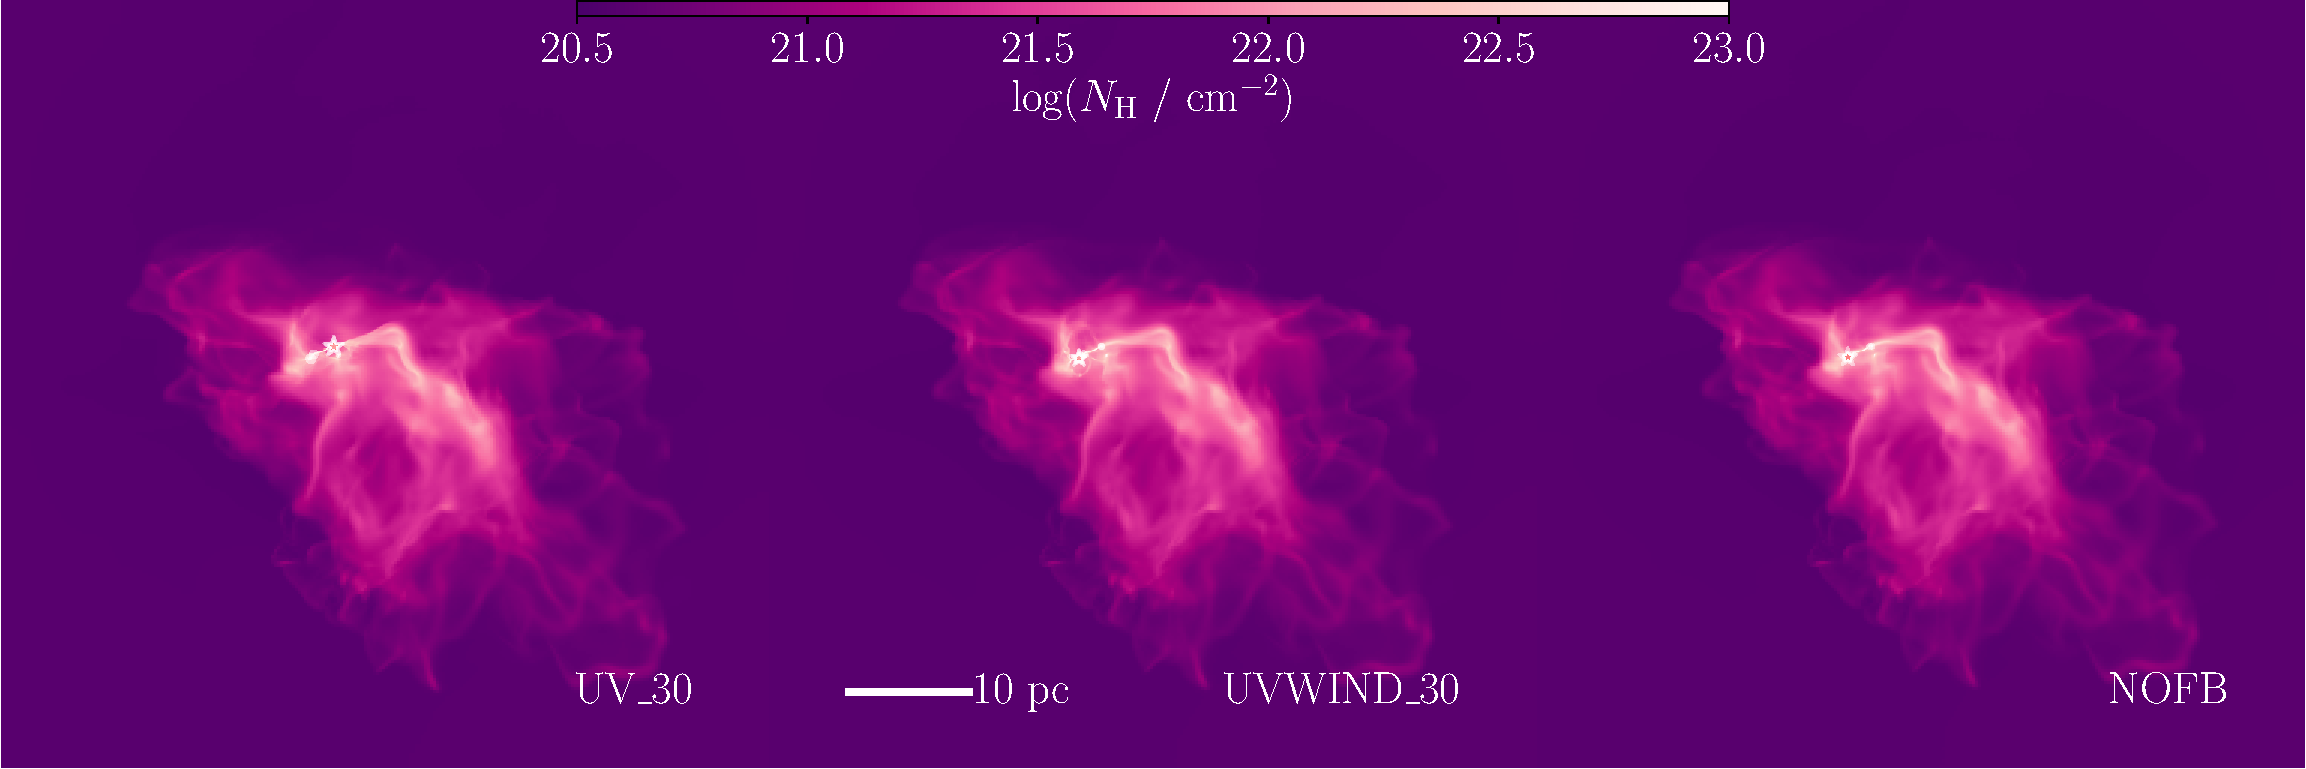
\includegraphics[width=2\columnwidth]{plots/fig1a.pdf}
	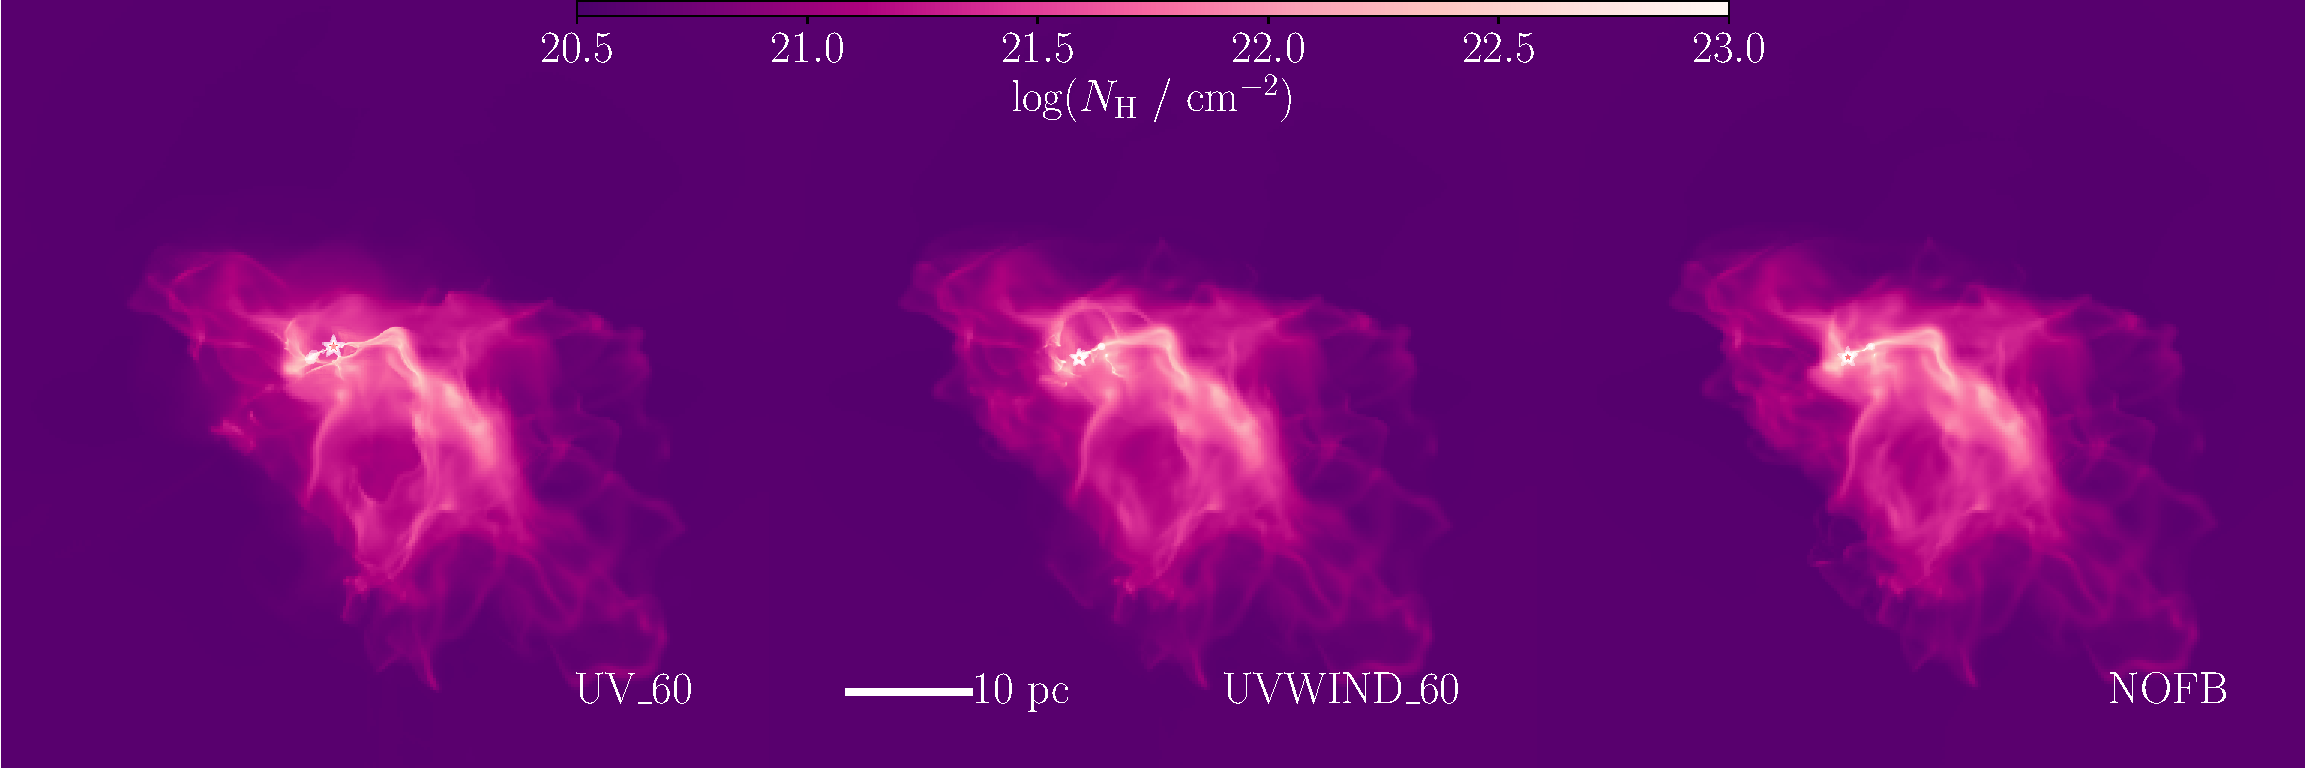
\includegraphics[width=2\columnwidth]{plots/fig1b.pdf}
	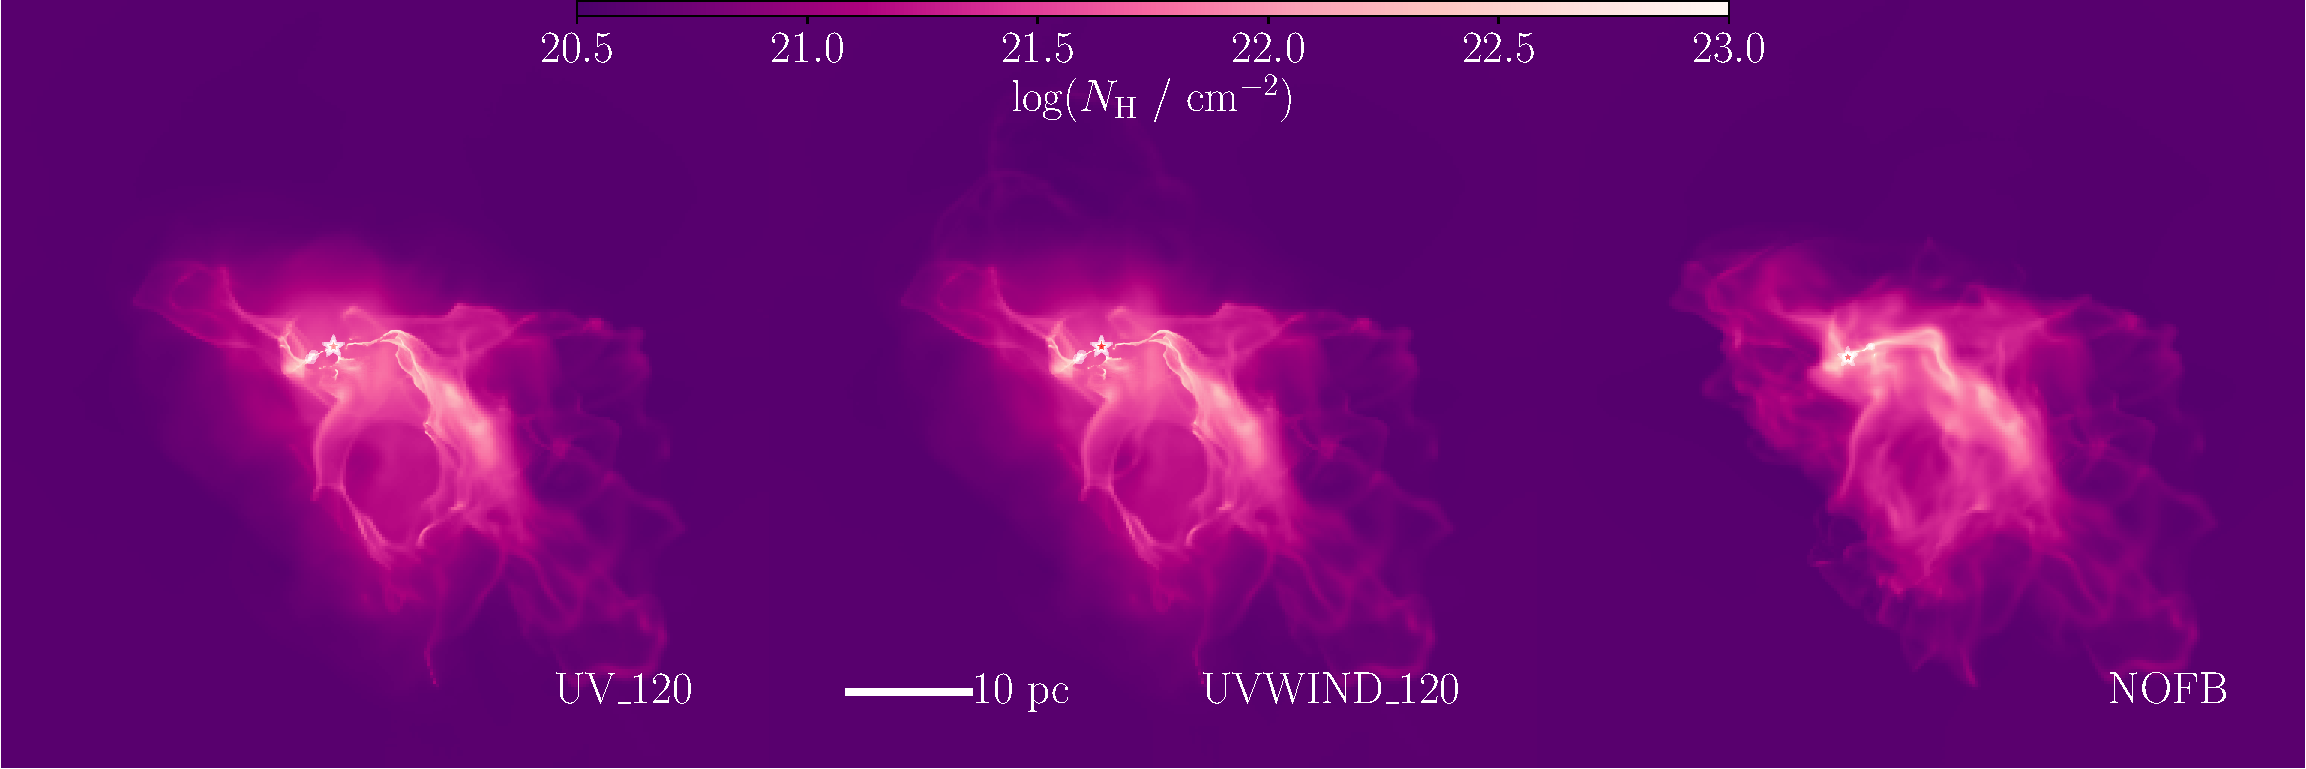
\includegraphics[width=2\columnwidth]{plots/fig1c.pdf}
	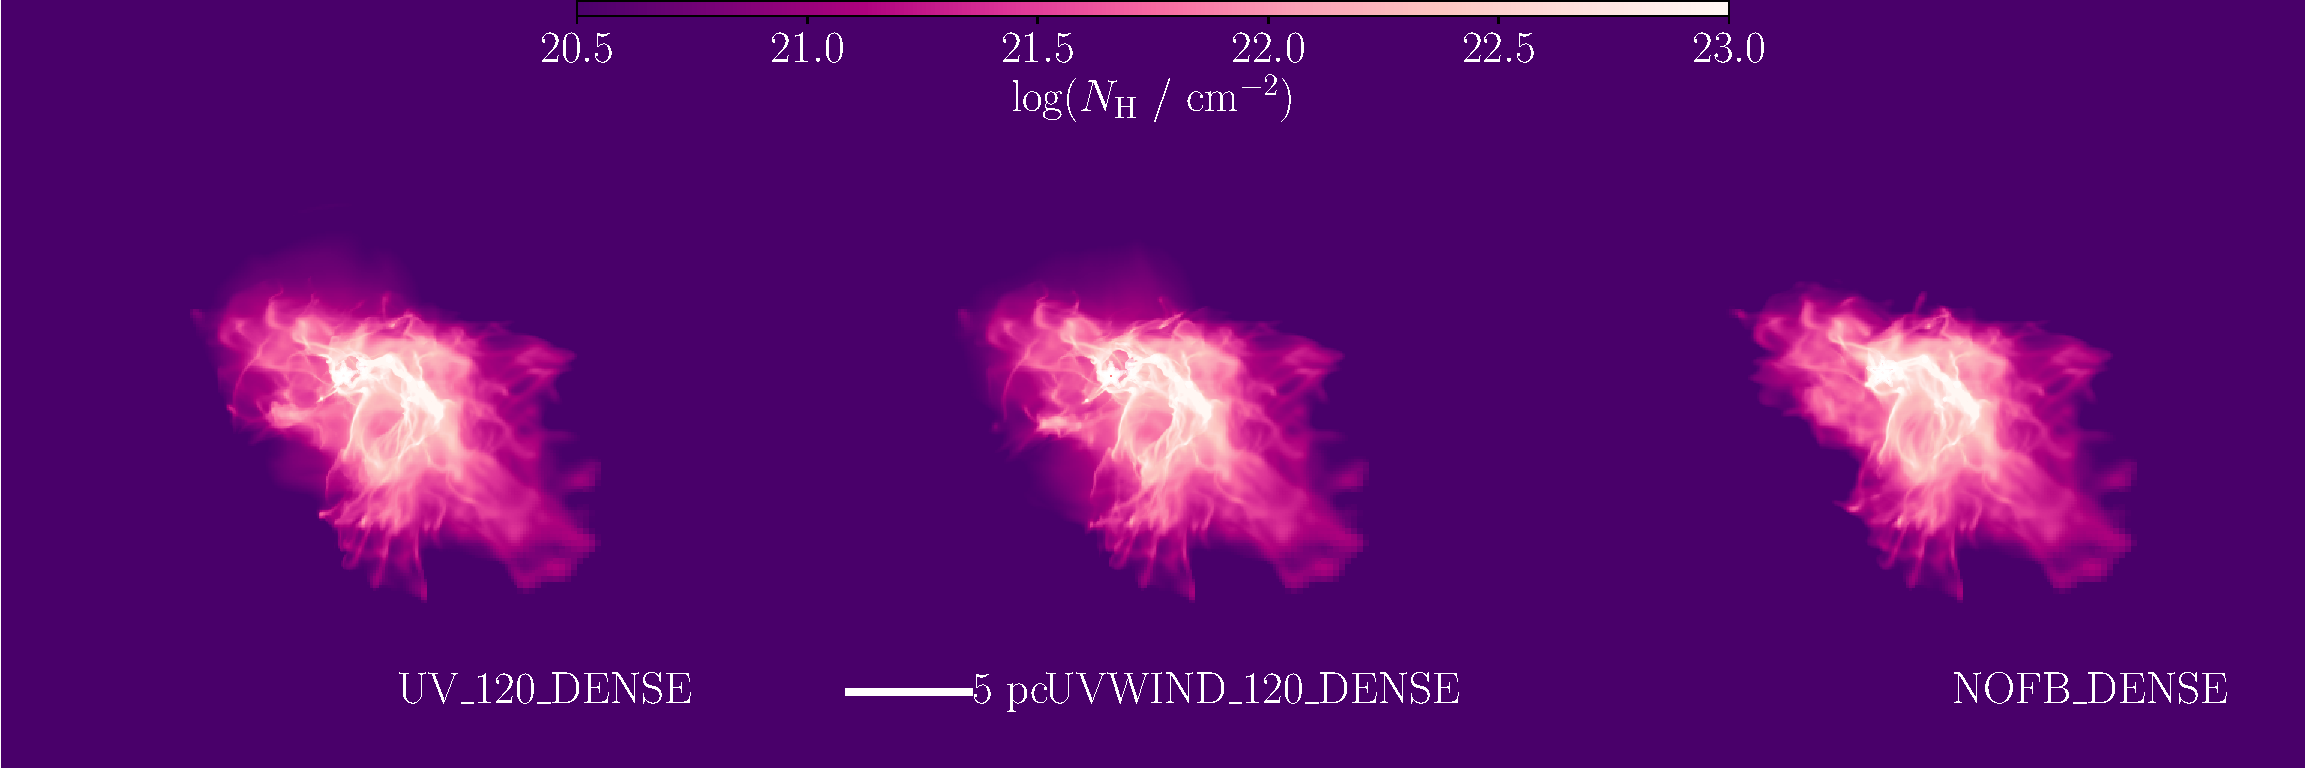
\includegraphics[width=2\columnwidth]{plots/fig1d.pdf}
	\caption{Column density maps of each simulation. From top to bottom we plot results for the 30 \Msolar star, the 60 \Msolar star, the 120 \Msolar star, and the 120 \Msolar star in the \textsc{dense} cloud. From left to right are simulations without feedback, simulations with just UV photoionisation and simulations with both UV photoionisation and winds.}
	\label{fig:columndensity}
\end{figure*}

In Figure \ref{fig:columndensity} we plot column density maps of each simulation at the same time relative to the freefall time of the cloud. In the 30 \Msolar cloud, there is evidence of an arc around the star where the \HII region is expanding. This bubble is larger when winds are included. In the 60 and 120 \Msolar star images below it, there is extended emission as the \HII region escapes the cloud and begins to evaporate the \textsc{dense} cloud gas. In the \textsc{dense} cloud containing a 120 \Msolar star in the bottom row, which is more compact, the cloud appears more fragmented while demonstrating similarly sized structures to the \textsc{diffuse} cloud.

%\begin{figure*}
%	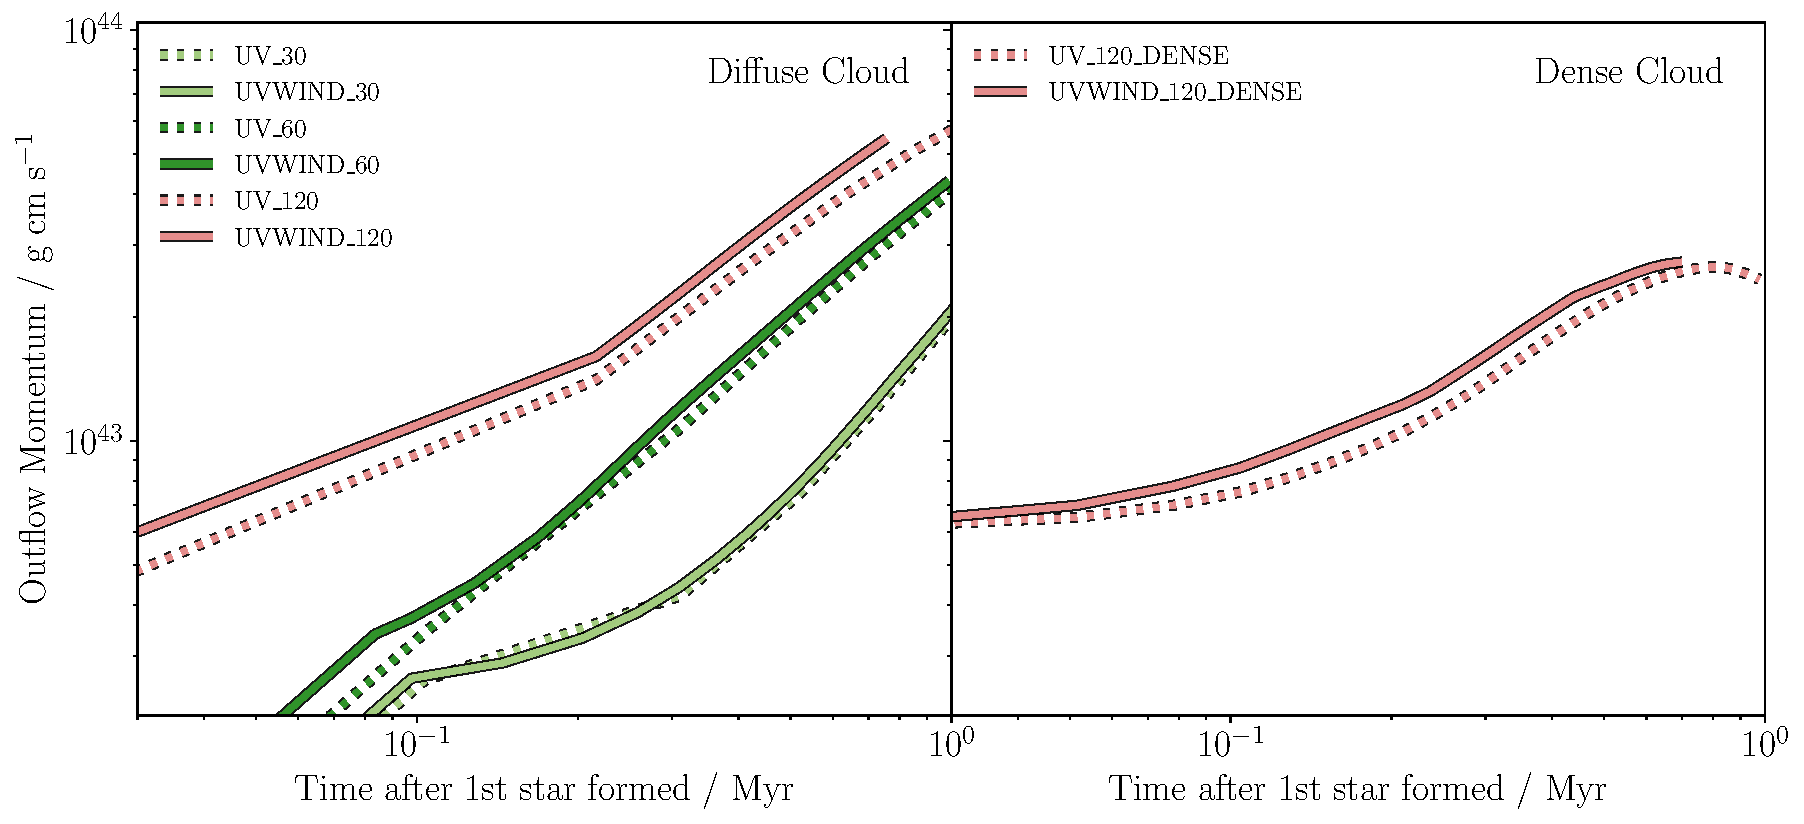
\includegraphics[width=2\columnwidth]{../plots/momentumatstarpos_both.pdf}
%	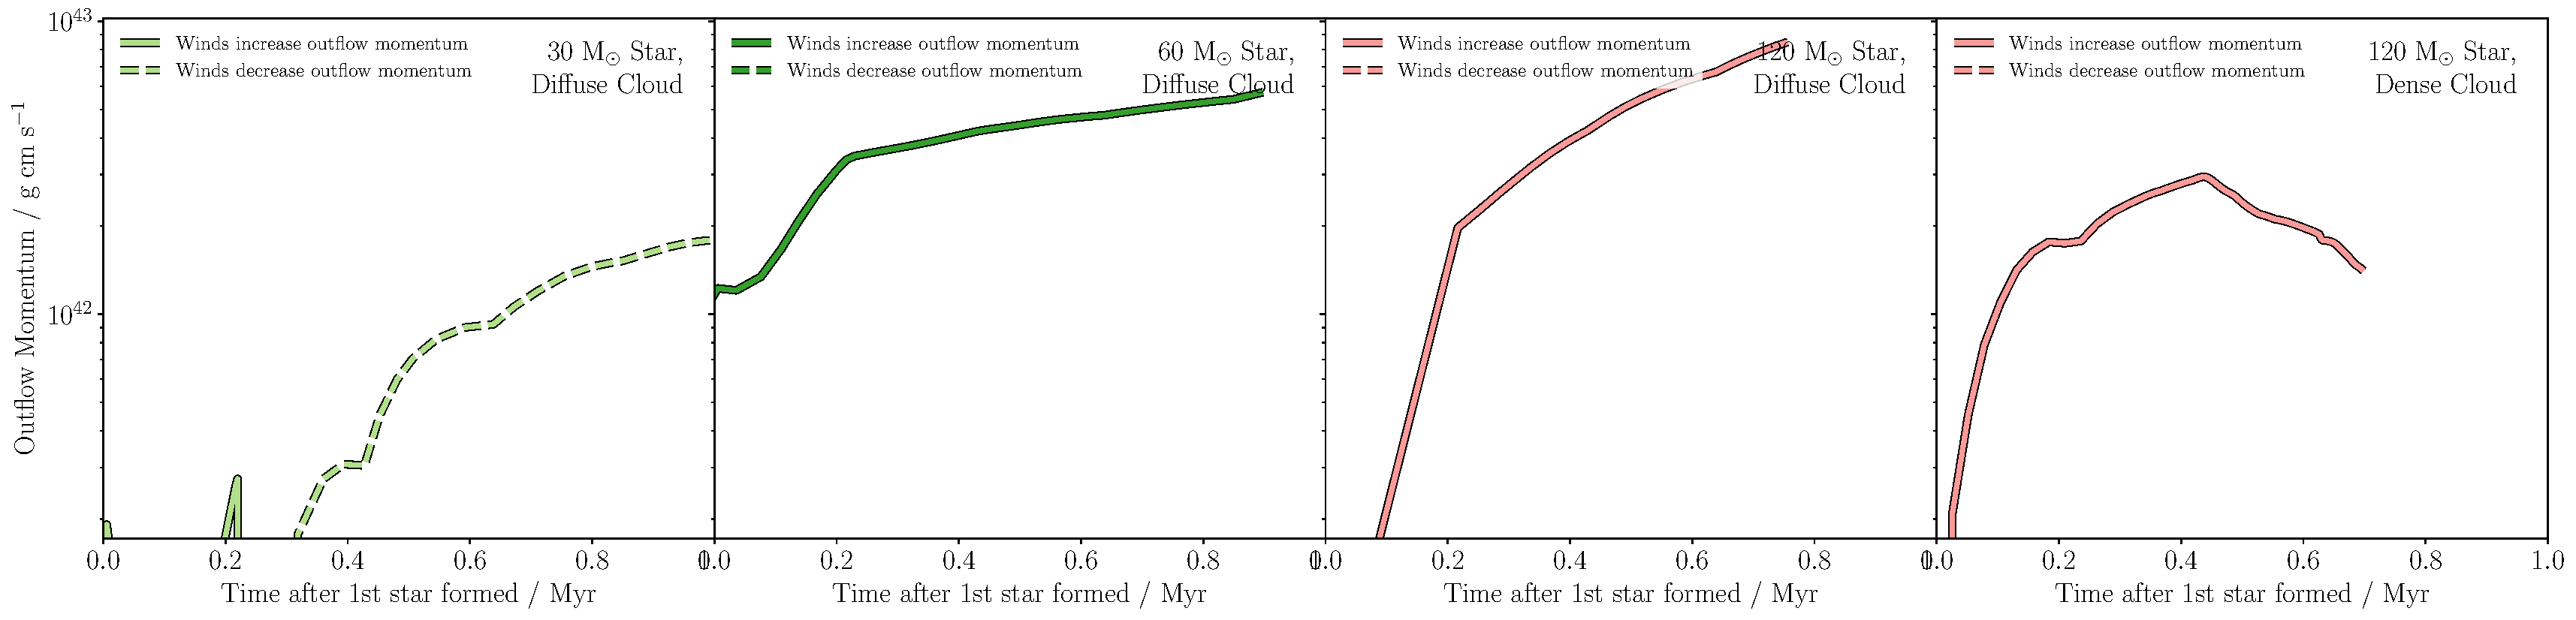
\includegraphics[width=2\columnwidth]{../plots/momentumatstarpos_both_compare.pdf}
%	\caption{Momentum injected in each simulation by the star. Top: Radial outwards momentum from the position of the star as a function of time in each simulation. Bottom: Difference in momentum between simulations including UV radiation with and without winds. A solid line indicates that the simulation including winds produces more momentum in outflows than an identical simulation without. A dashed line indicates that including winds produces less momentum.}
%	\label{fig:momentum}
%\end{figure*}

\begin{figure*}
	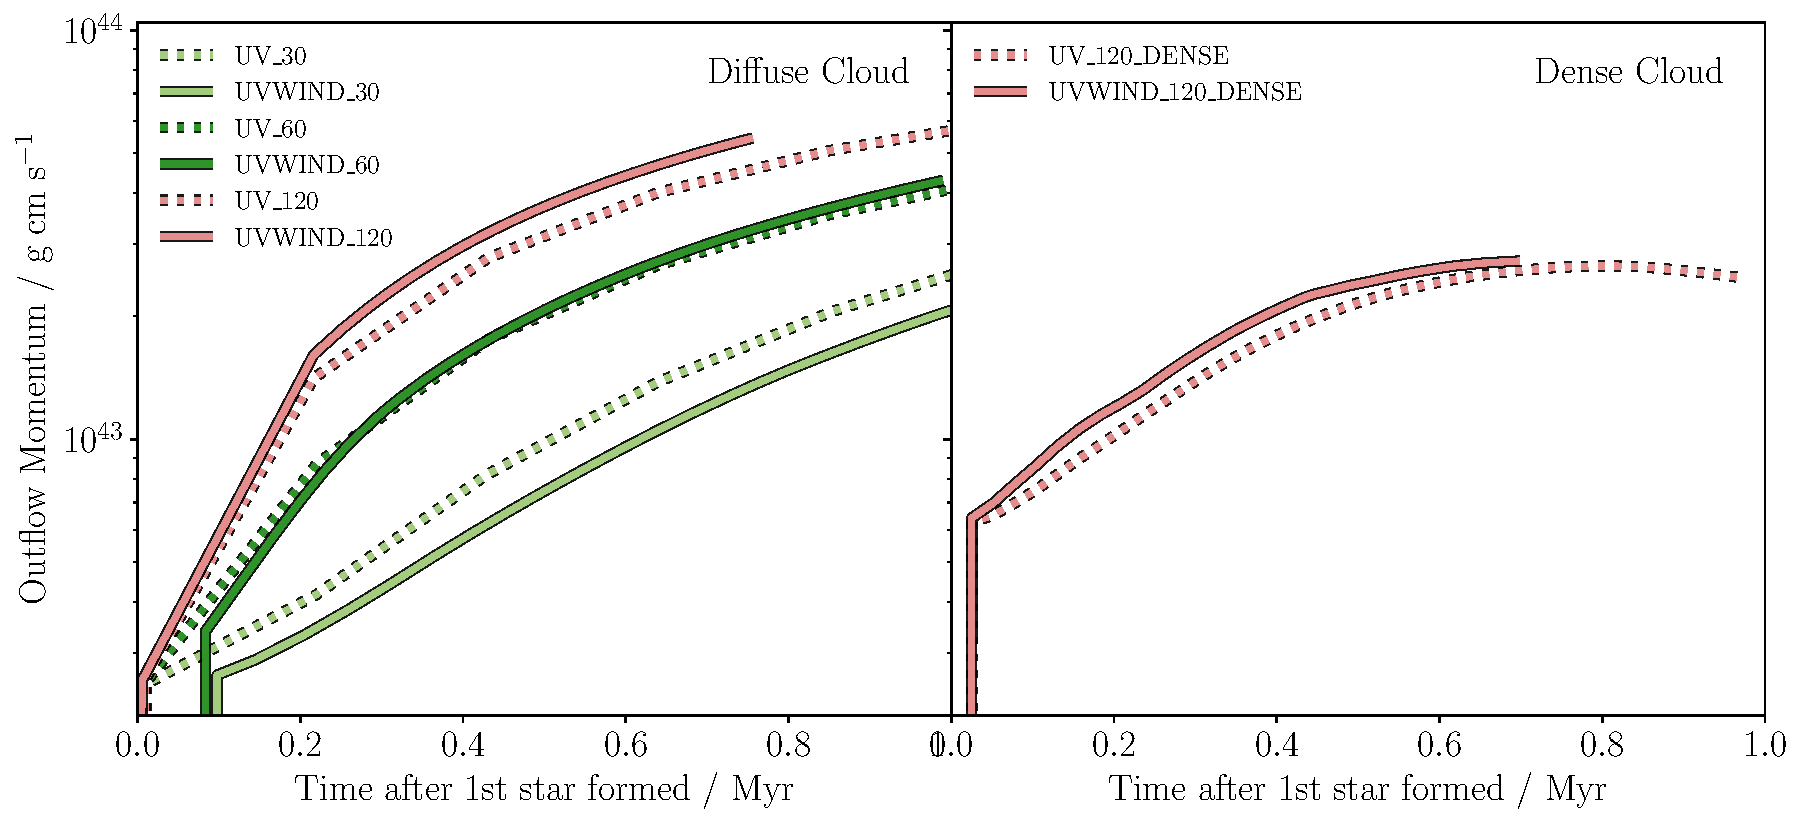
\includegraphics[width=2\columnwidth]{plots/fig2a.pdf}
	\caption{Radial outwards momentum from the position of the star as a function of time in each simulation. The gap between 0 and 0.1 Myr in some simulations is due to a) limited frequency of simulation outputs, and b) delay in feedback structures in resisting accretion flows.}
	\label{fig:momentum}
\end{figure*}

The momentum in outflows from the star in each simulation is shown in Figure \ref{fig:momentum}. In each case winds add approximately 10\% of the outflow momentum in the simulations containing just UV photoionisation. The exception is the 30 \Msolar star, which has a \textit{reduced} outflow momentum when winds are included. We posit that this is because UV photons are relatively inefficient at dispersing the cloud in this simulation. As a result, winds do more work in shaping the \HII region initially. This creates a dense shell, which absorbs the ionising photons efficiently, since recombination rates are proportional to $n^2$, where $n$ is the number density of atoms in the gas. In fully self-consistent simulations with multiple stars formed as in \cite{Geen2018}, we would expect to produce multiple stars if a single star is unable to end star formation in the cloud.

%\begin{figure*}
%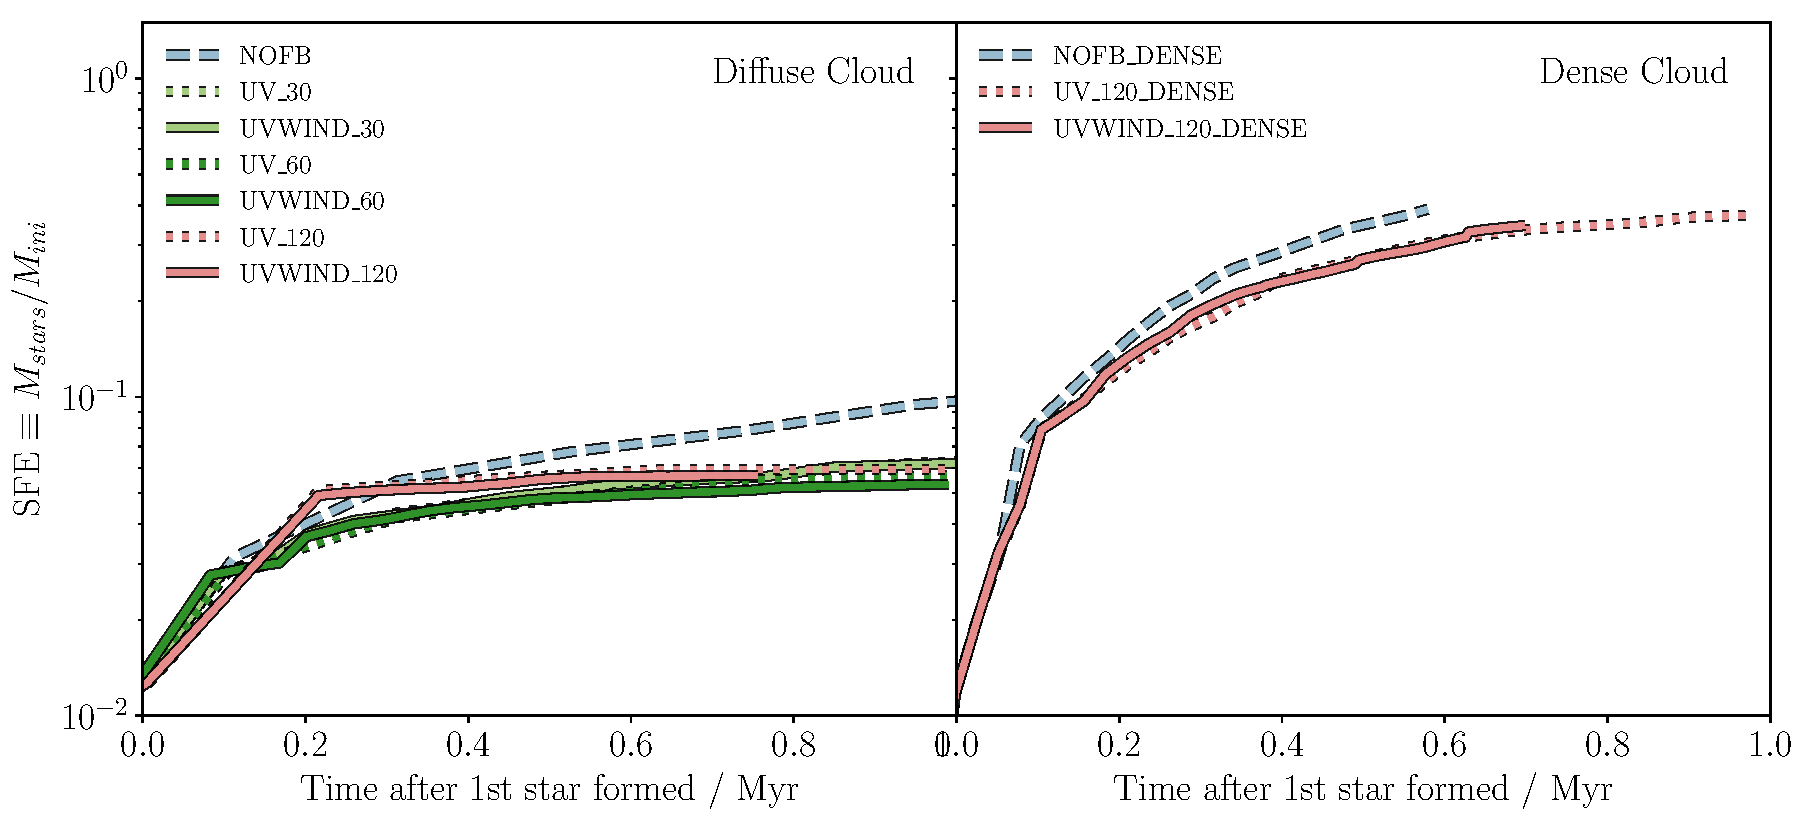
\includegraphics[width=2\columnwidth]{../plots/tsfe_both.pdf}
%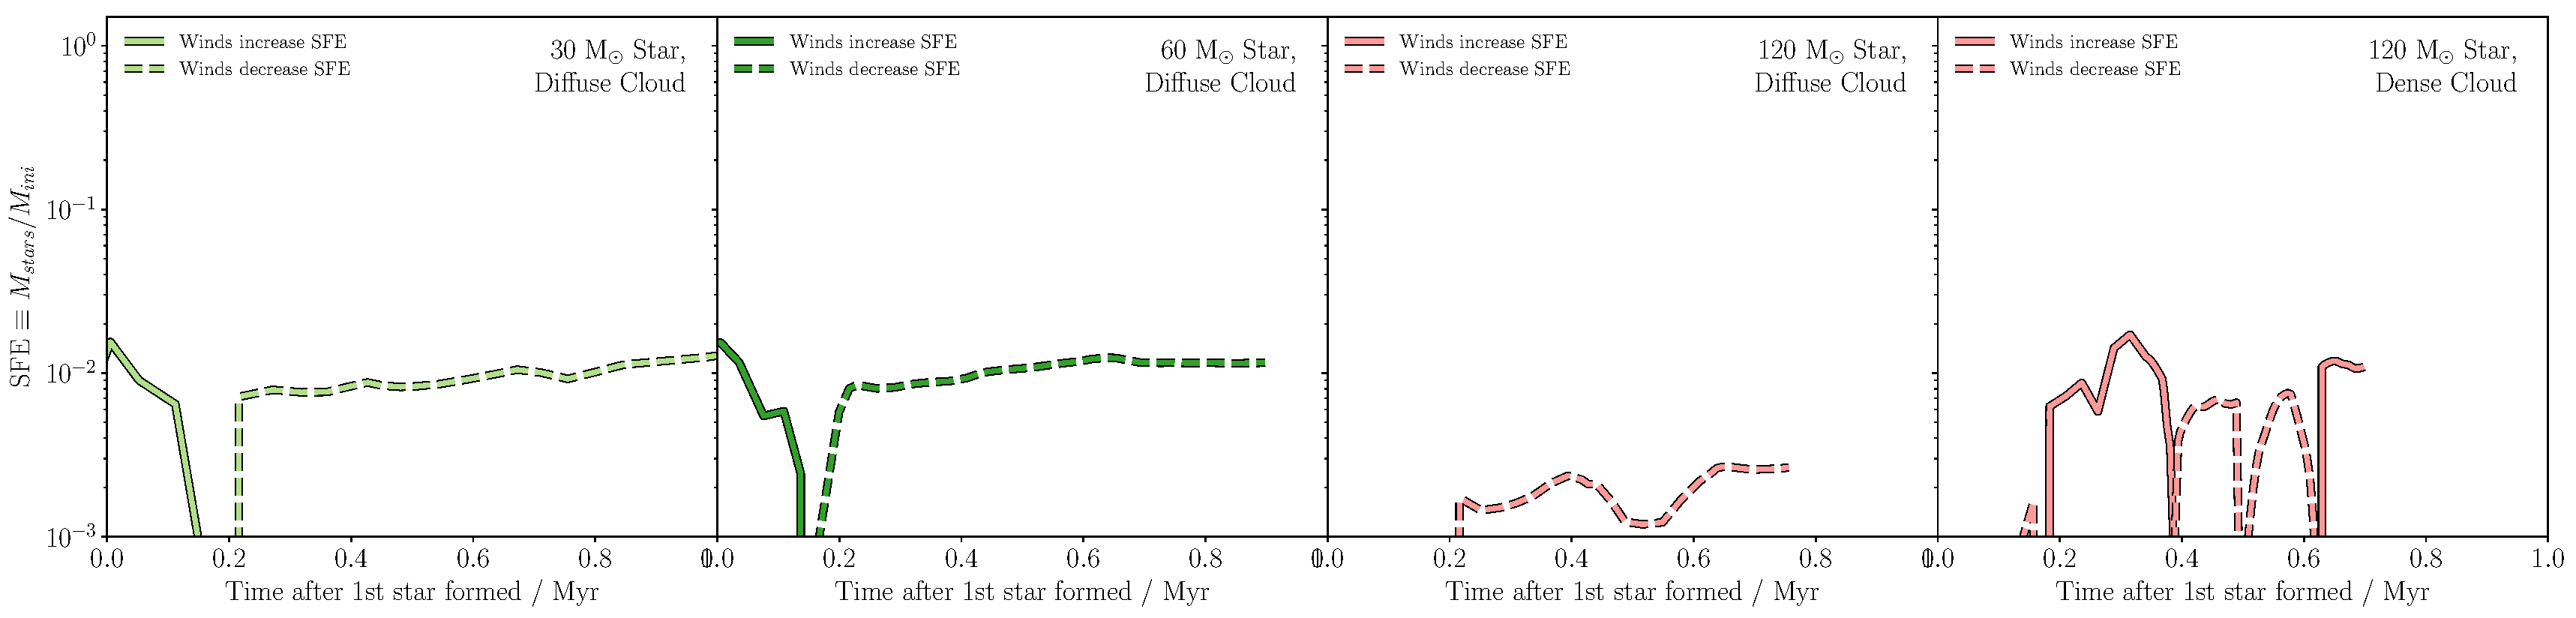
\includegraphics[width=2\columnwidth]{../plots/tsfe_both_compare.pdf}
%\caption{\protect\SFE, defined as the fraction of the initial gas mass converted to stars, in each simulation. Top: \protect\SFE as a function of time in each simulation. Bottom: Difference in \protect\SFE between simulations including UV radiation with and without winds. A solid line indicates that the simulation including winds produces more momentum in outflows than an identical simulation without. A dashed line indicates that including winds produces less momentum.}
%\label{fig:tsfe}
%\end{figure*}

\begin{figure*}
	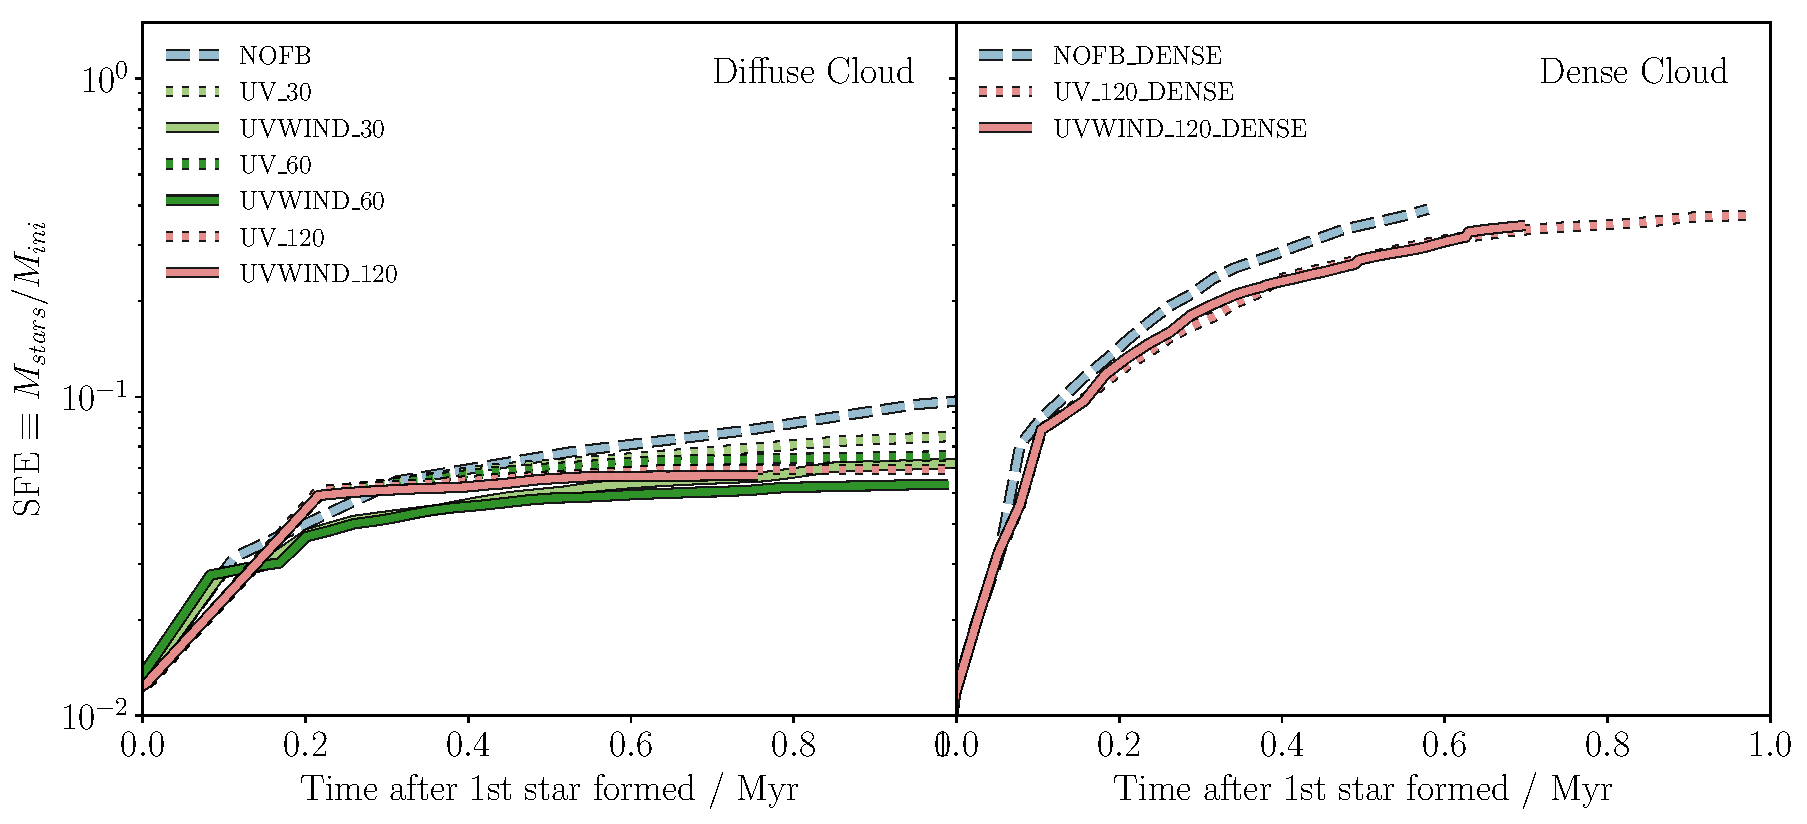
\includegraphics[width=2\columnwidth]{plots/fig3a.pdf}
	\caption{\protect\SFE, defined as the fraction of the initial gas mass converted to stars, as a function of time in each simulation.}
	\label{fig:tsfe}
\end{figure*}

Figure \ref{fig:tsfe} shows the \SFE of the cloud in terms of fractional mass in gas in the cloud converted to stars (referred to as \TSFE in \cite{Geen2017}, \cite{He2019} and others). In the simulations containing 30 and 60 \Msolar stars, winds reduce \SFE in the first Myr by approximately 10\% compared to simulations with just UV photoionisation. The boost to \SFE in the initial 100 kyr could be due to compression from the winds, but it is also possibly due to the time that simulation outputs are taken in each simulation. In simulations with 120 \Msolar stars in both the \textsc{diffuse} and \textsc{dense} clouds, it is not clear whether winds have a significant effect or not on \SFE.

Broadly, winds have at best a 10\% effect on these bulk properties during the first Myr of the star's life. We now look in more detail at the evolution and energetics of the wind bubble in particular.

\subsection{The Evolution of the Embedded Wind Bubble}
\label{results:evolutionwindbubble}

\begin{figure*}
	\centerline{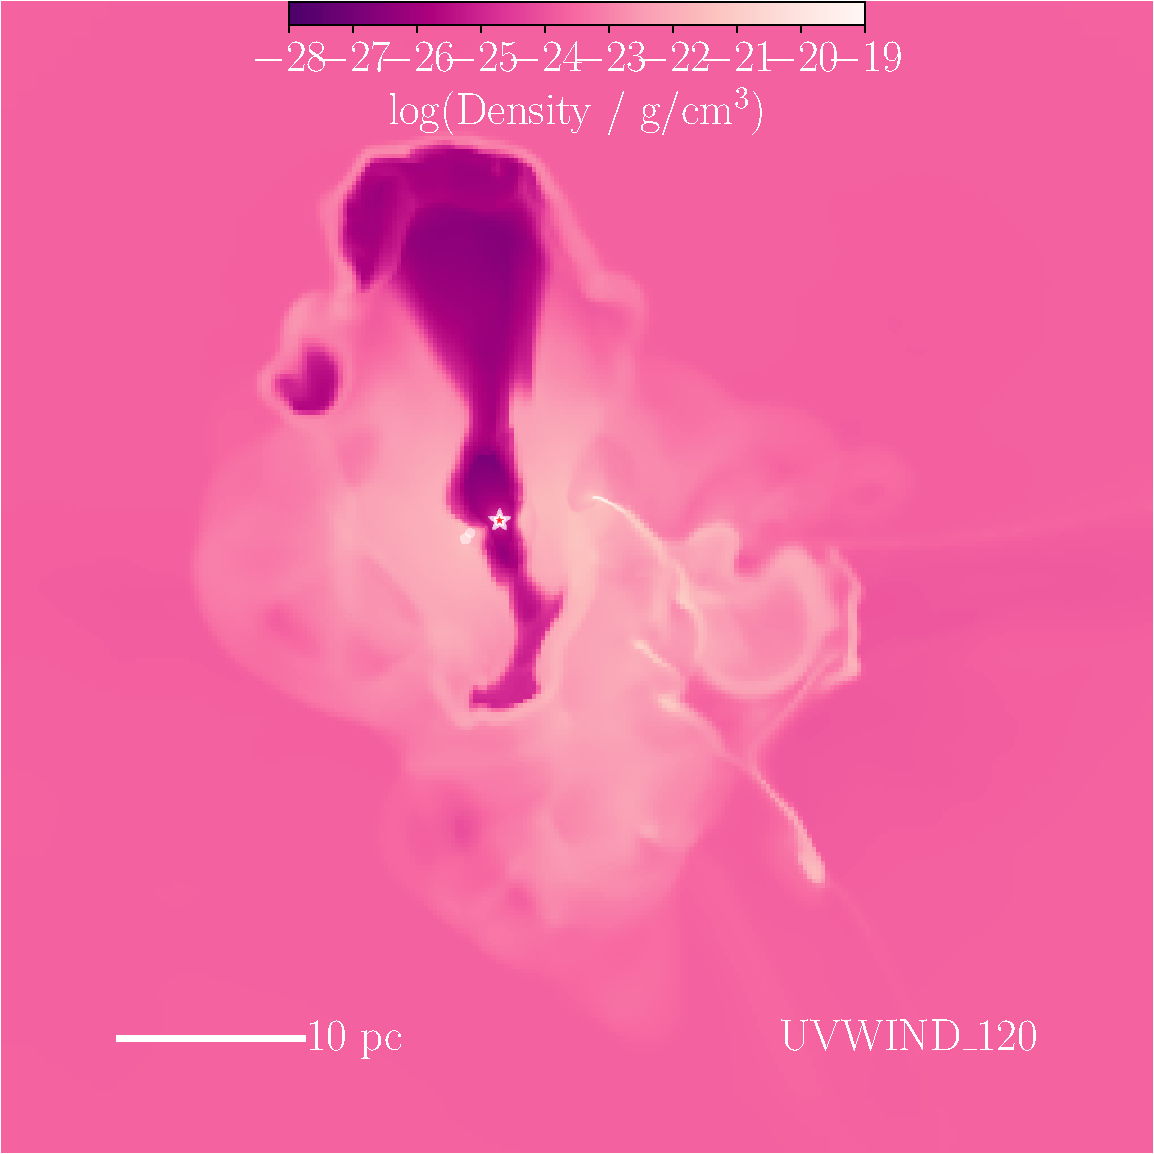
\includegraphics[width=0.80\columnwidth]{plots/fig4a.pdf} 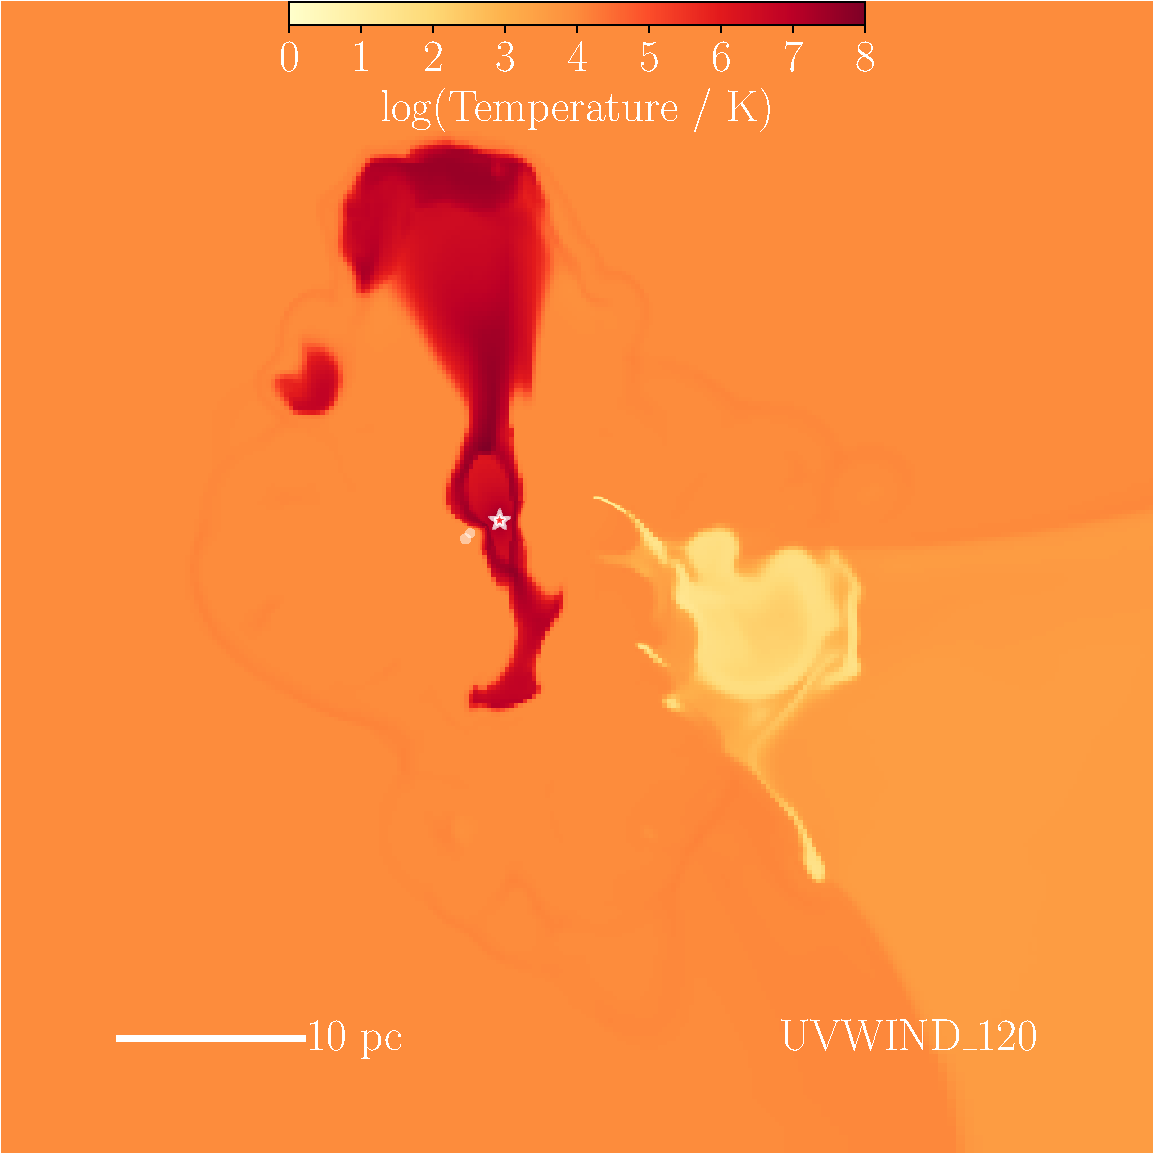
\includegraphics[width=0.80\columnwidth]{plots/fig4b.pdf}}
	\centerline{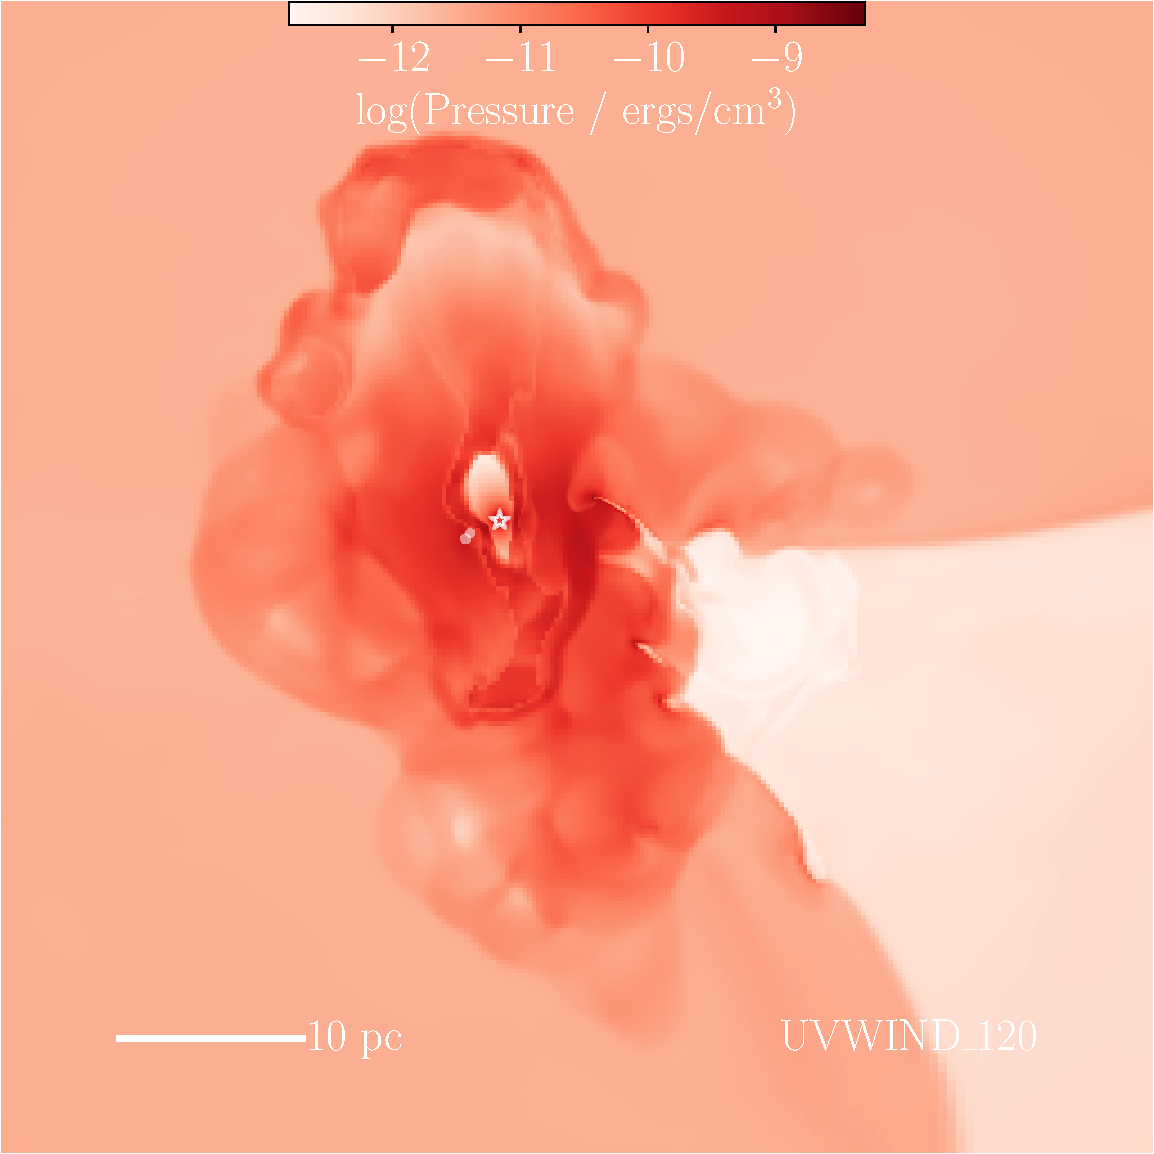
\includegraphics[width=0.80\columnwidth]{plots/fig4c.pdf}
	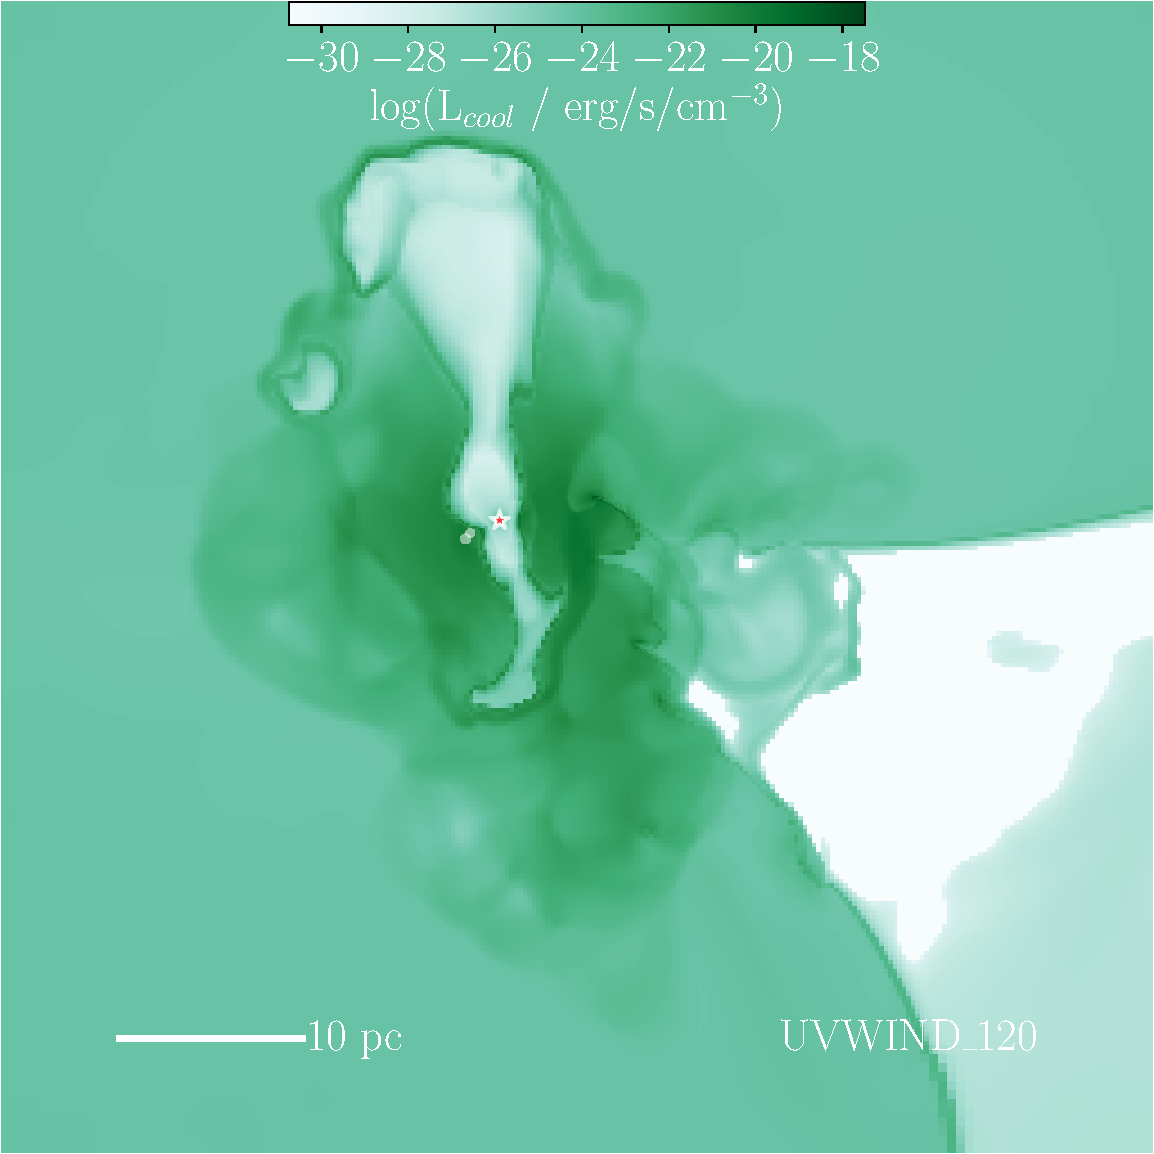
\includegraphics[width=0.80\columnwidth]{plots/fig4d.pdf}}
	\caption{Slices through the simulation volume in the UV120 simulations, showing various properties of the gas. The images are shown in the y-axis of the Cartesian volume, with the slice taken through the y position of the star. Each image is 61 pc on-a-side, i.e. half of the total box length. From top left to bottom right, we plot mass density, temperature, thermal pressure and cooling rate (as luminosity per unit volume). The positions of sink particles are shown as white dots. The low pressure region to the right is the shadow behind the remaining neutral gas in the cloud. Most of the simulation volume is already photoionised.}
	\label{fig:windslices}
\end{figure*}

\subsubsection{Overview}
\label{results:evolutionwindbubble:overview}

To illustrate the internal structure of the wind bubble in the 120 \Msolar case, we show slices through the \HII region in Figure \ref{fig:windslices}. The plane of the slice is set at the y position of the star. The structure of the bubble agrees in qualitative terms with the schematic presented in \cite{Weaver1977}. However, the geometry of the wind is very different.

Once the bubble has reached a sufficient pressure, it is able to punch through the now photoionised cloud and escape into the surrounding medium. The bubble has two structures, 1) a conical \textit{chimney} extending from the star upwards into lower-pressure gas and 2) above the chimney, an extended \textit{plume} that expands into the lower-density background.

\subsubsection{Interaction with the Photoionised Region}
\label{results:evolutionwindbubble:interaction}

The entire bubble has a lower density than the surrounding photoionised region since it has a higher temperature while retaining pressure equilibrium. Around the star is a free-streaming region that is a largely kinetic outflow. The initial temperature of the wind is high since the wind should be ionised due to interaction with stellar radiation. However, the temperature is also elevated due to self-shocking as a numerical consequence of placing spherical flows onto a Cartesian grid. This artefact can be reduced but not entirely mitigated, although we note that as long as the flow remains adiabatic and largely kinetic, its importance is negligible.

Outside of this region, the free-streaming wind shocks against the background, creating a hot bubble of $10^7$ to $10^8$ K, where it is in pressure equilibrium with the photoionised gas. 

The majority of the simulated volume is at this point photoionised by rapid ``champagne'' flows \citep{Bodenheimer1979,TenorioTagle1979,Whitworth1979}, and the temperature of the photoionised gas achieves a roughly constant equilibrium temperature of around $10^4$ K. The cloud at this point follows the mode described in \cite{Franco1990} where the expansion of the cloud is driven by a pressure difference created by the remaining density gradient in the cloud. This occurs at a few times the speed of sound in the ionised gas ($\sim 30$ km/s).

\subsubsection{Transition between Phases}
\label{results:evolutionwindbubble:phases}

Since the temperature of wind is around $10^4$ times that of the photoionised gas, its sound speed is approximately 100 times faster. This creates a much faster flow that seeks pressure equilibrium by following the density gradient in the photoionised cloud. In simulations using the 30 \Msolar star, this bubble is elongated but mostly contained within the cloud. With the 120 \Msolar star, the winds have sufficient luminosity to create the chimney-and-plume structure.

The cooling inside the wind bubble is much lower than its surroundings. Most of the cooling in the wind bubble occurs at the interface between the wind and the surrounding medium. The energy losses from the photoionised gas are considerably higher due to the large amount of energy lost to recombination \citep[see the analysis by][]{Walch2012}. 

The plume phase does not have to have a corresponding chimney phase. The hot chimney can be cut off temporarily if a dense flow interacts with the wind, leaving a cut-off plume. The chimney will re-establish itself shortly after. This gives the impression of the wind bubble reaching radii towards the edge of the bubble without it actually interacting with gas closer to the star. We show examples of this happening in the \textsc{dense} cloud in the following sections.

\subsection{The Energetics of the Embedded Wind Bubble}
\label{results:energeticswindbubble}

\begin{figure*}
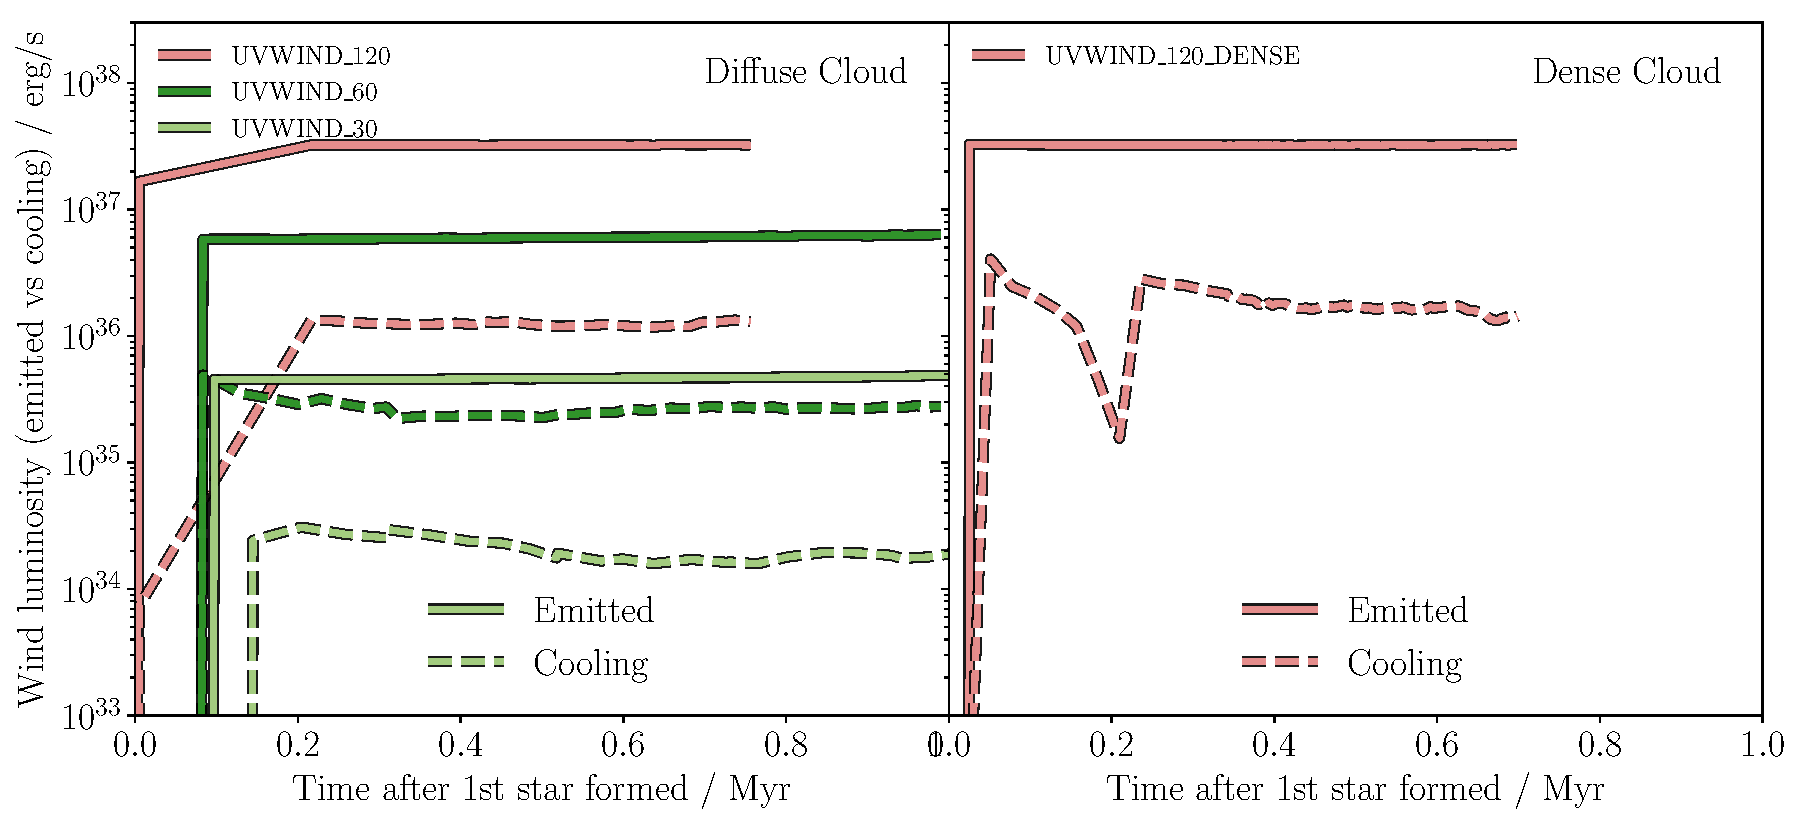
\includegraphics[width=1.98\columnwidth]{plots/fig5a.pdf}
\caption{Wind luminosity (solid line) versus rate of energy loss to radiative cooling in the wind bubble (dashed line) as a function of time in each simulation containing winds. The wind bubble is identified as gas that is above 100 km/s or $10^5$ K (see Section \protect\ref{results:energeticswindbubble}). Emitted luminosity values are sampled from the stellar evolution tables (see Section \protect\ref{methods}) for the star's age at each timestep in the simulation. The gap from 0 to 0.1 Myr is due to limited frequency of simulation outputs. There is a further delay in cooling in UVWIND\_30 due to the time taken to heat the cells around the star to above $10^5$ K.}
\label{fig:windLemittedvscool}
\end{figure*}

In Figure \ref{fig:windLemittedvscool} we plot the wind luminosity emitted by the star versus the energy lost to radiative cooling as a function of time in the wind bubble. We identify cells as being in the wind bubble if they are either a) hotter than $10^5$ K or b) contain flows faster than 100 km/s with respect to the static reference frame. The cooling rate inside the wind bubble is, as shown in Figure \ref{fig:windslices}, only a few percent of the emitted wind luminosity. As shown in Figure \ref{fig:windslices}, most of the energy is lost in mixing with the denser gas around it. We thus do not expect a large fraction of the wind luminosity to be lost to radiative cooling via hot x-ray emission, but rather lower energy bands. The observability of this is complicated by the fact that there will be significant emission already from recombination in the photoionised \HII region, masking the losses from winds.

As second mode found in \cite{Rogers2013} and \cite{Dale2014}, the ablation of dense clumps trapped inside the wind bubble, does not appear to be significant, since we do not model multiple wind sources that could create such trapped clumps. However, we do observe an additional process temporarily affecting the cooling rate in the \textsc{dense} cloud. The wind source is temporarily quenched by dense gas flows around the massive star, analogous to the ``flickering'' of \HII regions observed by \cite{Peters2010}. This cuts off the wind chimney and leaves an isolated plume. This event is only temporary, and the whole event lasts only around 200 kyr.

\begin{figure*}
	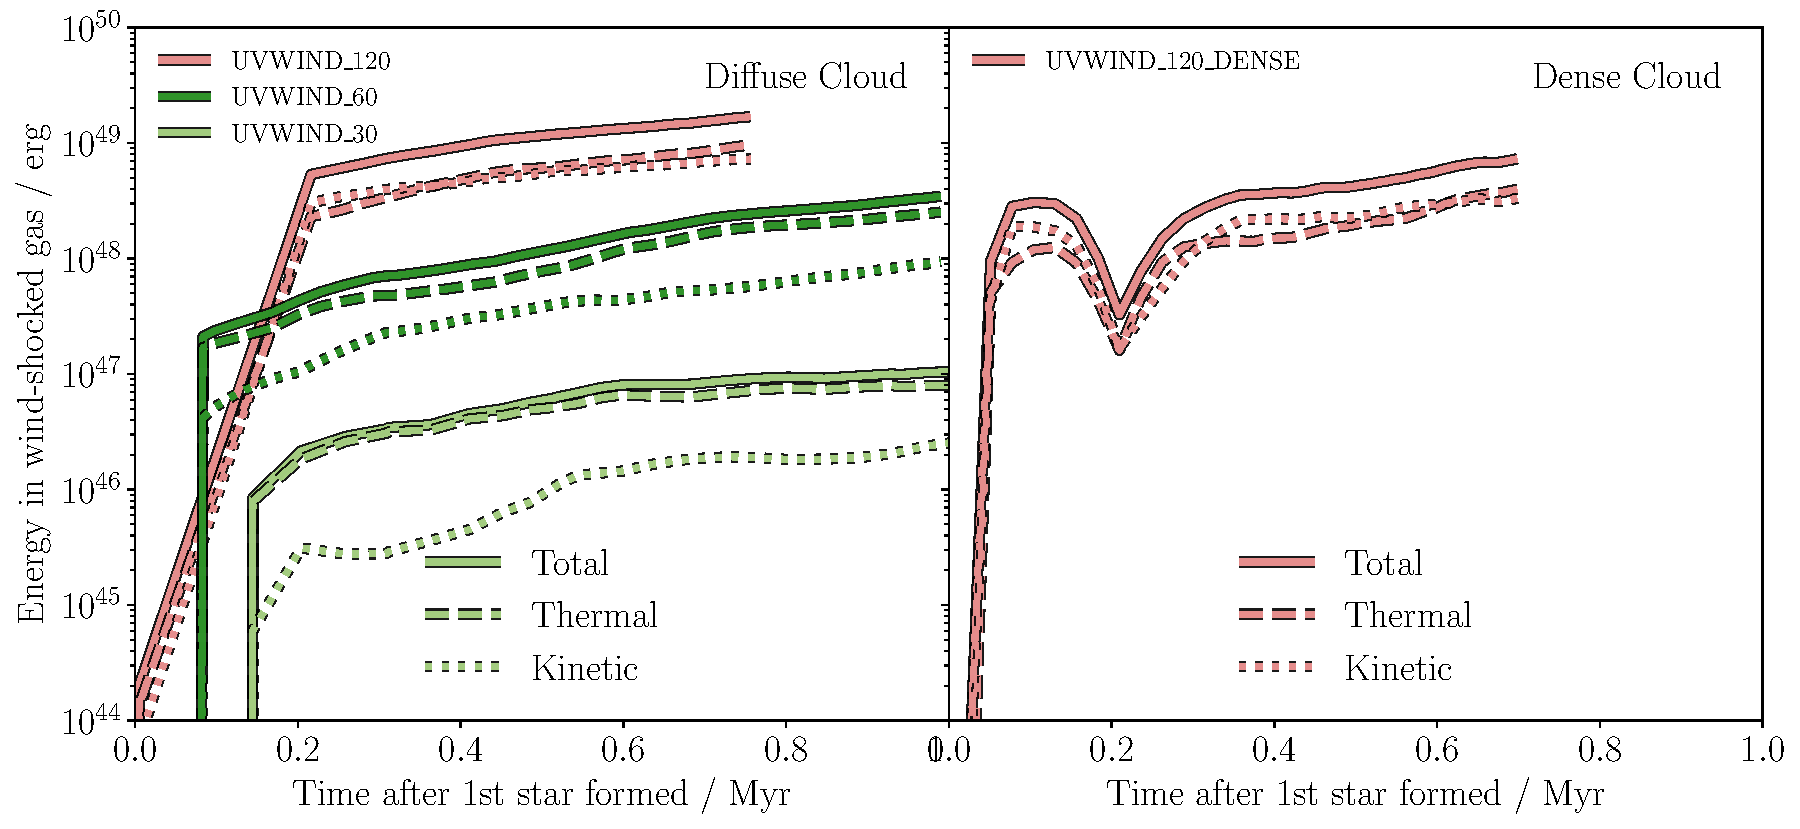
\includegraphics[width=1.98\columnwidth]{plots/fig6a.pdf}
	\caption{Energy in the wind bubble as a function of time in each simulation containing winds, showing kinetic energy (dotted line), thermal energy (dashed line) and the total of the two (solid line). The wind bubble is identified as gas that is above 100 km/s or $10^5$ K (see Section \protect\ref{results:energeticswindbubble}).}
	\label{fig:windenergy}
\end{figure*}

As discussed in Section \ref{results:evolutionwindbubble}, the wind bubble is divided into a free-streaming region driven by fast flows, and a shocked, thermalised region. In Figure \ref{fig:windenergy}, the 30 and 60 \Msolar stars produce a bubble that is largely thermalised, shown by the smaller quantity of kinetic energy compared to thermal energy. In the bubbles around the 120 \Msolar star in both the \textsc{diffuse} and \textsc{dense} clouds, there is a rough equipartition of energy, with the \textsc{dense} cloud even exhibiting more kinetic than thermal energy in the wind bubble at times.

\begin{figure*}
	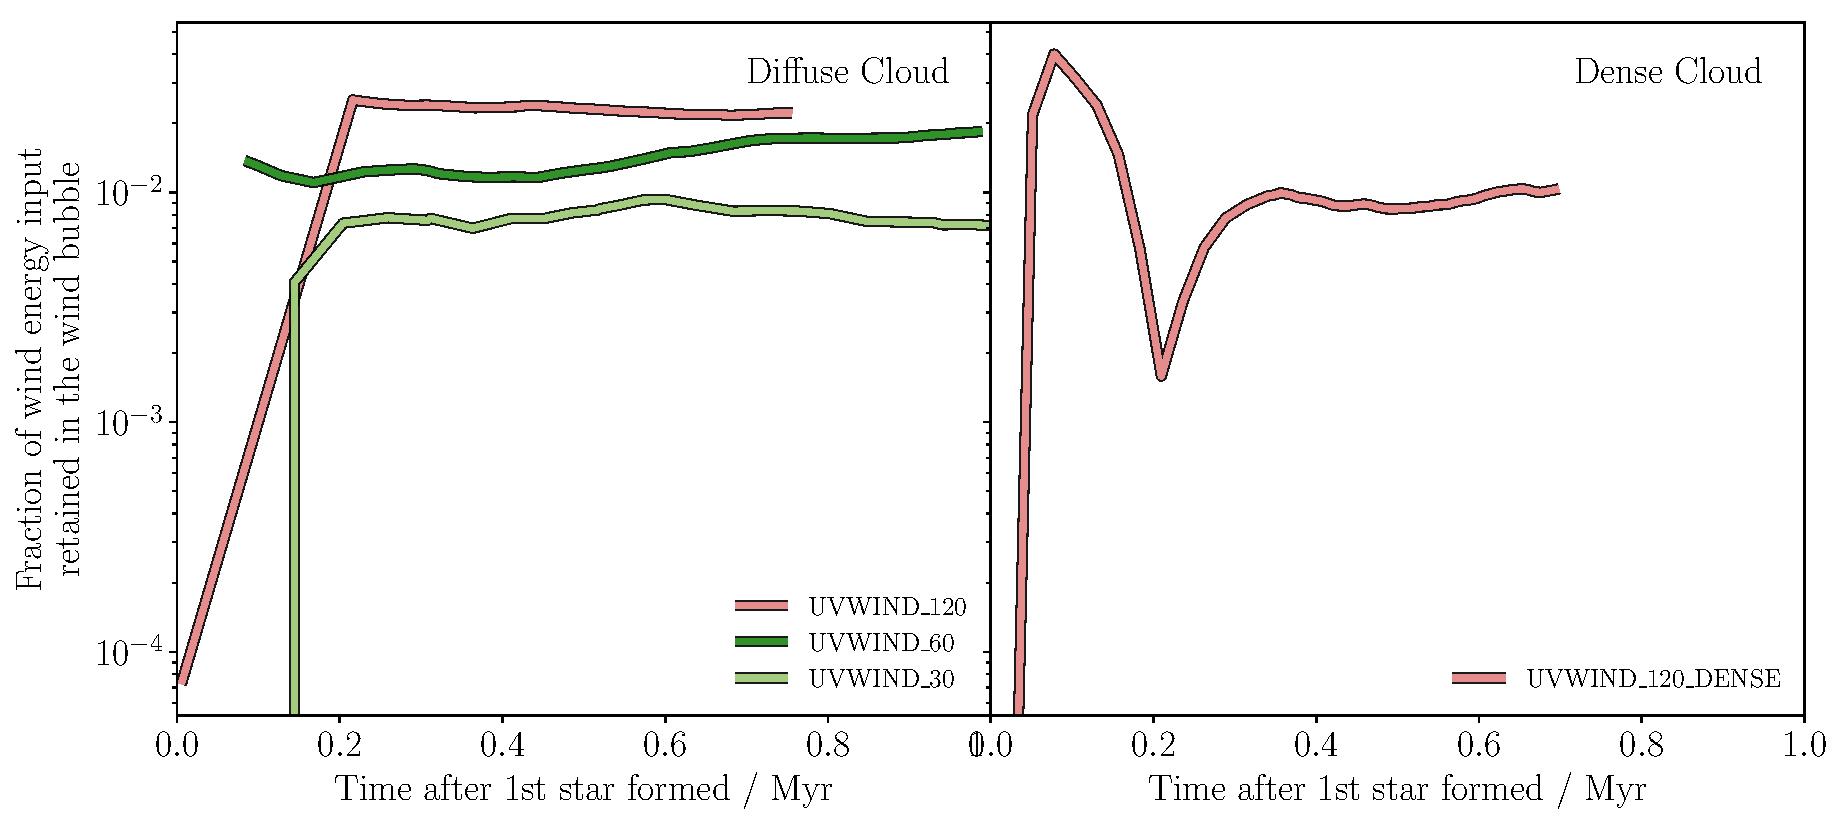
\includegraphics[width=1.98\columnwidth]{plots/fig7a.pdf}
	\caption{Fraction of energy emitted by stellar winds retained in the wind bubble as a function of time for each simulation containing winds. The wind bubble is identified as gas that is above 100 km/s or $10^5$ K (see Section \protect\ref{results:energeticswindbubble}).}
	\label{fig:windenergyretained}
\end{figure*}

Approximately 1\% of the energy emitted by the star is retained in the wind bubble, as shown in Figure \ref{fig:windenergyretained}. More energy is retained the more massive the star is. 

Note that this ignores any energy transferred to the gas outside the wind bubble. However, since the speeds in this gas are typically lower, kinetic energy will be higher inside the bubble. Similarly, given the high cooling rates outside the bubble, we posit that most of the energy transferred to the gas outside the bubble is lost to cooling.

\begin{figure*}
	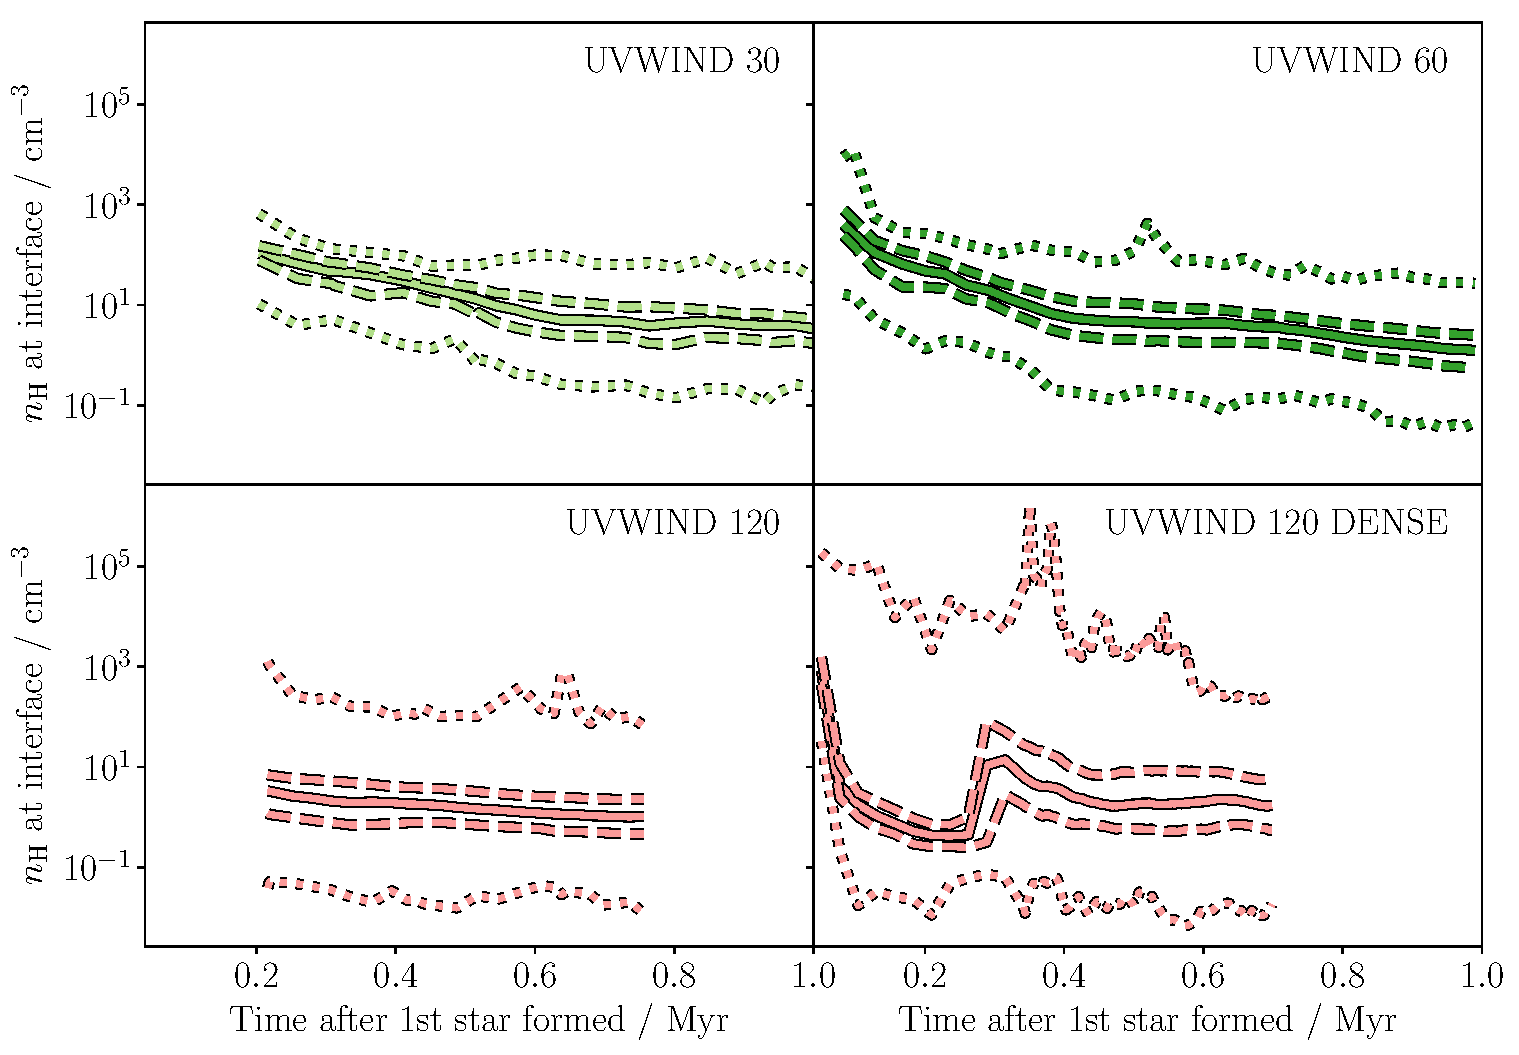
\includegraphics[width=1.98\columnwidth]{plots/fig8a.pdf}
	\caption{Distribution of densities on the interface between the wind bubble and the gas outside as a function of time in each simulation that includes stellar winds. The median density is shown as a solid line. The minimum and maximum densities are shown as dotted lines. Dashed lines show the interquartile range (capturing 50\% of the distribution).}
	\label{fig:findHIIdensities}
\end{figure*}

\begin{figure}
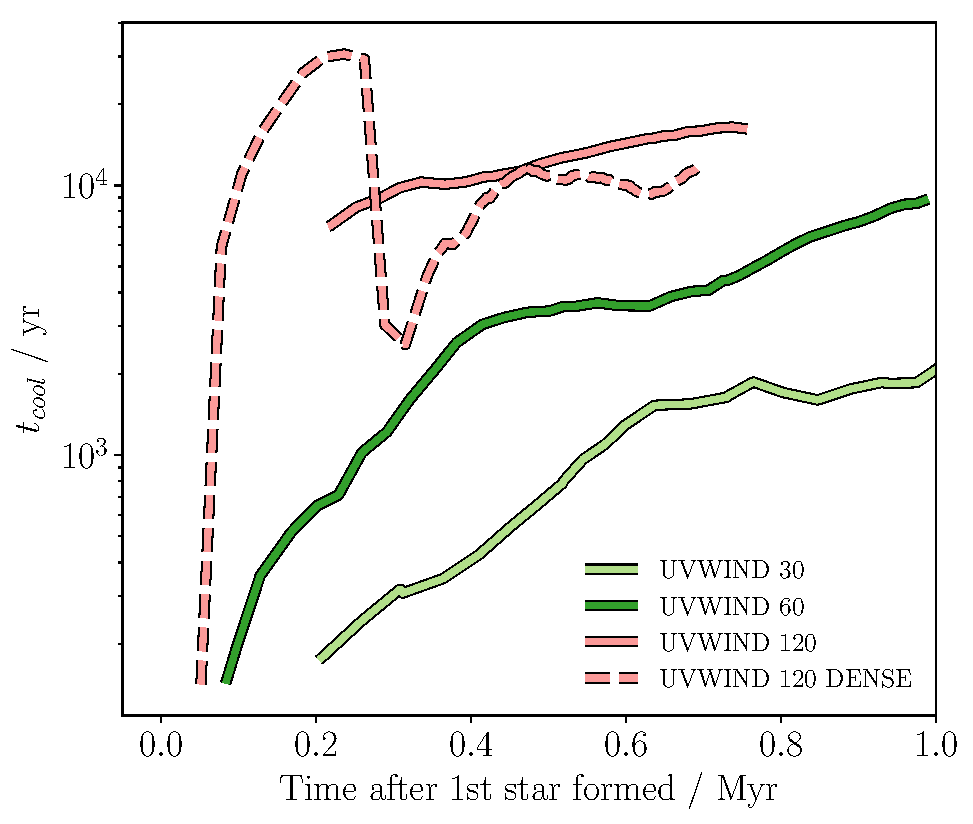
\includegraphics[width=0.98\columnwidth]{plots/fig9a.pdf}
\caption{Estimated cooling time $t_{cool}$ of the wind bubble as a function of time in each simulation containing winds. The cooling time is calculated using Equation \ref{equation:tcool}. The external density $n_0$ is taken to be the median density plotted in Figure \ref{fig:findHIIdensities}, and the wind luminosity is taken from the stellar evolution tables. See Section \ref{results:energeticswindbubble} for a discussion of this calculation and some caveats.}
\label{fig:coolingtimes}
\end{figure}

\cite{MacLow1988} use \cite{Cowie1977}'s spherical evaporation model to quantify the cooling of a wind bubble based on mass evaporation from the surface of the bubble. They give a cooling time $t_c$ of
\begin{equation}
t_c = (2.3 \times 10^4 \mathrm{yr}) n_0^{-0.71} L_{38}^{0.29}
\label{equation:tcool}
\end{equation}
where $n_0$ is the density of the ambient medium around the wind bubble and $L_{38}$ is the wind luminosity in units of $10^{38}$ erg/s. The total cooling rate is an inverse function of $t_c$. In other words, cooling becomes more efficient with higher external density and less efficient with higher wind luminosities. \cite{MacLow1988} also include a model for the cooling of the bubble itself, which we have established is relatively inefficient in our simulations.

 In Figure \ref{fig:findHIIdensities}, we plot the distribution of densities around the wind bubble as a function of time. In Figure \ref{fig:coolingtimes} we use the median density to plot $t_{cool}$ as a function of time in each simulation. Note that this is a very rough estimate of the cooling time - it ignores factors such as the geometry and expansion rate of our cooled bubble.
 
 In all of our simulations, $t_{cool}$ increases over time as the bubble expands into lower density material. However, at least in the first Myr of the star's life that we track, the winds do not cool more slowly than the lifetime of the star, and hence the majority of the energy emitted by the star will be lost to radiative cooling.
 
 In order to achieve a cooling time above 1 Myr, we would have to model either a supermassive, dense cluster emitting winds into a single bubble, or reduce the ambient density by a factor of $\sim 10^3$. It is possible that once the cloud is completely destroyed, such conditions could exist, but we do not capture such conditions in the simulations in this paper.

\section{Are Winds in Molecular Clouds Effective?}
\label{effective}

\subsection{Distribution of Radiative Emission}
\label{effective:radiativeemission}

We have simulated a set of clouds containing a massive star emitting ionising radiation and winds. We have established that, when the wind luminosity is high enough, it can create a chimney of hot gas with an extended plume that appears once it reaches the ambient medium. 

We find that energy from winds typically couples inefficiently to the gas. Other authors have also found in their simulations that winds are inefficient at driving outflows in a molecular cloud context. However, observers such as \cite{Guedel2007} and \cite{Pabst2019} have argued that the presence of extended x-ray emission reaching the edge of unstable \HII regions such as the Orion Veil points to winds being effective at filling the volume of the region and driving outflows.

\begin{figure*}
	\centerline{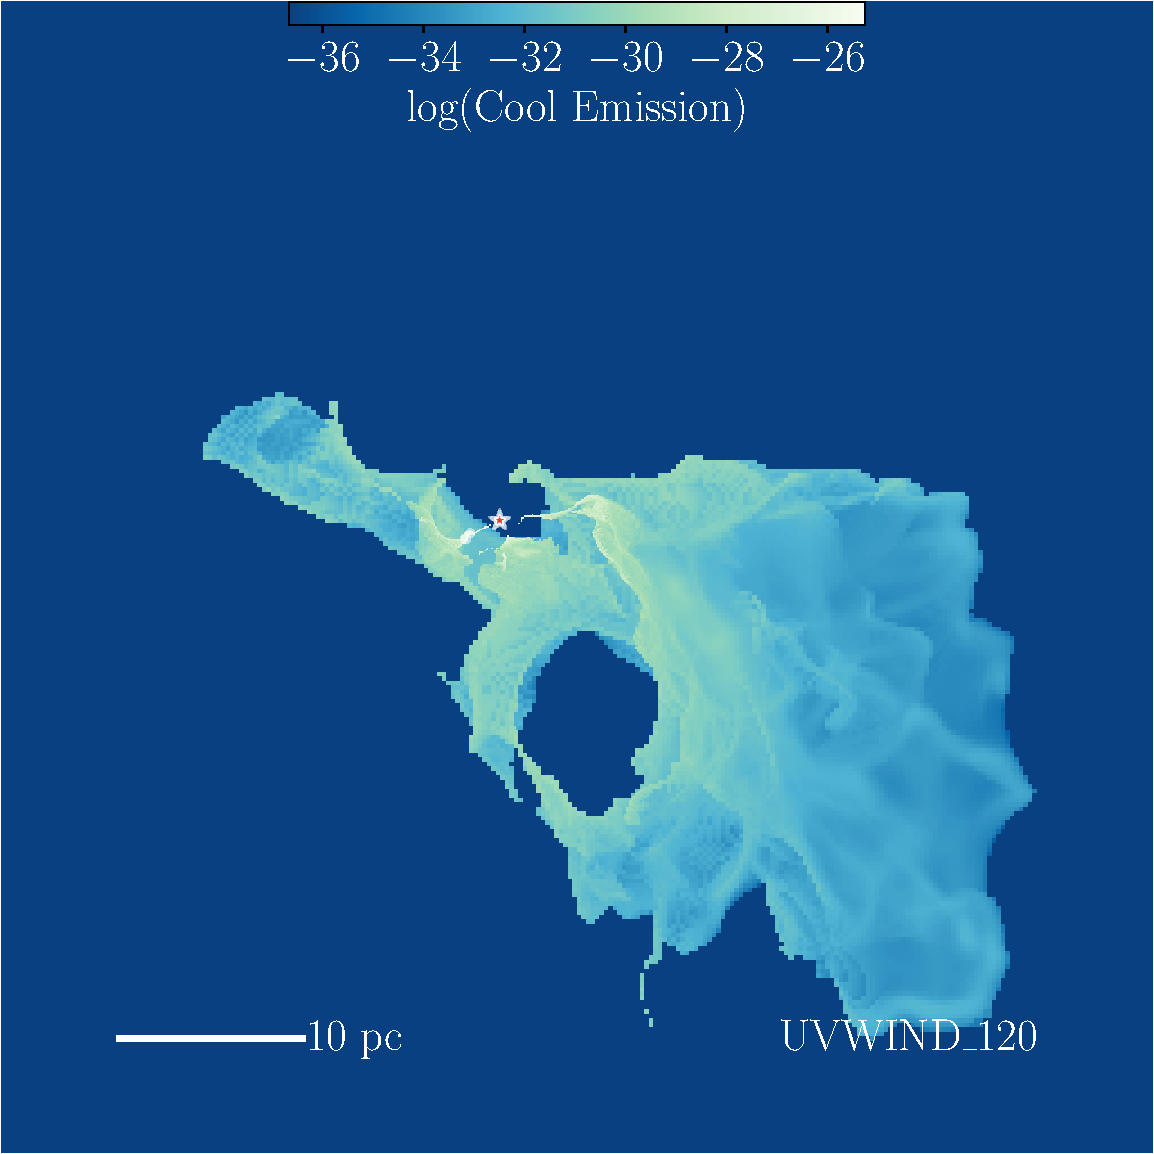
\includegraphics[width=0.66\columnwidth]{plots/fig10a.pdf} 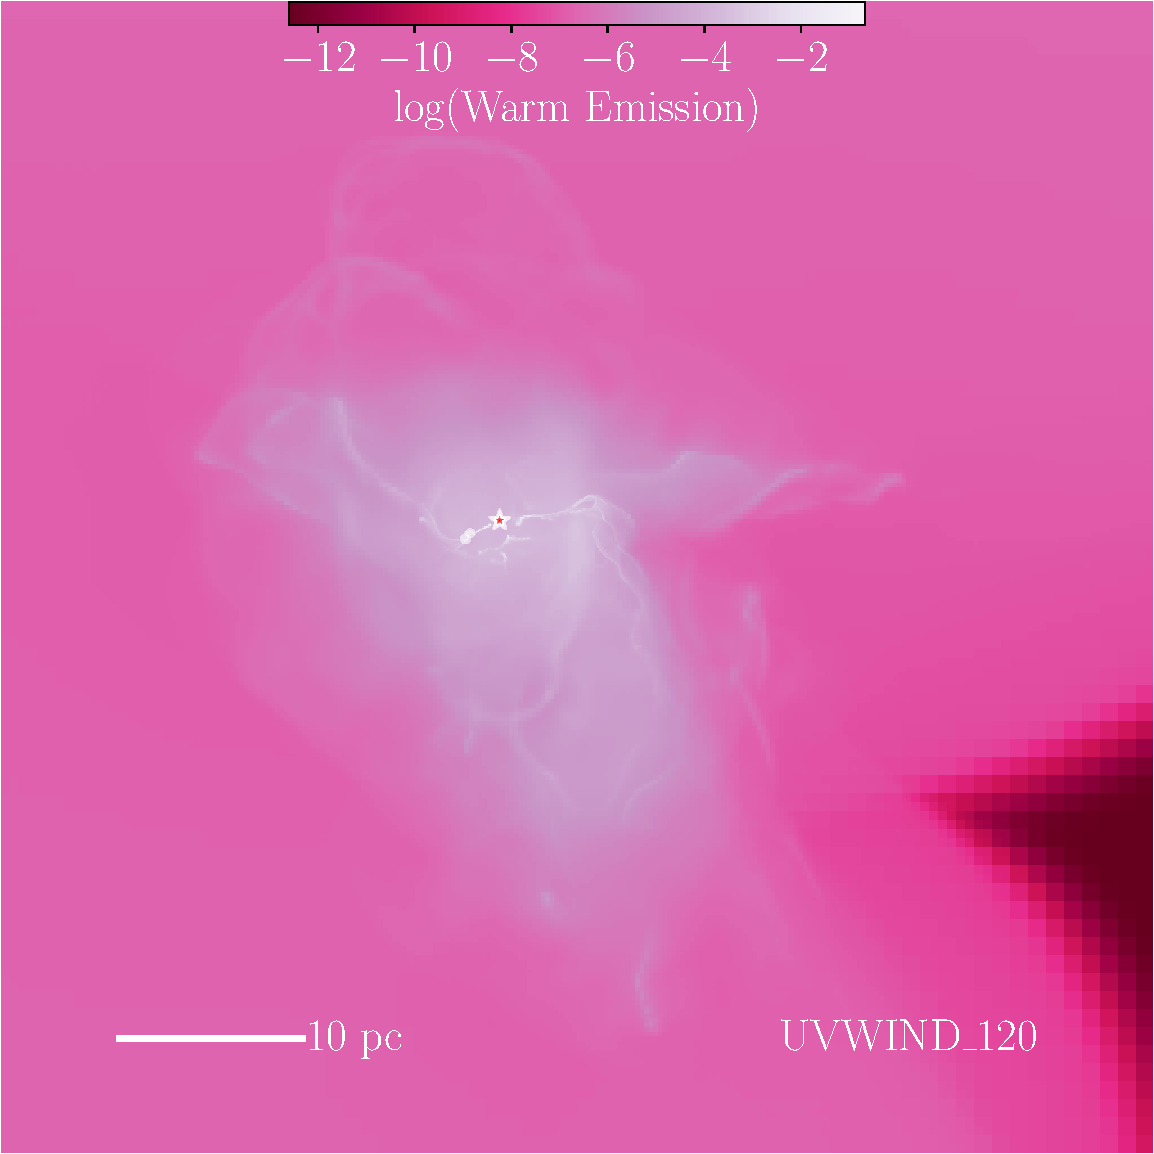
\includegraphics[width=0.66\columnwidth]{plots/fig10b.pdf}
	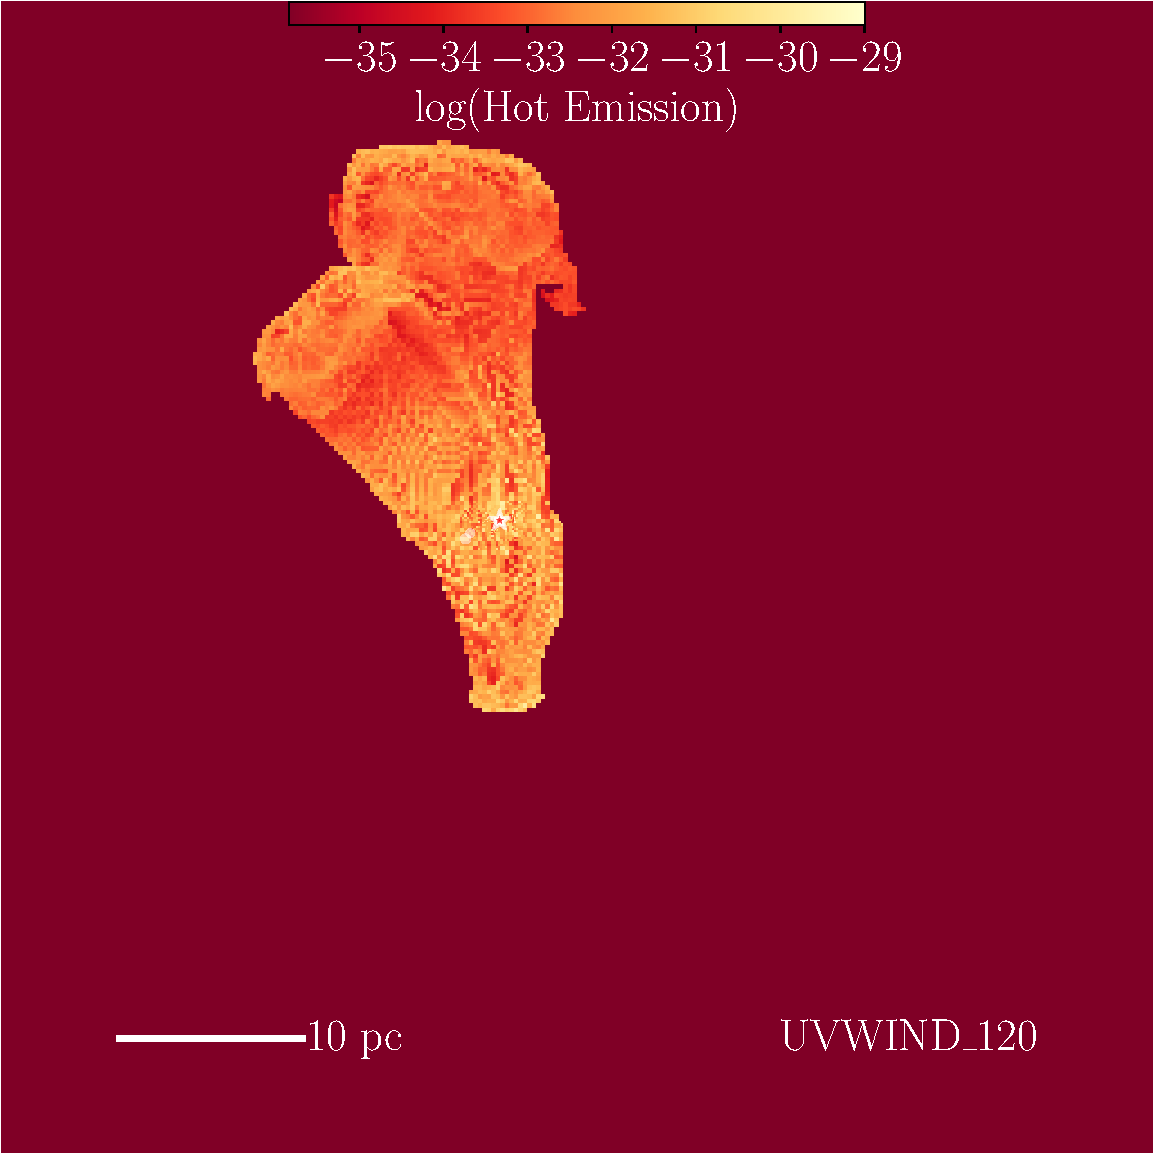
\includegraphics[width=0.66\columnwidth]{plots/fig10c.pdf}}
	\caption{Maps of radiative cooling of gas at different temperatures in the UVWIND\_120 simulation at 0.2 Myr after the 120 \Msolar star is formed. The left panel shows radiative cooling losses along the line of sight for gas below 1000 K. The middle panel shows recombination losses from photoionised gas ($n_e n_H$ projected along the line of sight). The right panel shows radiative cooling losses along the line of sight for gas above $10^6$ K. Each measure is not normalised and should be considered in relative terms. Full synthetic observations are beyond the scope of this paper.}
	\label{fig:emission_bands}
\end{figure*}


%\begin{figure*}
%	\centerline{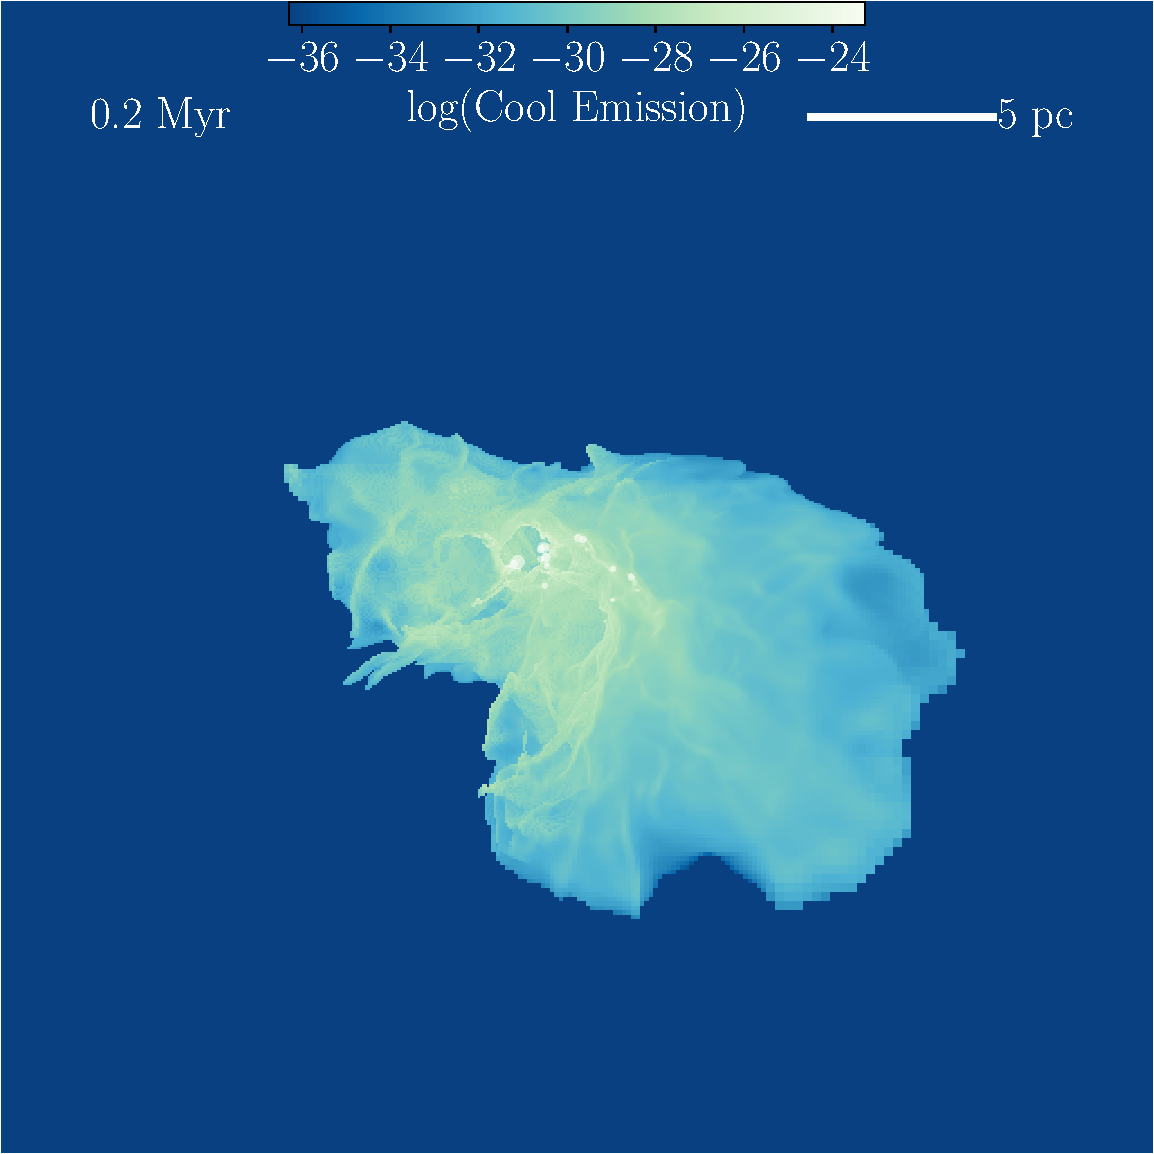
\includegraphics[width=0.66\columnwidth]{../plots/vis/multiray/multirayTime_coolemission_windset_120Msun_dense0p2Myr_zoom1p0__ywindonly.pdf} 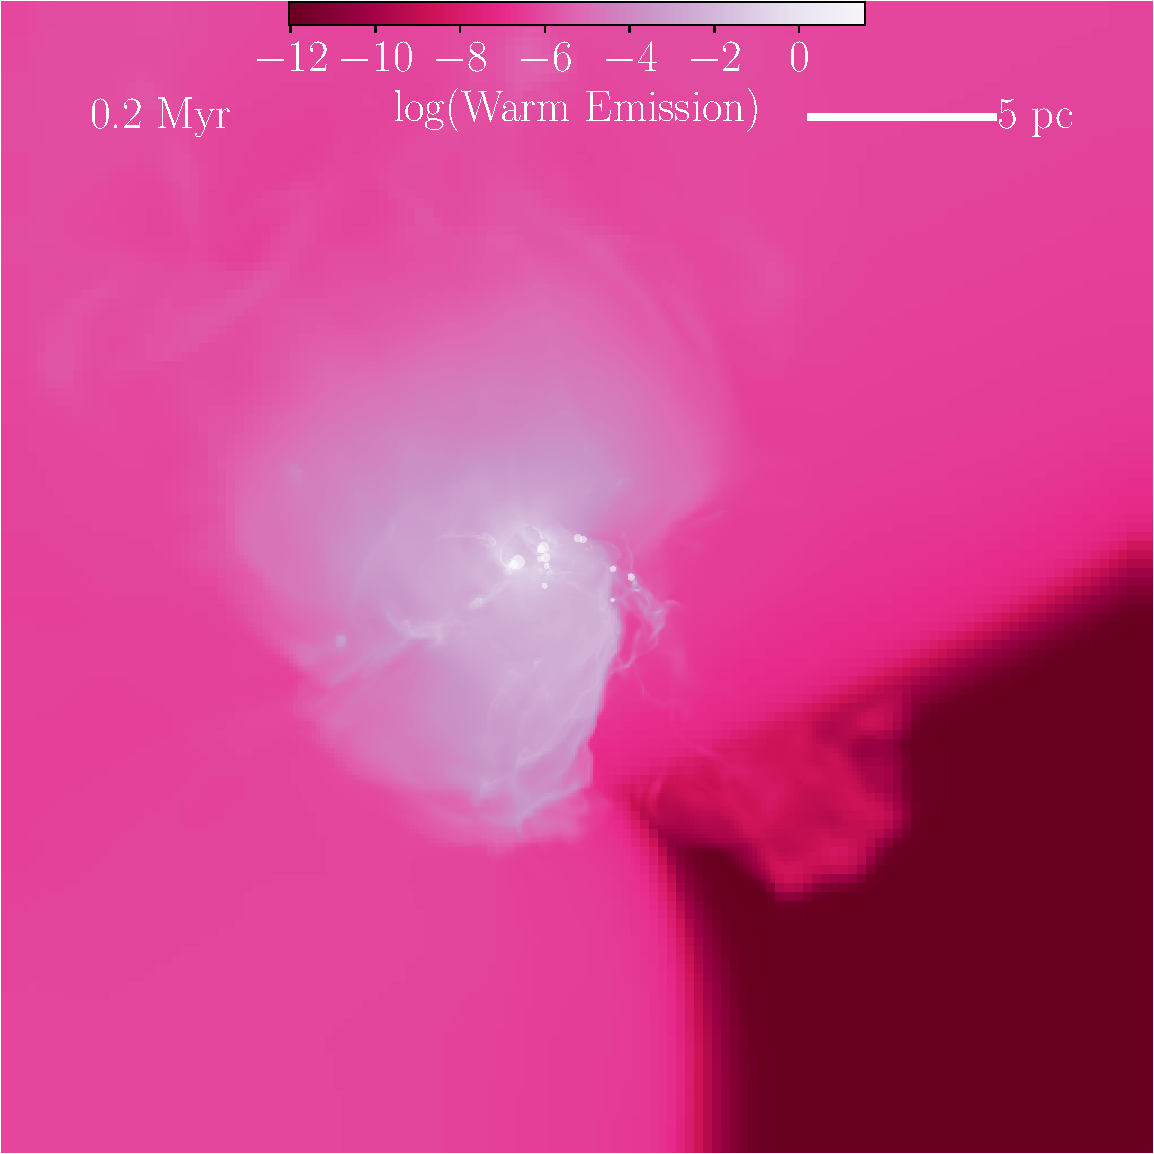
\includegraphics[width=0.66\columnwidth]{../plots/vis/multiray/multirayTime_ionemission_windset_120Msun_dense0p2Myr_zoom1p0__ywindonly.pdf}
%		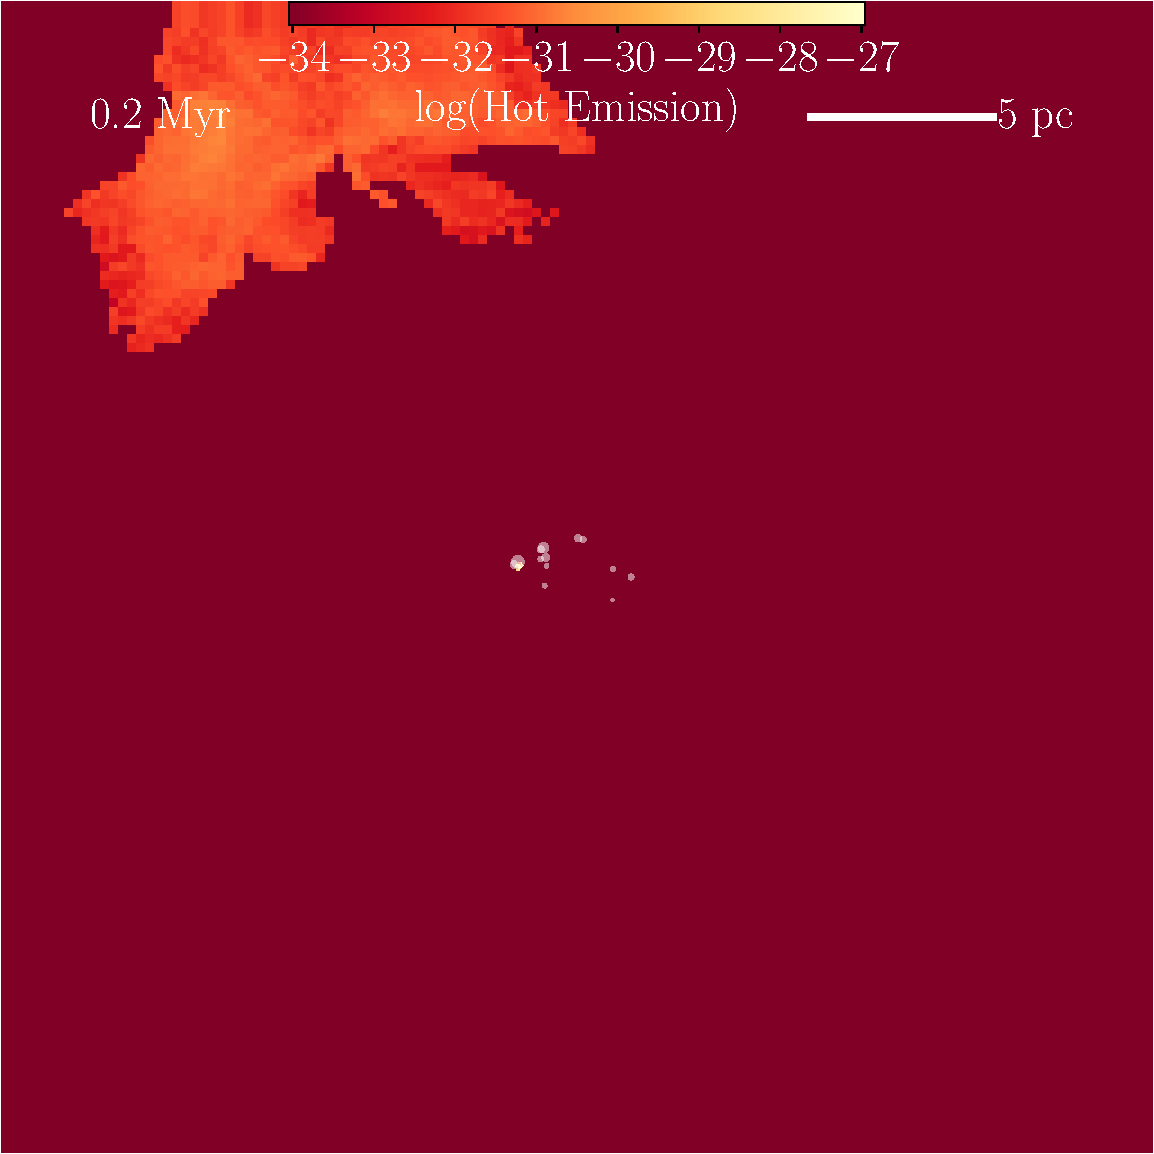
\includegraphics[width=0.66\columnwidth]{../plots/vis/multiray/multirayTime_xrayemission2_windset_120Msun_dense0p2Myr_zoom1p0__ywindonly.pdf}}
%	\caption{EMISSION PROPERTIES DENSE TEST}
%	\label{fig:emission_bands_dense}
%\end{figure*}

\begin{figure*}
	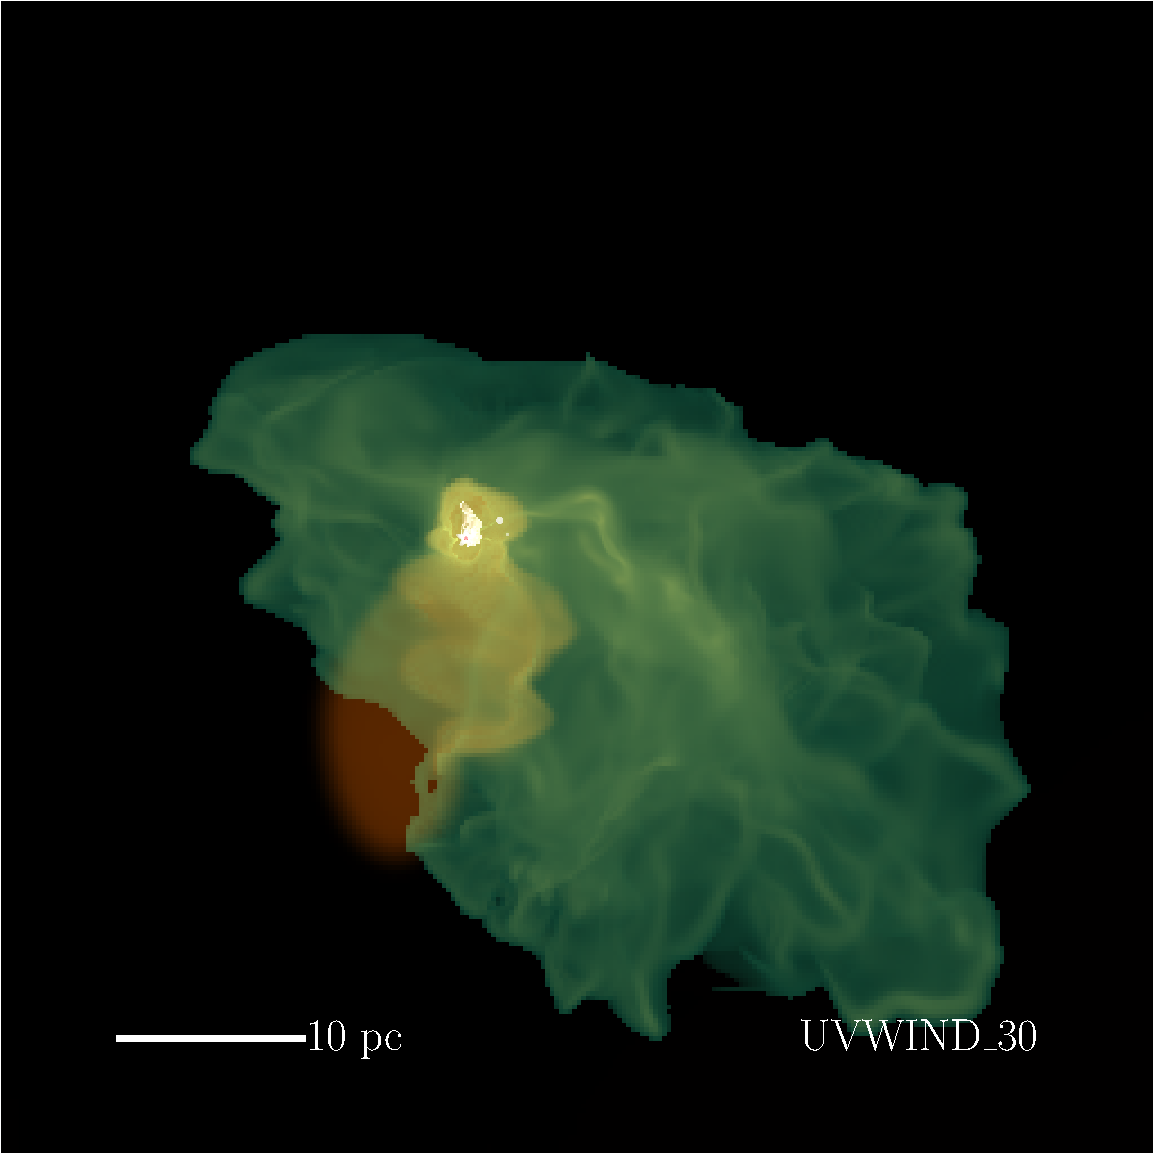
\includegraphics[width=0.99\columnwidth]{plots/fig11a.pdf} 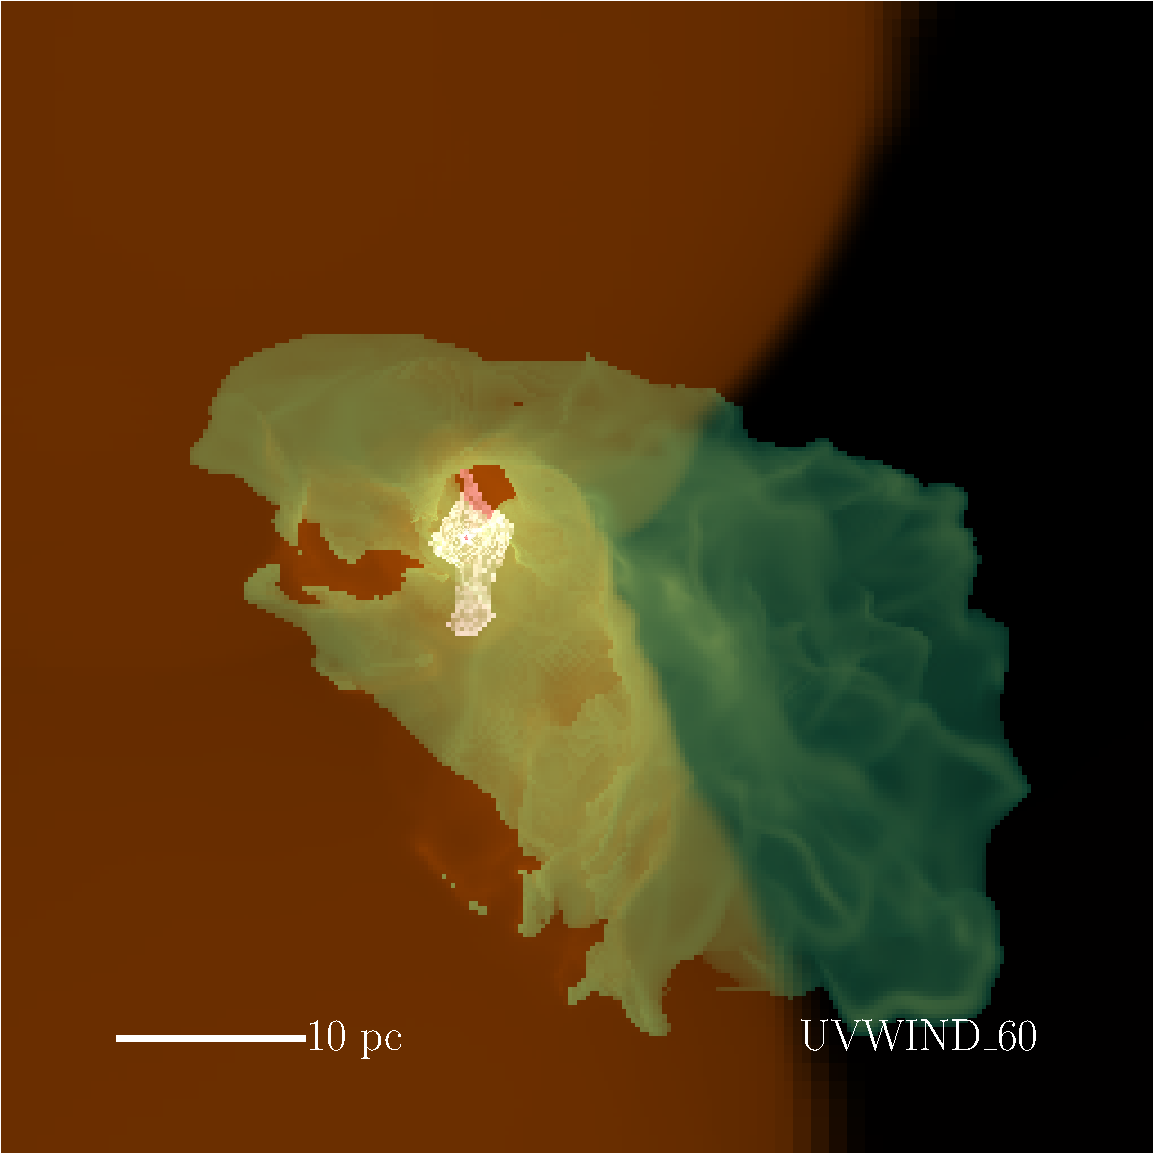
\includegraphics[width=0.99\columnwidth]{plots/fig11b.pdf}
	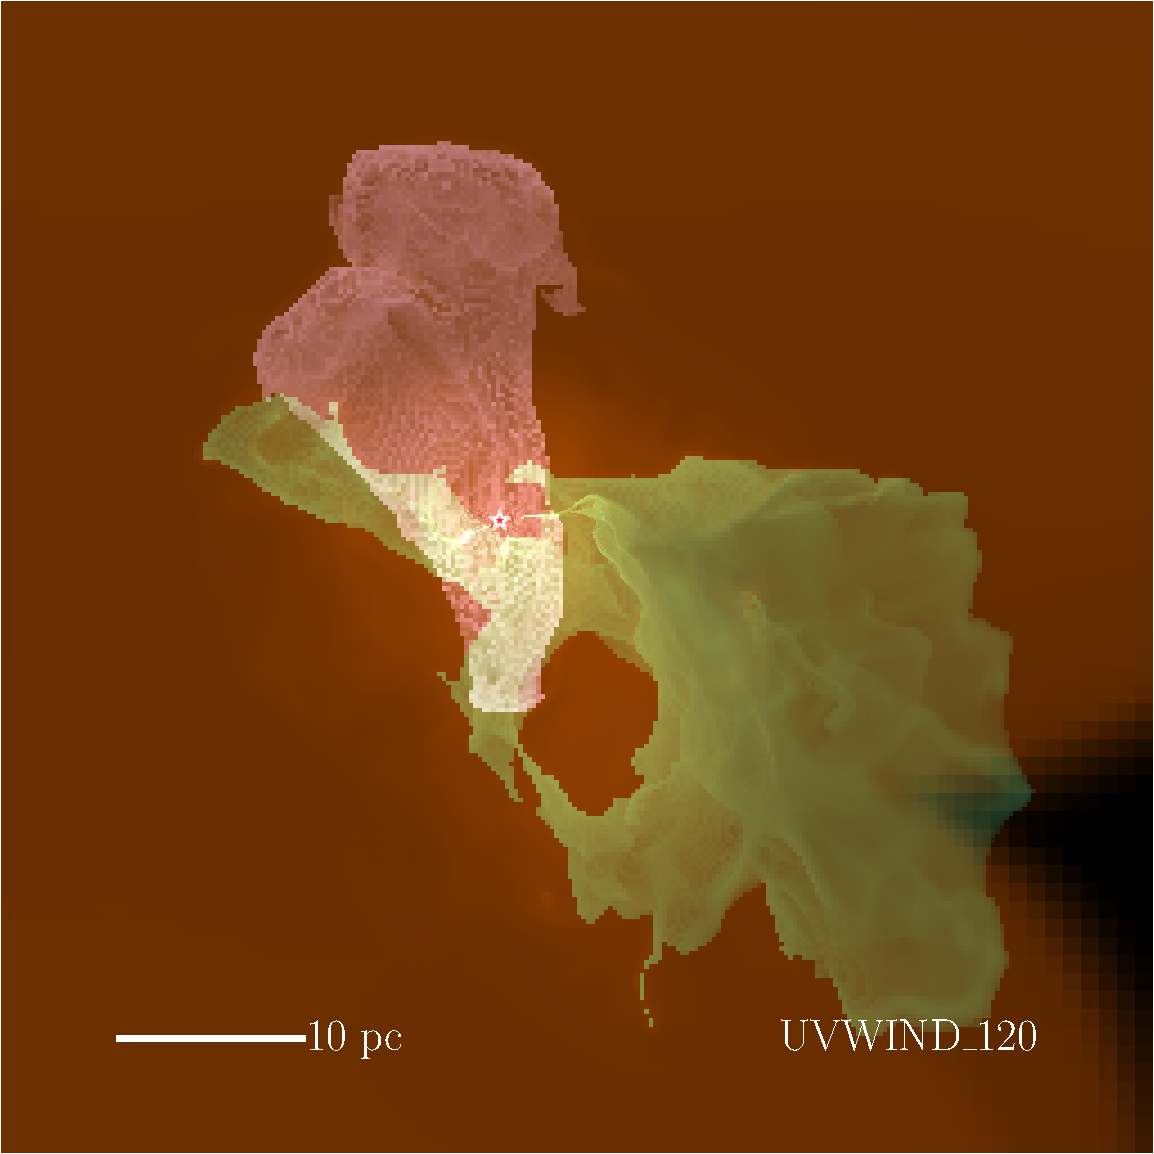
\includegraphics[width=0.99\columnwidth]{plots/fig11c.pdf} 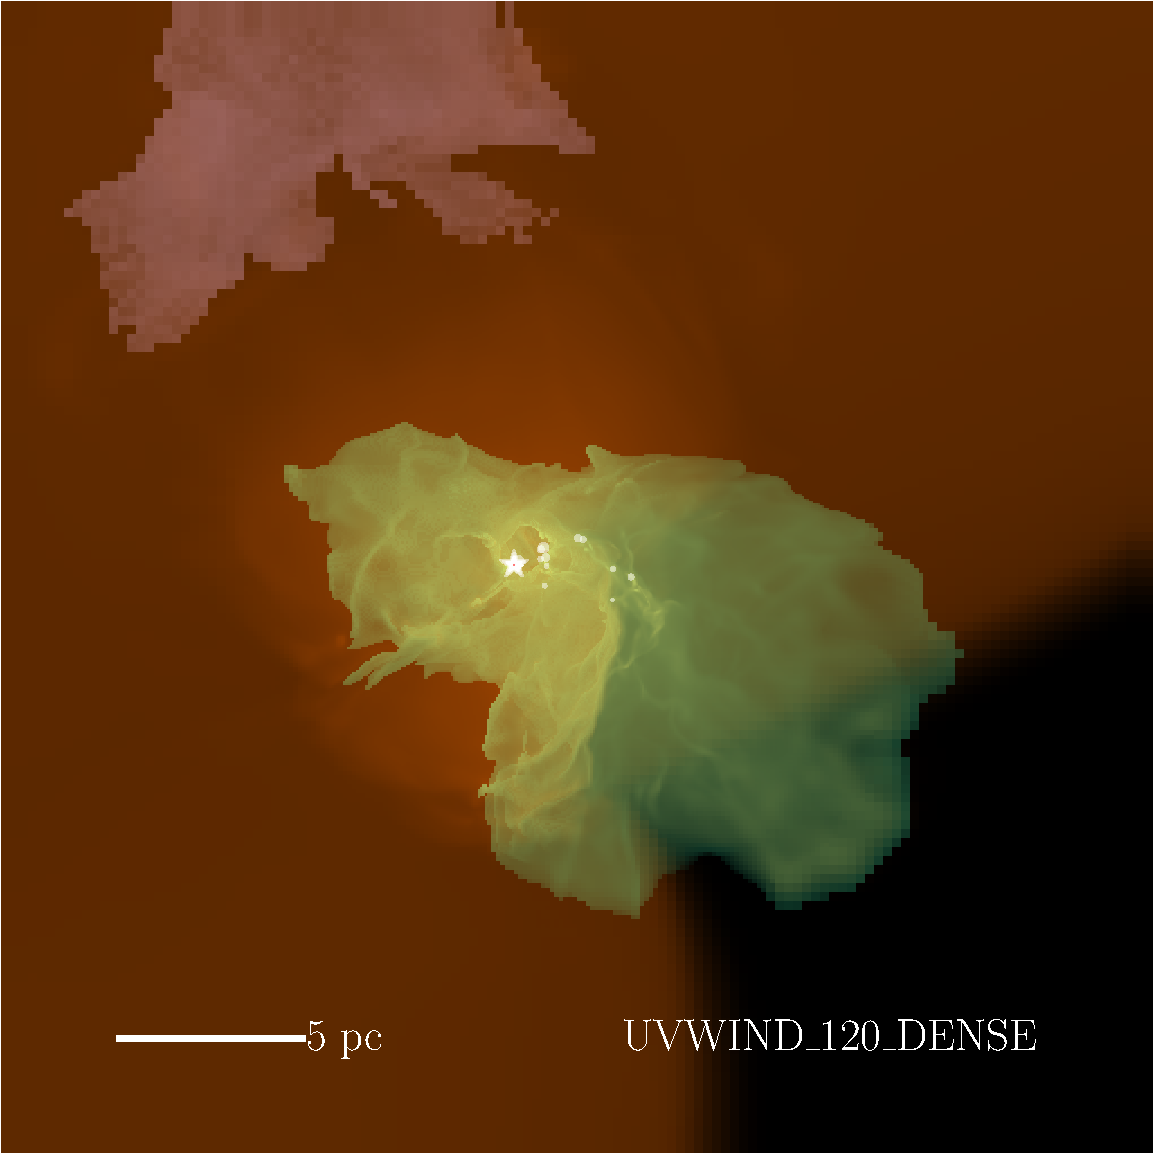
\includegraphics[width=0.99\columnwidth]{plots/fig11d.pdf}
	\caption{Maps of various radiative properties of the gas projected in the y axis in each simulation including stellar winds at 0.2 Myr after the star is formed, as shown individually in Figure \ref{fig:emission_bands}. Green shows the projected cooling rate of cool gas (below 1000 K). Orange shows the recombination rate in ionised gas. Purple shows the projected cooling rate of hot gas (above $10^6$ K). From top left to bottom right we plot results for the 30 \Msolar star, the 60 \Msolar star, the 120 \Msolar star, and the 120 \Msolar star in the \textsc{dense} cloud. Each value is normalised to arbitrary units for the purposes of visual comparison.}
	\label{fig:observability_yproj}
\end{figure*}

One question is whether extended wind bubbles are observable even when they are not the principal drivers of the \HII region. In Figure \ref{fig:emission_bands} we plot the total radiative emission by gas at various temperatures. We leave extensive synthetic observations for future work due to the complexity of the problem, and focus on the total radiative emission from cool, warm photoionised and hot structures. The left plot shows the cooling rate of gas below 1000 K. The middle plot shows a recombination emission measure, i.e. $n_e n_H$ where $n_e$ is the density of free electrions and $n_H$ is the hydrogen density. The right plot shows the cooling rate of gas above $10^6$ K.

Photoionised gas exists in all projected pixels in Figure \ref{fig:emission_bands}. Assuming that emission is calculated from a background baseline, the only detectable emission is from the ionised cloud before it has fully dispersed.

Cool gas remains to the right of the image, while hot gas is visible expanding upwards in the "ice cream" mode of wind feedback. Despite contributing at best 10\% of any given dynamical property to the system, extended wind emission is visible.

In Figure \ref{fig:observability_yproj} we overplot these bands for each simulation containing both photoionisation and winds. In Appendix \ref{appendix:emission_additional_projections} we include 2 further projections to illustrate the complex geometry of the wind bubbles in all simulations.

When the wind luminosity is strong enough, winds can easily escape the cloud, while not having a significant impact on properties such as \SFE or outflow momentum. This is because they have a significantly higher sound speed than the photoionised gas, and so rapidly follow pressure gradients to fill underpressurised volumes.

As stated in Section \ref{results:energeticswindbubble}, radiative losses from hot gas are only a small fraction of the total radiative losses of energy injected by the wind. Tracking the total radiative losses from winds is hard since they are masked by losses from the photoionised gas.

\subsection{Additional Factors}
\label{effective:intheend}

The conclusion of the paper thus far is that our simulations demonstrate that winds are not effective at driving outflows on molecular cloud scales. The broad findings of this work, including the energetics, are consistent with previous theoretical work. However, there are a number of possible differences between our simulations (and other relevant simulation work) and observed systems that would boost the dynamical efficiency of winds. 

There are additional factors that could increase the relative influence of winds versus photoionisation feedback not captured in these simulations. Firstly, radiation pressure (not included in this work) could drive the photoionised region into a denser shell as in \cite{Draine2011}. Authors such as \cite{Pellegrini2007} and \cite{Yeh2012} argue that winds further compress the photoionised, even if they are not the principal drivers of observed \HII regions. Denser photoionised regions have a higher recombination rate, increasing their cooling rate and reducing the efficiency of photoionisation.

Secondly, if the thickness of the mixing layer around the wind bubble is better resolved, there is the possibility that the hot bubble and denser photoionised gas are more separate, and hence the cooling rate from mixing is lower (see Section \ref{introduction}).

Thirdly, the presence of multiple massive stars in the same region can boost the effect of winds. In \cite{Geen2019} we predict that as the number of stars in one wind bubble increases, so does the relative efficiency of the winds. However, as stated in Section \ref{results:energeticswindbubble}, the cluster would have to be very large to make a significant impact.

Fourthly, our simulations have a relatively underdense external medium with no accretion. It is possible that \HII regions embedded in larger structures with inflows constraining their expansion would have different properties. For example, \cite{Pabst2019} find no evidence of wind breakouts in the Orion Veil nebula. More careful work comparing observed regions to simulations is needed to address this issue. In particular, full synthetic observations with accurate ray tracing are needed to account for the census of photons in different observable bands that are visible in observational studies.

Fifthly, this work focusses on the expansion of wind bubbles around young ($<$1 Myr old) stars. As \cite{Rahner2017} argues for older, more massive clusters, winds are boosted at late times relative to ionising radiation emission. However, this depends on the stellar evolution model used. \cite{Sana2012} observed that the majority of massive stars are in interacting binaries, strongly affecting their evolution. One of the results of this is that the extended envelopes of these stars are removed by binary interactions, allowing for higher ionising emission rates at late times. Accurate stellar evolution models are thus a crucial component in studies of feedback in \HII regions.

\section{Conclusions}
\label{conclusions}

We simulate a set of molecular clouds containing a single massive star of either 30, 60 or 120 \Msolar formed self-consistently using sink particles. We track photoionisation and stellar winds produced by the star.

As in other simulation work, we find that winds contribute at most 10\% to the reduction in SFE and outflow momentum in the first Myr of the lifetime of the star. Similarly, we find that winds cool efficiently over a short timescale ($\sim 10^4$ yr) compared to the lifetime of the star.

We show that one possible factor that confuses the interpretation of observed systems is that winds produce ``chimney-and-plume'' structures that efficiently tunnel through photoionised clouds to produce large, hot volumes of gas away from the sites of star formation. These are much more directional than the ``champagne'' flows produced by photoionisation. We also find a case where plumes exist without chimneys for 100-200 kyr. 

We demonstrate that this gives the impression that winds can appear to be volume-filling while also not contributing significantly to the regulation of star formation or outflows from the cloud. However, more work is needed to compare directly to observed systems and determine the underlying physics.

\section*{Acknowledgements}

ACKNOWLEDGEMENTS
Jo Puls, Xander Tielens, Cornelia Pabst, Patrick Hennebelle, Eric Pellegrini, Daniel Rahner, Ralf Klessen, Lex Kaper

The authors gratefully acknowledge the data storage service SDS@hd supported by the Ministry of Science, Research and the Arts Baden-W\"urttemberg (MWK) and the German Research Foundation (DFG) through grant INST 35/1314-1 FUGG.
CARTESIUS

%%%%%%%%%%%%%%%%%%%%%%%%%%%%%%%%%%%%%%%%%%%%%%%%%%

%%%%%%%%%%%%%%%%%%%% REFERENCES %%%%%%%%%%%%%%%%%%

% The best way to enter references is to use BibTeX:

\bibliographystyle{mnras}
\bibliography{samgeen} % if your bibtex file is called example.bib

%%%%%%%%%%%%%%%%%%%%%%%%%%%%%%%%%%%%%%%%%%%%%%%%%%

%%%%%%%%%%%%%%%%% APPENDICES %%%%%%%%%%%%%%%%%%%%%

\appendix
%
%\section{Appendix Blah}
%
%APPENDIX
\section{Emission - Additional Projections}
\label{appendix:emission_additional_projections}

In order to better illustrate the complex geometry of the different structures in the simulated \HII regions, we present additional projections of the structures shown in Figure \ref{fig:observability_yproj}. These are shown in Figures \ref{fig:observability_xproj} and \ref{fig:observability_zproj}


\begin{figure*}
	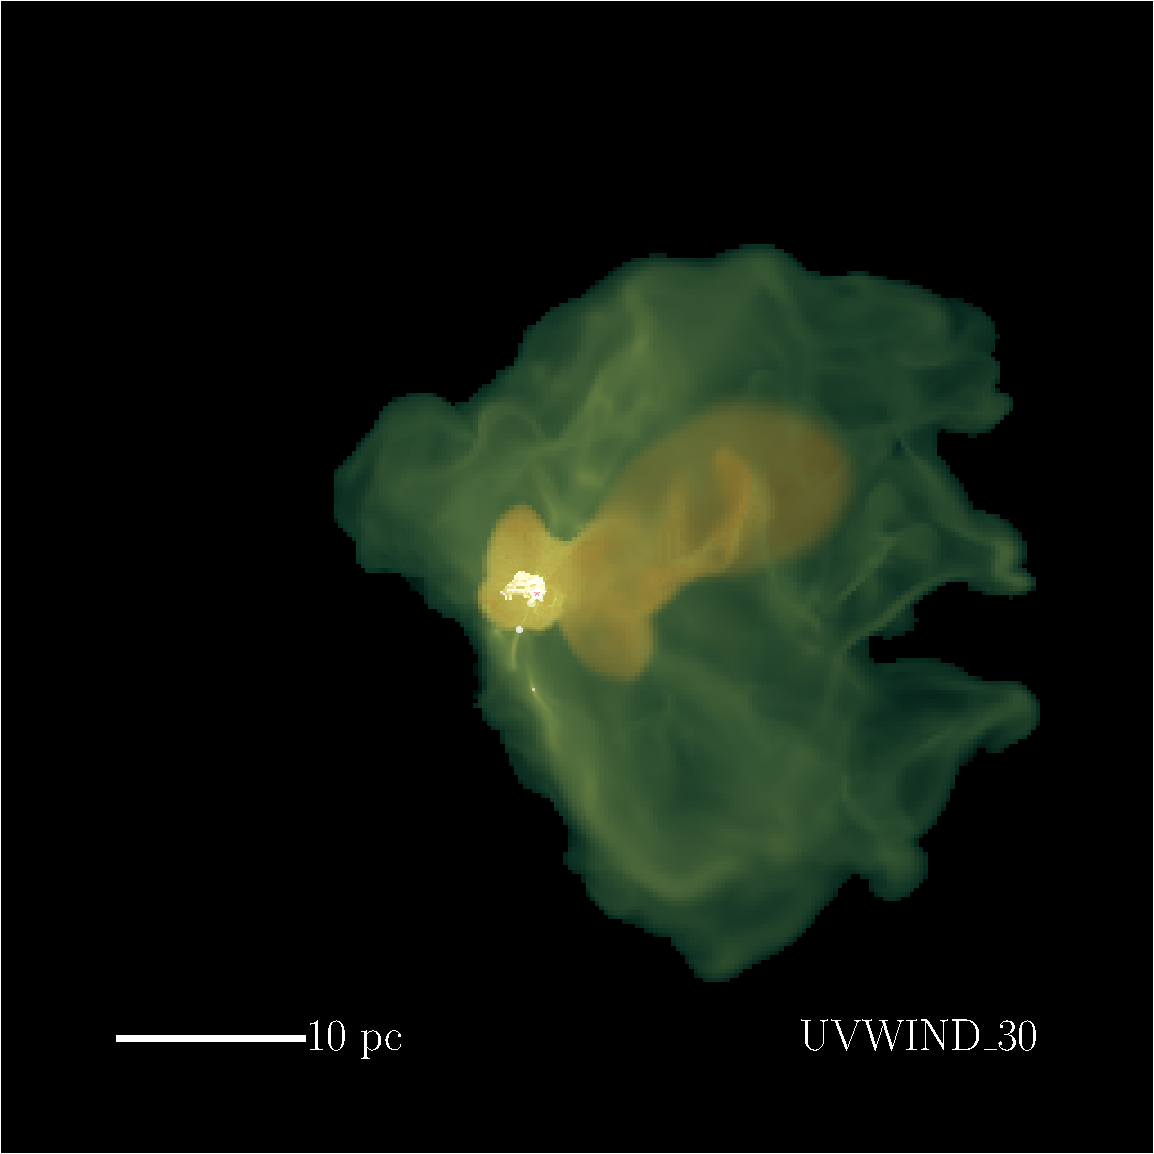
\includegraphics[width=1\columnwidth]{plots/fig12a.pdf} 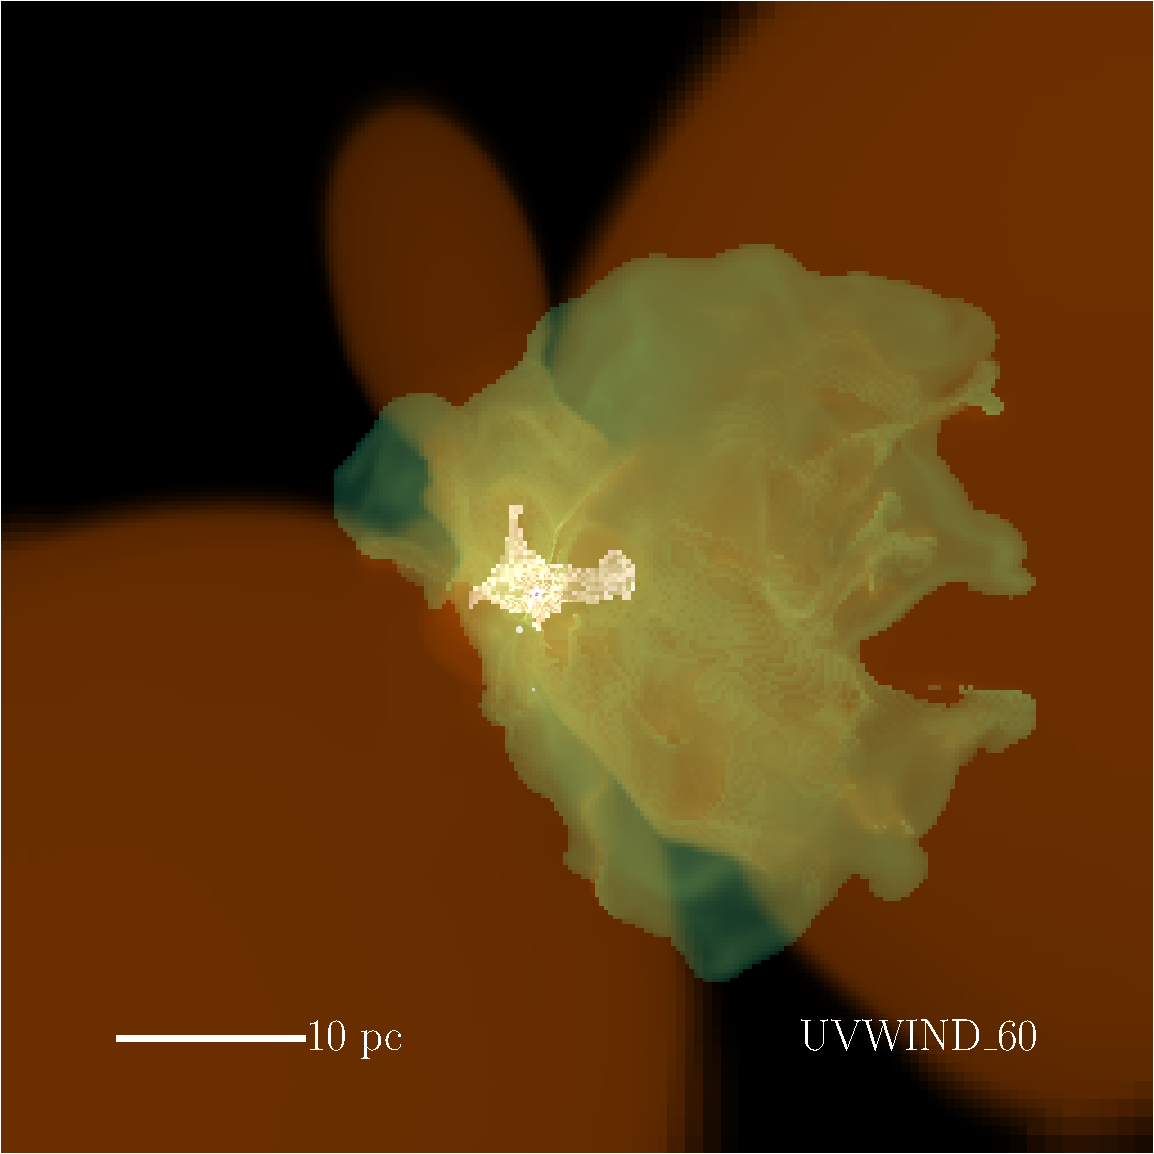
\includegraphics[width=1\columnwidth]{plots/fig12b.pdf}
	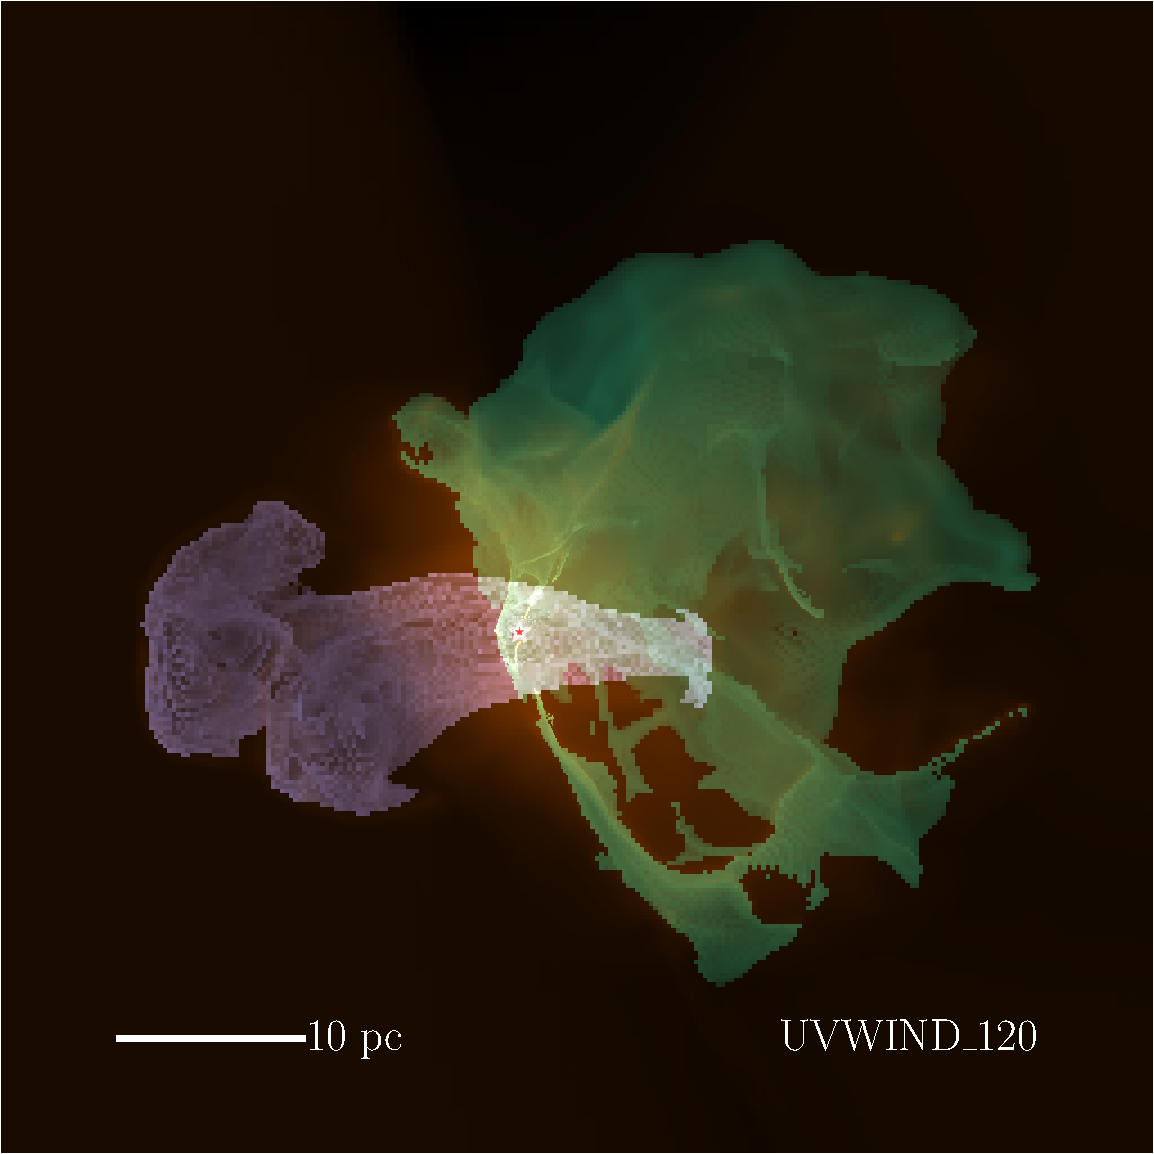
\includegraphics[width=1\columnwidth]{plots/fig12c.pdf} 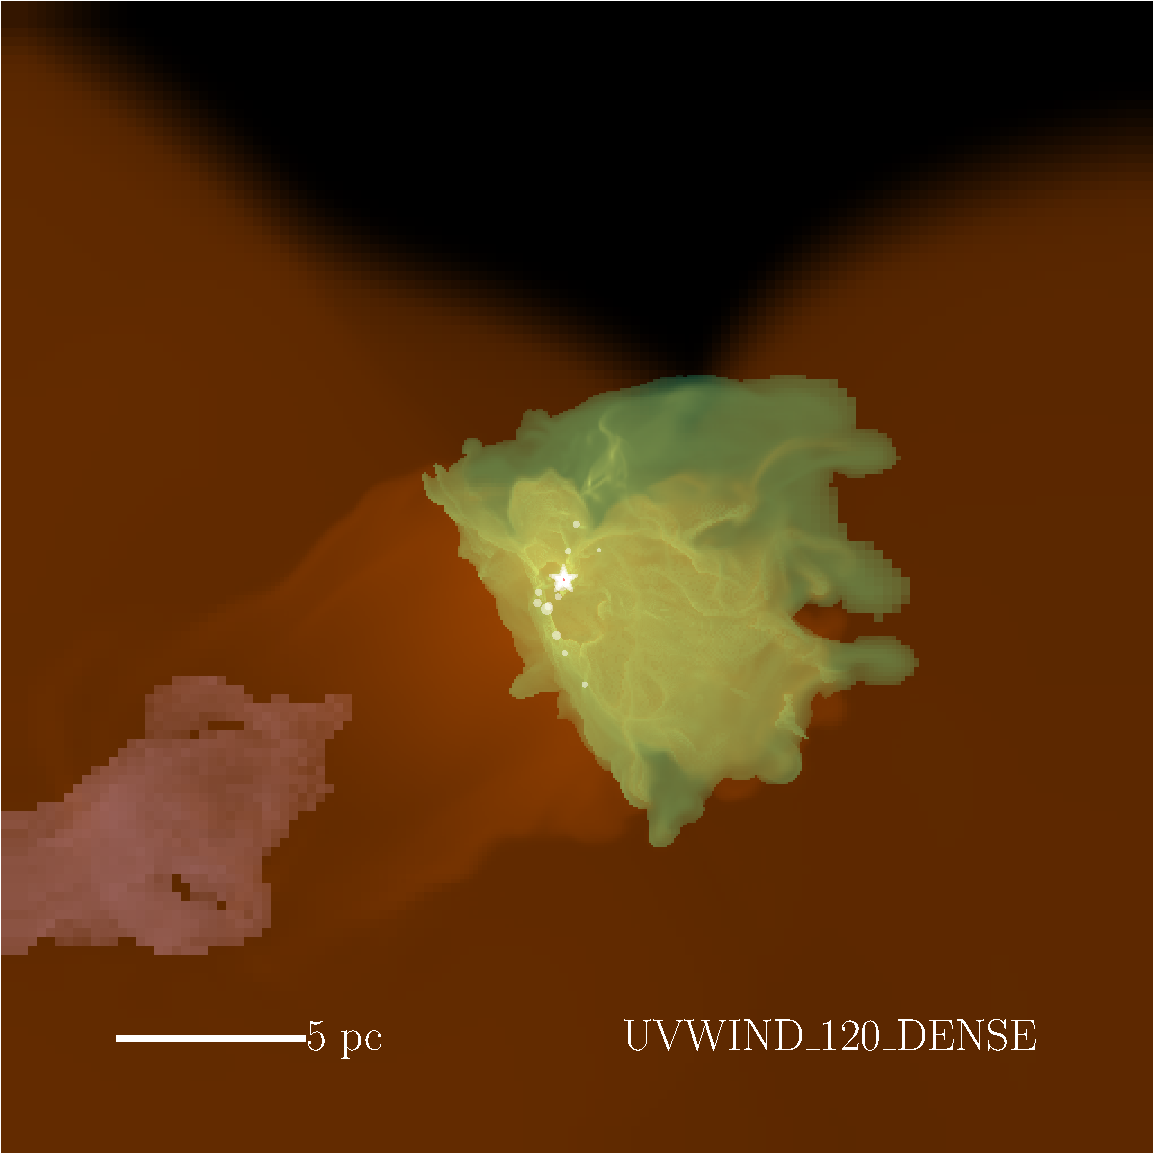
\includegraphics[width=1\columnwidth]{plots/fig12d.pdf}
	\caption{As in Figure \ref{fig:observability_yproj} but in the x axis.}
	\label{fig:observability_xproj}
\end{figure*}

\begin{figure*}
	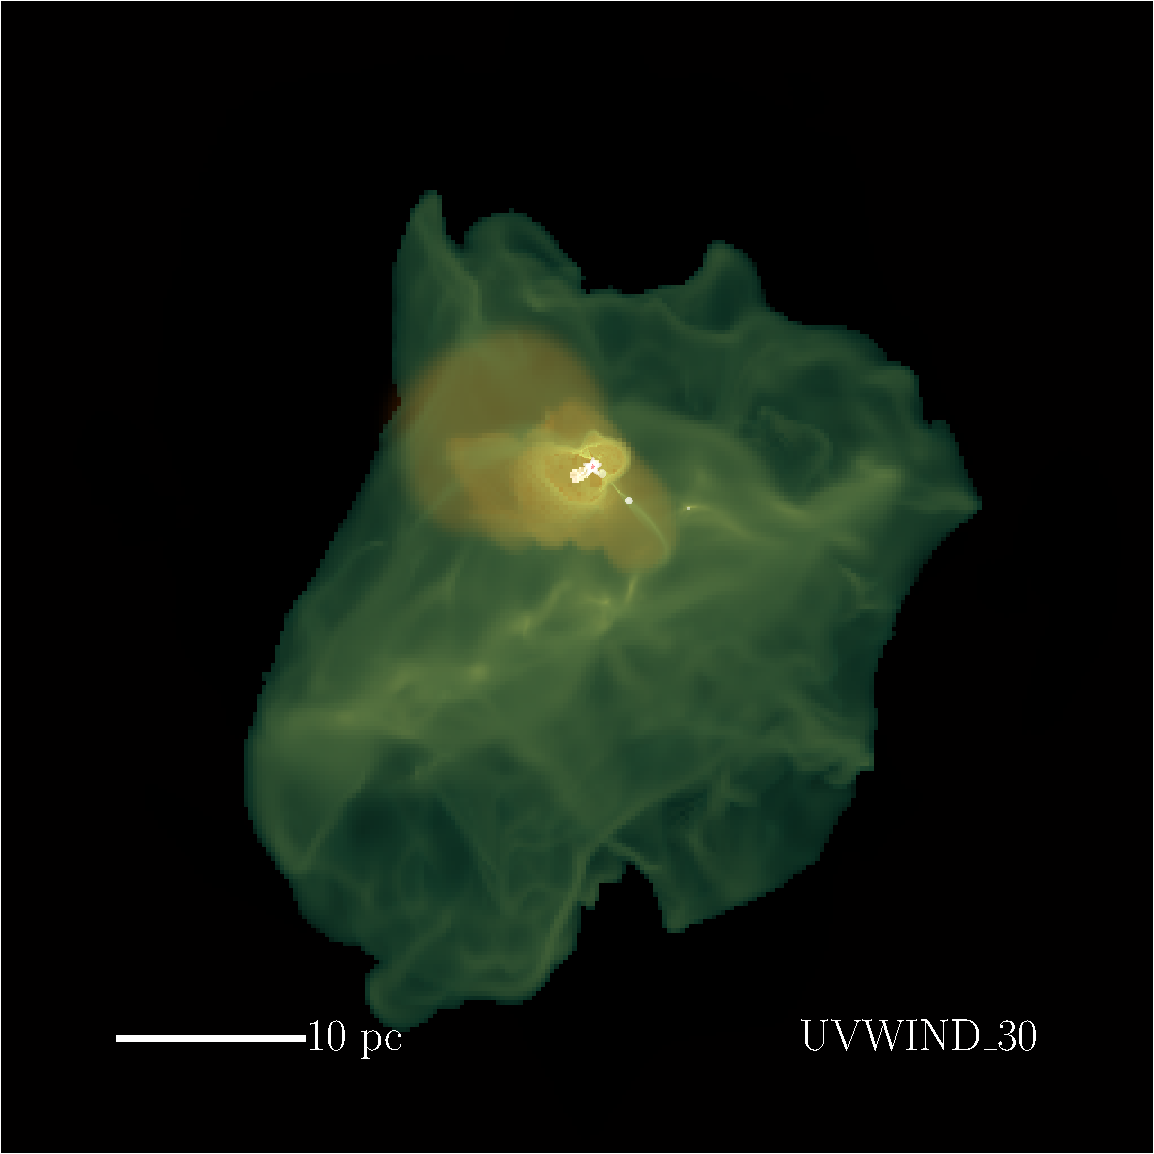
\includegraphics[width=1\columnwidth]{plots/fig13a.pdf} 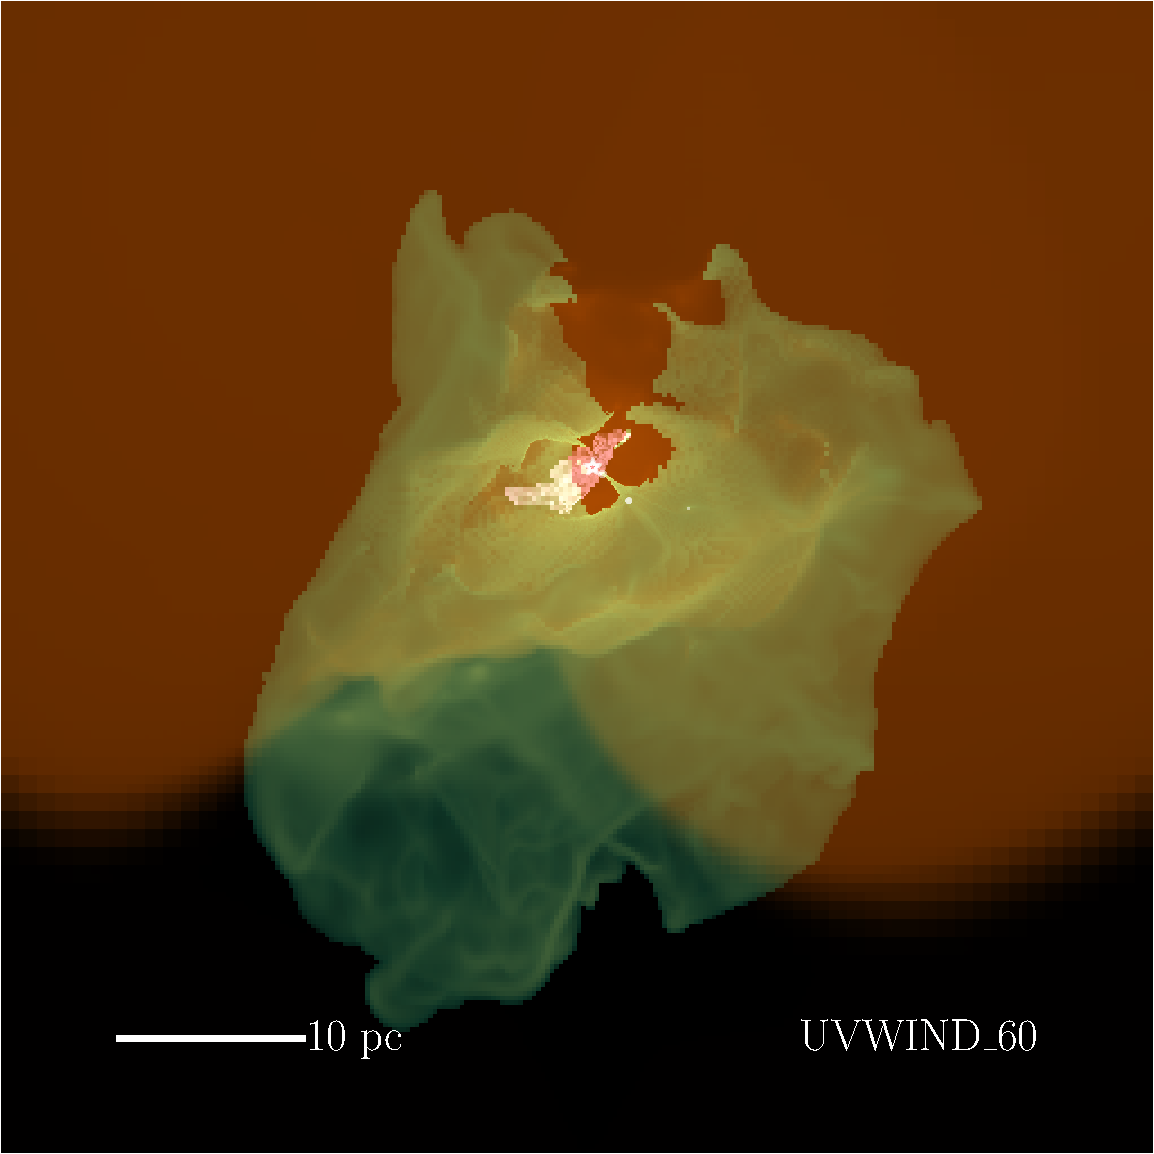
\includegraphics[width=1\columnwidth]{plots/fig13b.pdf}
	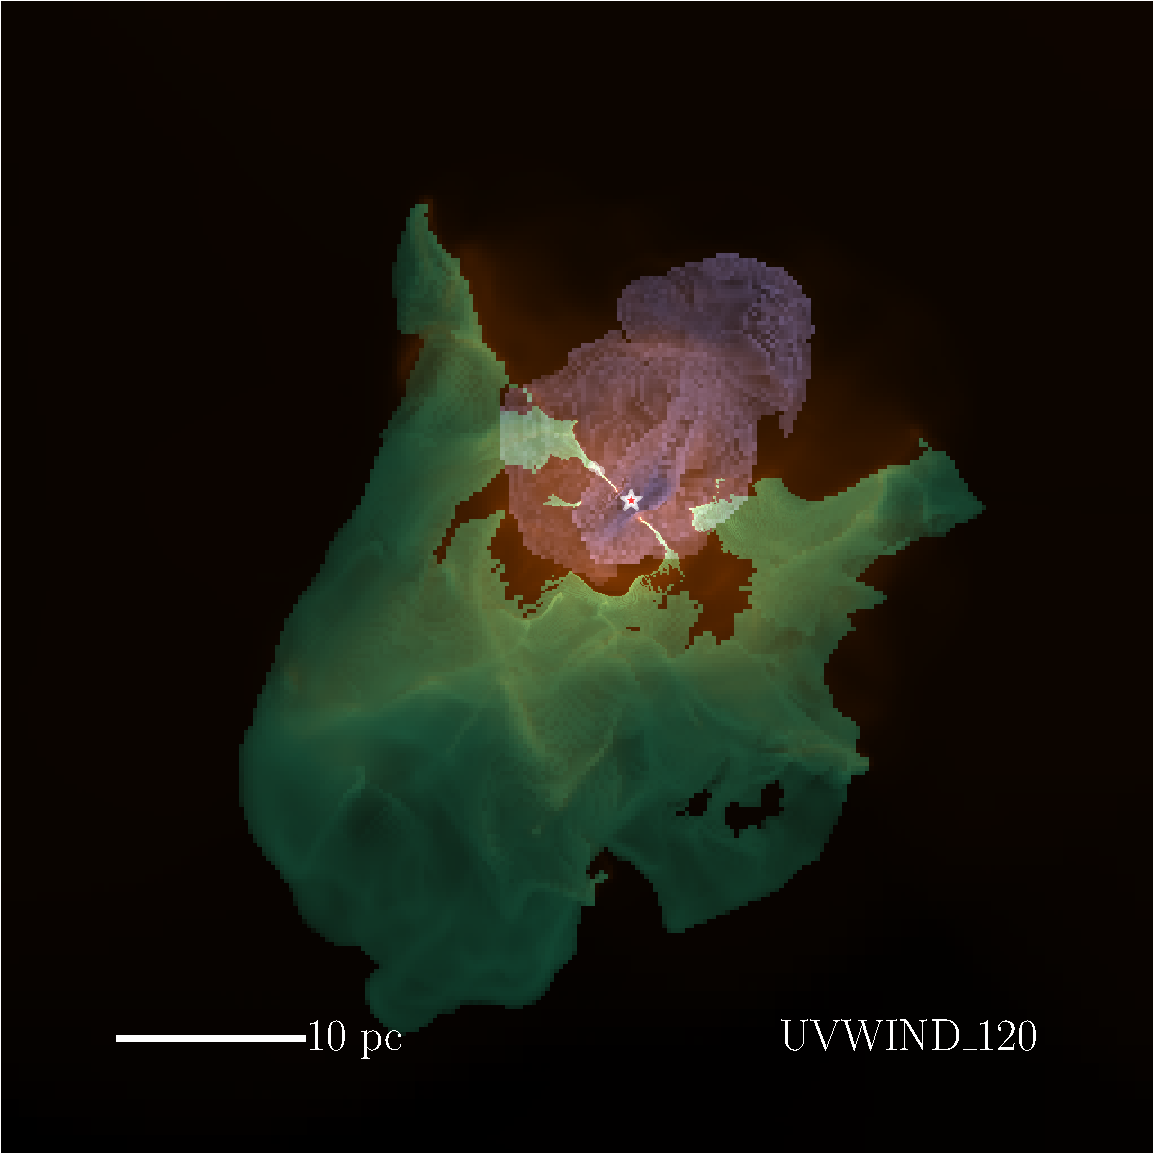
\includegraphics[width=1\columnwidth]{plots/fig13c.pdf} 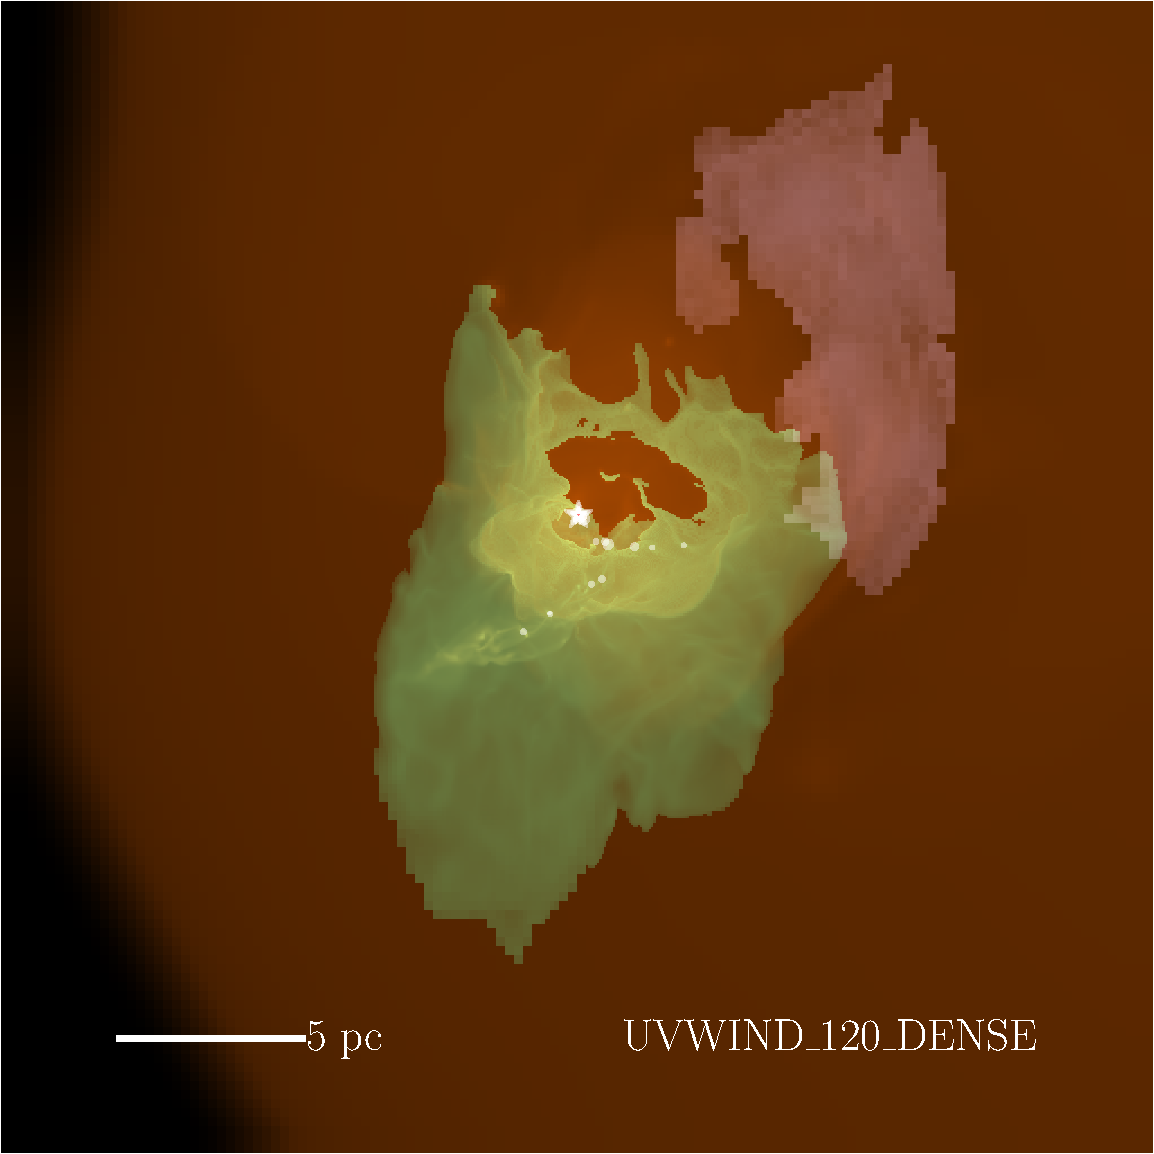
\includegraphics[width=1\columnwidth]{plots/fig13d.pdf}
	\caption{As in Figure \ref{fig:observability_yproj} but in the z axis.}
	\label{fig:observability_zproj}
\end{figure*}

%%%%%%%%%%%%%%%%%%%%%%%%%%%%%%%%%%%%%%%%%%%%%%%%%%


% Don't change these lines
\bsp	% typesetting comment
\label{lastpage}
\end{document}

% End of mnras_template.tex